\documentclass[a4paper,11pt]{article}

%\usepackage[pdftex]{graphicx}
\usepackage{amsmath}
\usepackage[skip=0.5\baselineskip]{caption}
%\usepackage[latin1]{inputenc}
%\usepackage{hyperref}
%\usepackage[T1]{fontenc}
%\usepackage[utf8]{inputenc}
%%GD Quand je mets usepackage[utf8]{inputenc} je n'arrive plus à compiler la biblio
%J'ai essayé de débuger : je n'y suis pas arrivé
\usepackage{rotating}
\usepackage{setspace}
\usepackage{lscape}
\usepackage[round]{natbib}
\usepackage{multirow}
\usepackage{rotating}
\usepackage{vmargin}
\usepackage{epstopdf}
\usepackage{hyperref}
\usepackage{float}
\usepackage{caption}
\usepackage[tableposition=top]{caption}
\usepackage{amsfonts}
\usepackage{bbold}
\usepackage{natbib}
\usepackage{babel,varioref}
\usepackage{bbm}
\usepackage[flushleft]{threeparttable}
%\usepackage{bbold}
%\usepackage[T1]{fontenc}
% JH : impossible de compiler avec le package bbold, remplacé par amsfonts
% LP : impossible de compiler avec le package bbold, remplacé par bbm
\usepackage{upgreek}
\usepackage{comment}
\includecomment{commentGD}
\usepackage[draft]{todonotes}
%\usepackage[disable]{todonotes}
%%GDPour cacher les notes, \usepackage[disable]{todonotes}

\usepackage{setspace}

%\usepackage[nolists, figuresfirst]{endfloat}
%\usepackage{sidefloat}

\setlength{\abovecaptionskip}{-8pt}

%\usepackage[usenames]{color}
%\definecolor{grey}{rgb}{0.35,0.35,0.35}
%\definecolor{webdarkblue}{rgb}{0,0,0.4}
%\definecolor{orange}{rgb}{0.7,0.2,0.05}


%\usepackage[pdfcreator={PDFLaTeX}, pdfproducer={PDFLaTeX}, pdfstartview=FitH, pdfpagemode=UseOutlines, pagebackref=false, colorlinks={true},
%citecolor={webdarkblue}, linkcolor={webdarkblue},
%urlcolor={webdarkblue}]{hyperref}



%\addtolength{\oddsidemargin}{-0.4in}
%\addtolength{\evensidemargin}{-0.4in}
%\addtolength{\textwidth}{0.8in} \addtolength{\topmargin}{-0.85in}
%\addtolength{\textheight}{1.7in}
\renewcommand{\baselinestretch}{1.2}

\newcommand\cites[1]{\citeauthor{#1}'s\ (\citeyear{#1})}

\newcommand\citeh[1]{\citeauthor{#1}'\ (\citeyear{#1})}

\setmarginsrb{3cm}{2cm}{3cm}{2cm}{0,5cm}{0,5cm}{0,3cm}{0,5cm}



% commands

\newcommand{\bi}{\begin{itemize}}
\newcommand{\ei}{\end{itemize}}
\newcommand{\be}{\begin{enumerate}}
\newcommand{\ee}{\end{enumerate}}
\newcommand{\bd}{\begin{description}}
\newcommand{\ed}{\end{description}}
\newcommand{\beqa}{\begin{eqnarray}}
\newcommand{\eeqa}{\end{eqnarray}}
\newcommand{\beq}{\begin{equation}}
\newcommand{\eeq}{\end{equation}}
\newcommand{\bs}{\bigskip}
\newcommand{\A}{$^a$}
\newcommand{\B}{$^b$}
\newcommand{\C}{$^c$}

\renewcommand{\baselinestretch}{1.2}
%\doublespacing

%\linespread{1.6}

%\newcommand{\note}[1]{\footnote{\begin{doublespace}#1\end{doublespace}}}

%\citesep{knuth-681,knuth-702}{'s work

\begin{document}




\title{\textsc{International Transport costs:\\New Findings from modeling additive costs}\thanks{We thank the referees, as well as the editor, William Kerr, for insightful comments, which helped to significantly improve the paper. We are grateful to Holger G\"{o}rg, S\'{e}bastien Jean and Vincent Vicard for their critics and suggestions on earlier drafts. The paper has also greatly benefited from remarks from the participants at ETSG 17\textsuperscript{th} (Helsinki), DEGIT XXII (Paris), seminars at the universities of California-Irvine, Paris-Dauphine, Paris-I and Nancy and the Kiel Institute for the World Economy. Any remaining errors are ours. This paper was partly funded by a university grant from the University of Lille. It features an online appendix containing additional results, available on the authors' websites and on \url{https://github.com/gdaudin/trade_costs}.}}

\author{Guillaume \textsc{Daudin}\thanks{%
University Paris-Dauphine \& PSL University, IRD, LEDa, UMR 225, DIAL, 75016 Paris, France; email: \url{guillaume.daudin@dauphine.psl.eu}}  \qquad J\'{e}r\^{o}me \textsc{H\'{e}ricourt} \thanks{Univ. Lille, CNRS, IESEG School of Management, UMR 9221 - LEM - Lille Économie Management, F-59000 Lille, France, and CEPII, France; email: \url{jerome.hericourt@univ-lille.fr}}\qquad Lise \textsc{Patureau}\thanks{Corresponding author.
University Paris-Dauphine \& PSL University, LEDa, 75016 Paris, France;  email: \url{lise.patureau@dauphine.psl.eu} } }


\date{November 2021}
 \maketitle
\bigskip

\begin{abstract}
International transport costs do have an additive part. How large is it? Does it matter? This paper provides new answers to these questions. Using information contained in the US imports flows from 1974 to 2019, we develop an empirical model that disentangles the ad-valorem and the additive components of international transport costs. The per-unit component of transport costs represents a sizeable share of total transport costs, between 30\% and 45\% depending on the year and the transport mode considered. We then investigate the important consequences of additive costs, under two different perspectives. First, modelling varying additive costs modifies the decomposition of transport costs time trend between the reduction in ``pure'' transport costs and trade composition effects, the latter playing a minor role. Second, we revisit the welfare gains of the transport cost reduction in presence of additive costs. In this regard, we shed light on the welfare variations induced by the ``hyper-globalization'' period, as well as the key role of additive transport costs in determining those welfare variations. Neglecting the additive component substantially underestimates the welfare gains of the transport cost decrease.
\end{abstract}


\thispagestyle{empty} \pagestyle{plain} \setcounter{page}{1}

\bigskip


\noindent \emph{JEL classification}: F10, N70, R40 \\
\noindent \emph{Keywords}: Transport costs estimates, non-linear econometrics, period 1974-2019, additive costs, trade composition effects, gains from trade

{\normalsize \vspace{0cm} }

{\normalsize \titlepage }

{\normalsize \newpage }

%\begin{spacing}{1.5}

\section{Introduction \label{sec:Intro}}


Trade costs are central to international economic analysis. In particular, they are a major obstacle to international trade flows. Defined as the costs associated with the exchange of goods across national borders, trade costs are usually split between transaction costs, policy costs, time costs and transport costs. Many argue that the latter have substantially decreased thanks to technological advance in transportation, infrastructure development and new communication technologies.
However, several empirical studies suggest that transport costs remain large and deserve attention.\footnote{\cite{anderson_wincoop_jel} find that around 30\% of international trade costs are attributable to transport costs. Equivalently, international transportation costs represent a 21\% markup over production costs. Further, the sizable elasticity of trade with respect to freight costs obtained by \cite{Behar_Venables} (around -3) attests to the impact of transport costs on trade flows. \cite{Disdier_Head08}, among others, point out that distance as an incompressible cost is still a very important determinant of trade flows.} In addition, progress in transportation techniques (which reduces the constant-dollar cost of transport) should be compared with technical progress in production (which reduces the constant-dollar cost of production) to get a clear picture of the evolution
of the transport costs burden. The latter also depends on whether the transport costs are in proportion to the value of goods traded (hence do not distort relative prices) or are not related to the value of goods traded (hence do distort relative prices). Having a clear view of the international transport cost burden is a complex task, but of key importance. Indeed, the answers to several important (both academic and policy) economic issues depend on how much distance-based costs affects trade, such as, among others, the dynamics of agglomeration, the profitability of outsourcing or the gains from trade cost reduction. Among others, an important contribution in this paper is to bring new insights on the latter issue.\smallskip


Our paper contributes to the literature by providing a thorough empirical investigation of international transport costs over time based on US imports flows from 1974 to 2019. Importantly, our empirical setting carefully distinguishes between multiplicative and additive transport costs. While most of the international trade literature has modeled trade costs as an ad-valorem tax equivalent (i.e. as a constant percentage of the producer price per unit traded, part of the ``iceberg cost'' hypothesis (\cites{samuelson1954}),\footnote{``Iceberg cost'' includes both the ad-valorem dimension of trade cost and the fact that these costs are paid in terms of the good that is traded.} a recent strand of the empirical literature points to the existence of an additive component, dependent on the physical quantities traded (see, among others, \cite{Irrazabal_2015}, or \cite{martin2012}). Based on US sectoral data, we provide estimates of the size of both additive and ad-valorem transports costs by sector (at the 3-digit level) and country of origin on a yearly basis over 1974-2019 and by transport mode (air or maritime transport).\smallskip


We show that additive transport costs are quantitatively sizable. On average over 1974-2019, the additive cost is estimated to be 1.7\% and 2.8\% of the export price in air and vessel transport respectively (at the 3-digit classification level). This is slightly lower than our estimates for the ad-valorem component (2.4\%/3\% for air/vessel respectively on average over the period).
Put differently, additive costs represent on average between 30 and 45\% of the overall transport costs. Further, the goodness of fit is systematically better when the additive component is included in the regression. To the best of our knowledge, our paper is the first to provide such an extensive quantitative measure of both ad-valorem and additive costs in total transport costs over such a long period of time. \smallskip

To what extent should we care about additive costs? Our paper answers this question from two different perspectives.
On the empirical side, we show the importance of incorporating additive costs for properly analyzing the decreasing trend in international transport costs observed between 1974 and 2019. By allowing for country-product-time-varying additive costs, we find that the downward trend in international transport costs comes from the reduction in ``pure'' transport costs (i.e., for a given product/country partner) over time, by roughly 60\% in both air and vessel. Trade composition effects (i.e., changes over time in the baskets of imported goods and/or the origin countries) have only limited influence in accounting for the downward trend of international transport costs, and when they matter (in maritime transport), composition effects amplify the reduction of pure transport costs, in contrast with the conclusion obtained by \cite{hummels2007} also on US import flows. Importantly, the difference can be attributed to our more flexible modeling of the additive component. Allowing the share of additive costs to vary across time, products and country partners (rather than being constant as in \citealp{hummels2007}), turns out to be key in the decomposition of underlying sources of the decrease of overall transport costs observed over the period.\smallskip

On the theoretical side, we show the importance of additive costs when assessing the welfare effects of trade cost reduction. Specifically, we use our empirical results to investigate the welfare consequences of the reduction in international transport costs observed over 1974-2019. We contrast two cases: when this reduction solely occurs through a decrease in ad-valorem costs, as standardly modelled in New Trade theories, versus when it is achieved through a combined reduction in the ad-valorem and the additive components, as quantified by our empirical model. To this aim, we introduce additive costs in the canonical \cite{melitz} model. Relying on our empirical estimates of transport costs
over 1974-2019, our preferred scenario shows an extra welfare gain between 14\% and 40\% (in vessel and air transport respectively) when the transport cost decrease encompasses a reduction in its additive component compared to a pure ad-valorem reduction. Put differently, neglecting additive costs leads to a substantial underestimation of the welfare gains of globalization.

\smallskip
In both aspects, our results point to the importance of the additive component in accounting for international transport costs.
In this respect, it contributes to the literature challenging the dominant role of ad-valorem costs in international trade (even in the case of ice transport, see \citealp{bosker2018ice}). As shown by \cite{alchian}, the relative price of two varieties will depend on the level of additive trade costs. In this context, the relative demand for more expensive/higher-quality product goods increases with trade costs (``shipping the good apples out''). This is consistent with the empirical findings by \cite{hummels_skiba}, who estimate the elasticity of freight rates with respect to price to be well below unity.\footnote{Also, their estimates imply that doubling freight costs increases average free alongside ship (fas) export prices by 80\% to 141\%, consistent with high-quality goods being sold in markets with high freight costs.}
Based on a firm-product-level database of French exporters, \cite{martin2012} finds that firms charge higher unit values for exports to more remote countries, supporting the importance of additive costs. In contrast, \cite{Lashkaripour_JIE2020} finds evidence supporting the ad-valorem assumption for denumerable goods. Meanwhile, he provides evidence that the share of ad-valorem costs tends to decrease with the share of discrete goods. It is therefore reasonable to think that the inclusion of all goods would move the average share of multiplicative costs far from 100\%.

Our paper also relates to \cite{Kropf-Saure-JIE-2016}, who estimate the size and shape of per-shipment costs based on Swiss data, and to \cite{Alessandria-et-al-AER-2010} or \cite{Hornok-et-al-RES-2015, Hornok-et-al-JIE-2015}. While \cite{Alessandria-et-al-AER-2010}  and \cite{Hornok-et-al-RES-2015} point out the role of per-shipment costs in generating some ``lumpiness'' in international trade transactions, \cite{Hornok-et-al-JIE-2015} focus on administrative costs incurring with every shipment (i.e., additive by nature), and draw welfare conclusions regarding the variations of these costs. Also closely related to our paper is the work by \cite{Irrazabal_2015}, which develops a structural framework for inferring relative additive trade costs from firm-level trade data. Using Norwegian firm-level export data for the year 2004, they find that, for the median shipment, additive costs amount to 6\% of the export price multiplied by the ad-valorem cost. Like \cite{Irrazabal_2015}, we show the important role of the additive component of international trade costs. The literature also explores the welfare implications of additive trade costs. \cite{sorensen2014} analytically shows that important welfare gains can be achieved by reducing additive trade costs. Not much progress has yet been made in quantifying such gains, one potential reason being the lack of an empirical characterization of the additive component of trade costs, the one exceptions being \cite{Irrazabal_2015} and \cite{Hornok-et-al-JIE-2015}. In contrast to them, we can exploit the time dimension of our database to quantify the welfare gains of the trade cost reduction since 1974, based on our empirical yearly estimates over 1974-2019 of overall transport costs, as well as by sub-component (additive and ad-valorem).\smallskip

Our paper complements these various findings in different dimensions. First, we provide a careful, long-run characterization of both additive and multiplicative component of transports costs. We show that additive costs represent a substantial part of total transport costs. Our results are robust to a range of robustness checks, including the use of instrumental variables and more disaggregated data at the SITC 4 or HS10 levels. Second, additive costs matter in measuring the role of composition effects in the long-term decline of transport costs. Third, we make use of our empirical estimates to calibrate a \cites{melitz} type model of trade, which allows us to infer the welfare gains induced by the decrease of transport costs between 1974 and 2019. In this regard, we shed light on the welfare variations induced by the ``hyper-globalization'' period, as well as the key role of additive transport costs in determining those welfare variations. \smallskip

The remainder of the paper is built as follows. Section \ref{sec:data_method} presents the data and the baseline empirical model we use to estimate the values of international transport costs. Section \ref{sec:basic_results} reports the later on a yearly basis throughout the period 1974-2019 by transport mode, explicitly distinguishing between the additive and the ad-valorem components and providing several important robustness checks of our results. The two following sections take stock of those results to draw implications for two important debates in economic analysis. In Section \ref{sec:results_trends}, we offer new insights on the origins of the decrease of transport costs over time, by providing a decomposition of the transport costs trend patterns, between what arises from changes in the trade composition (by product and partner country), and what arises from changes in transport costs \textit{per se}. Section \ref{sec:theory} implements several theory-based calibration exercises to investigate the different welfare consequences of the observed decrease in ad-valorem and additive costs. Section \ref{sec:conclu} concludes.



\section{Estimating international transport costs\label{sec:data_method}}

\subsection{Data}

Our analysis of transportation costs exploits the difference between commodity-level export and import prices, as in \cite{hummels2007}. We use his database from 1974 to 2004. We extend this database to 2019, using his original source, the US annual ``Imports of Merchandise'' provided by the US Census Bureau (details on the database provided in Appendix \ref{app:data}). We first use customs values, quantities and freight costs to recover free alongside ship (fas) and cost-insurance-freight (cif) prices, by good, country of origin and transportation mode.\footnote{The related literature commonly refers to the fob (free on board) price rather than the fas price. While both terms are closely related (see more details in Appendix \ref{app:data}), the US Foreign Trade Statistics reports fas prices.} More precisely, the fas price is computed as the total ``customs value'' in the US trade statistics divided by the shipping weight, both items being conditional to the transport mode; in other words, it is the price for one kg of the goods net of transportation costs, by transport mode.\footnote{One may be concerned by the fact that unit prices are calculated as the value divided by the shipping weight, rather than to the quantity (the number) of goods. This is due to the fact that in the Census data, information on the quantity of goods is not mode-specific. Furthermore, many goods are measured only by weight or volume, especially in the 1970s. Nevertheless, Section D.4 in the Online Appendix reports extensive robustness check where unit values are built as the ratio between value and quantity of goods per observation, on a specific sub-sample restricted to US imports flows that only use one single transport mode.}
The cif price is then computed as the sum of the customs value and freight charges, once again divided by the shipping weight. Our dependant variable is finally computed as the ratio of the cif price divided by the fas price. By construction higher than 1, the variable provides a measure of transport costs as a proportion of the fas price, an ad-valorem equivalent. This is quite a standard and widespread strategy, as emphasized by \cite{anderson_wincoop_jel}.

Obviously, this dataset has limitations.
First, it restricts our analysis to the study of international \emph{transport} costs, as our measure of the cif-fas price gap only covers freight, insurance and handling costs.
It is thus silent about the other dimensions of international trade costs.
Second, in terms of transport costs \textit{per se}, our measure omits the ``indirect'' costs related to the time value of goods on their way to their export market (including holding cost for the goods in transit, inventory costs, preparation costs associated with shipment size, etc.).
In this respect, this dataset embraces only a partial view of international transport barriers.
However, it is also clear that these direct transport costs do represent a sizable share of trade costs.
According to \cite{anderson_wincoop_jel}, the 21\% markup over production costs coming from transport costs includes both directly measured freight costs (11\%) and ``indirect'' costs that amount to a  9\% tax equivalent.
Further, the evidence summarized in \cite{anderson_wincoop_jel} points to the persisting importance of direct transport costs, especially compared to other trade barriers.
They remain more important than, e.g., policy barriers (8\% tax equivalent), language barrier (7\%) or information cost (6\%).\footnote{In his survey, \cite{Hummels_1999} mentions several papers which all indicate that transport costs pose a barrier similar in size to, or larger than tariffs.
In the same vein, \cite{limao_venables} highlight the importance of infrastructures for trade costs in general, through their impact on transport costs.}

Exploiting this dataset also has three advantages.
First, it comes from a single, homogenous and trustworthy customs source.
This limits the measurement error bias.
Based on customs declarations, the US Imports Database inventories all imports (both values and quantities), by country of origin, to the United States at the HS 10-digit level. We use a concordance table with the SITC coding system to be consistent with Hummels's (2007) database. In addition, the database reports information regarding freight, insurance and handling expenditures by transportation mode, ocean (or ``vessel'') and air. We will make use of this to highlight potential differences in the magnitude of transport costs across transportation modes.
Second, this dataset provides both the import price and the export price for the same good (for a given origin country).
This is highly valuable, as it gives us a direct measure of international transport costs (at the country/sector level), from which we can estimate separately the levels of both the ad-valorem costs and of the additive costs, in contrast to e.g. \cite{Irrazabal_2015}.
Third, this dataset is available over a long time span, which enables us to analyze the trend patterns of international transport costs over the period 1974-2019.\footnote{Note that, as mentioned by \cite{Lafourcade_Thisse}, our transport costs measures are based on actual trade flows, i.e. ignoring those flows that did not happen because of presumably prohibitive transport costs.
In light of this, the estimated values that we obtain can be viewed as the lower bounds of the ``potential'' transport costs.} \smallskip


As detailed below, the use of a non-linear estimator triggers computational limitations that limit the level of possible detail, especially when covering a long period of time. hence, our benchmark results estimate international transport costs at the 3-digit classification level, exploiting heterogeneity between products at the SITC-5 classification level. Depending on the year, this leaves us with around 200 3-digit sectors, from around 200 countries of origin (hence, around 400 fixed effects). We ensure the robustness of these results by conducting two types of alternative estimates: \textit{i),} within each 3-digit sector, exploiting heterogeneity between HS-10 products. Notice that this can theoretically be done from 1989 onwards for which HS-10 data are available; \textit{ii),} running the estimation at the 4-digit sector level (still with 5-digit products) for some selected years. Comparing different levels of aggregation is useful to check differences and the presence of biases precisely due to aggregation. However, we obtain no substantial difference between the results obtained for the benchmark 3-5 sector-product classification levels and those considering either the 3-10 and 4-5 ones (See Table \ref{tab:summary_results} and Section B of the online appendix for the 4-5 results; and Table \ref{tab:baseline10}, Section \ref{sec:robustness} for the 3-10 estimation results).



\subsection{Estimating transport costs: empirical specification \label{sec:estimation_strat}}

\paragraph{Estimation strategy} Our starting point relates the import price of a given good as equal to the export price plus freight charges. Specifically, denoting by $p$ the price per kg of goods paid by the importer (import, or cif price), $\widetilde{p}$ the (per kg) export (or fas) price and $f$ the shipping charge per kg shipped, we have: $ p = \widetilde{p} +f$. As in \cite{hummels2010}, assume that the shipping charges may depend on the price $\widetilde{p}$ according to the functional form $f = \widetilde{p}^{1-\beta} X$, where $X$ represents the transport costs level (depending on elements such as distance, port quality, etc.). The link between the import, export prices and shipping charges is hence given by:
%\begin{eqnarray*}
$$ p = \widetilde{p}+f ~~ \Leftrightarrow  ~~ p = \widetilde{p}+\widetilde{p}^{1-\beta} X $$
%\end{eqnarray*}
Defining transport costs $TC \equiv \frac{p-\widetilde{p}}{\widetilde{p}}$, we then obtain:
\begin{equation}
TC \equiv \frac{p-\widetilde{p}}{\widetilde{p}} = \widetilde{p}^{-\beta} X \label{eq:tt1}
\end{equation}
From Equation (\ref{eq:tt1}), it is straightforward that $\beta$ is equal to the elasticity of transport costs to the unit price (in absolute value):

\begin{equation}
\frac{\partial TC}{\partial \widetilde{p}} \frac{\widetilde{p}}{TC} = - \beta \label{eq:alternative}
\end{equation}

From Equation (\ref{eq:tt1}), we can identify a first polar case where $\beta=0$. Shipping charges are proportional to the fas price, such that $p=\widetilde{p}(1+X)$: Only ad-valorem costs apply. At the other extreme, the case $\beta=1$ corresponds to shipping costs being independent of the unit price, with the cif price the sum of the unit price and the shipping cost: Transport costs are fully additive. The closer $\beta$ to 1, the more prevalent additive costs in total transport costs.


One can analytically show that $\beta$ is indeed equal to the share of additive costs in total transport costs. To do so, start from the link between the link between cif, fas prices and transport costs by explicitly decomposing between the ad-valorem and the additive costs as $p = \tau \widetilde{p}+ t$, with $\tau \geq 1$ the ad-valorem cost and $t>0 $ the additive shipping charge per kg transported. We can rewrite the additive cost as a function of the cost per USD shipped $\widetilde{t} \equiv \frac{t}{\widetilde{p}}$, leading to:
\begin{equation}
p = \tau \widetilde{p}+ \widetilde{t}\widetilde{p}  \label{eq:base}
\end{equation}
Starting from Equation (\ref{eq:base}), the elasticity of transport costs to the unit price $\widetilde{p}$ is equal to:
\begin{eqnarray}
\frac{\partial TC}{\partial \widetilde{p}} \frac{\tilde{p}}{TC}&=& -\frac{\frac{t}{\tilde{p}}}{\tau -1  +\frac{t}{\tilde{p}}} = -\frac{\widetilde{t}}{\tau-1 +\widetilde{t}} \label{eq:tt2}
\end{eqnarray}

Comparing Equations (\ref{eq:alternative}) and (\ref{eq:tt2}), it is straightforward that the unit price-elasticity of transport costs (in absolute value, $\beta$) is also equal to the share of additive costs in total transport costs.

While many in the related literature provide an indirect measure of additive costs by estimating the elasticity of freight charges to the unit price (\citealp{hummels_skiba}, \citealp{Lashkaripour_JIE2020}), thereby relying on Equation (\ref{eq:alternative}), we propose an alternative route. Based on Equation (\ref{eq:base}), we exploit our dataset to obtain explicit measures of both transport costs components $\tau$ and $t$ (or $\widetilde{t}$). From this, we can deduce the price-elasticity of transport costs as the share of additive costs in total transport costs through Equation (\ref{eq:tt2}).



\paragraph{Obtaining the estimated equation} Let us denote $i$ the origin country, and $k$ the product (at the 5-digit level in our benchmark estimate), for each year-mode specific flow. For sake of reading convenience, we skip the year and transport-mode dimensions in the notations. Transforming the above equation (\ref{eq:base}) as the percentage change in prices induced by transportation, we get the following baseline specification underlying our estimation:

\begin{equation}
\frac{p_{ik}}{\widetilde{p}_{ik}} -1 = \tau_{ik}-1 +\frac{t_{ik}}{ \widetilde{p}_{ik}}, ~~\text{with } \tau_{ik}\geq 1 ~\text{and }t_{ik}\geq 0 \label{eq:base_estimee}
\end{equation}

We follow \cite{Irrazabal_2015} by considering that \textit{i)} both ad-valorem and additive costs are separable between the origin country ($i$) and the product ($k$) dimensions, and \textit{ii)} this separability is in a multiplicative way for the former and an additive way for the latter.
In other words, $\tau_{ik}$ and $t_{ik}$ are written as:\footnote{Notice that, given the small magnitude of transport costs, assuming an additive or a multiplicative form for country/product fixed effects does not make a substantial difference since, for small values (as we generally obtain), we have $\tau_i\times \tau_k -1\simeq (\tau_i-1) + (\tau_k -1) $ and $t_i+t_k\simeq (1+t_i)\times(1+t_k)-1$.
We also provide a robustness analysis to the separability assumption. Given the much higher number of fixed effects to estimate, we run this robustness check on a sub-sample of goods/origin countries. See Section \ref{sec:robustness} for a detailed presentation of this robustness check.}
\begin{eqnarray}
\tau_{ik} &=& \tau_{i} \times\tau_{k} \label{eq:ad-valorem}\\
t_{ik} &=& t_{i} + t_{k} \label{eq:add}
\end{eqnarray}

\noindent As a result, our underlying structural equation is specified as:

\begin{equation*}
\frac{p_{ik}}{\widetilde{p}_{ik}}-1 =\tau_{i}\times\tau_{k} -1 +\frac{t_{i} + t_{k}}{ \widetilde{p}_{ik}} \label{eq:theory_equation}
\end{equation*}

The ratio $\frac{p_{ik}}{\widetilde{p}_{ik}}$ has a lower bound of one, since by construction, the import price cannot be lower than the export price ($p_{ik}\geq\widetilde{p}_{ik}$). Taking into account this constraint in the estimation implies that the error term should be always positive.
We ensure that this constraint is fulfilled by specifying the error term as follows:

\begin{equation*}
\frac{p_{ik}}{\widetilde{p}_{ik}}-1 =\left(\tau_{i}\times \tau_{k} -1+\frac{t_{i} + t_{k}}{\widetilde{p}_{ik}} \right)\times \exp(\epsilon_{ik})
\end{equation*}
\noindent where $\epsilon_{ik}$ follows a normal law centered on 0. Considering that the LHS is positive by nature, we need to take into account a positivity constraint on the RHS. We fulfill this requirement by taking logs. The above equation then becomes:

\begin{equation}
\ln\left(\frac{p_{ik}}{\widetilde{p}_{ik}}-1 \right)= \ln \left(\tau_{i}\times \tau_{k} -1+\frac{t_{i} + t_{k}}{\widetilde{p}_{ik}}-1 \right) + \epsilon_{ik}, ~\text{with } \tau_{i}\geq 1, \tau_{k}\geq 1, t_{i}\geq 0  ~\text{and }t_{k}\geq 0  \label{eq:equation0}
\end{equation}

\noindent where we ensure the positivity constraint on $\tau_x-1$, $t_x$ (with $x =i,k$) by taking logs.


Since Equation (\ref{eq:equation0}) is non-linear, it cannot be estimated using standard linear estimators. All estimates are thus performed using non-linear least squares.\footnote{The basis of the method is to approximate the model by a linear one and to refine the parameters by successive iterations. The intuitive criterion for convergence is that the sum of squares of residuals does not increase from one iteration to the next.
See \cite{Woolridge-Book-2001} for more details.} Yet, the use of a non-linear estimator triggers computational limitations that limit the level of possible detail, especially when covering a long period of time.
Confronted with this trade-off, we estimate 3-digit level sectoral fixed effects as our benchmark. This amounts to making the additional assumption, that all 5-digit products $k$ in a 3-digit sector $s$ share the same structure of costs.\footnote{One way to gauge the relevance of this assumption is to provide a decomposition variance exercise on the observed cif-fas price.
As reported in the Online Appendix, Section D.1, the share of the observed variance that is accounted for by the between-sectors ($s$) variance is roughly similar to the between-product ($k$) variance.}$^{,}$\footnote{One may object that we could preserve the estimation at the 5-digit level by running an OLS estimation on the equation taken in level, i.e.
on the basis of Equation (\ref{eq:base_estimee}), specifying the error term additively.
This would not solve the problem though, for three complementary reasons.
First, at the 5-digit level the number of fixed effects to include in the estimation would be more than 430,000 (with 216 countries and 2,029 products), making the estimation computationally extremely burdensome, even in OLS.
Imposing Equations (\ref{eq:ad-valorem}) and (\ref{eq:add}) to reduce the number of fixed effects would drive us back to the non-linearity issue for fixed effects.
Second, making the error term (specified as following a normal law centered on 0) enter Equation (\ref{eq:base_estimee}) additively implies negative values for some of the estimated residuals $\widehat{\epsilon}_{ik}$, which is inconsistent with the constraint that $\frac{p_{ik}}{\widetilde{p}_{ik}}>1$. In a related manner, we could not impose positivity constraints on the coefficients. Third, estimating the equation in level does not eliminate the fact that it is non-linear by nature, as long as there are additive costs to estimate (see Equation (\ref{eq:base_estimee}) for $t_{ik} \neq 0$).}

This drives us to estimate a modified version of Equation (\ref{eq:equation0}), specified as:
\begin{equation}
\ln\left(\frac{p_{ik}}{\widetilde{p}_{ik}}-1 \right)= \ln \left(\tau_{i}\times \tau_{s(k)} -1+\frac{t_{i} + t_{s(k)}}{\widetilde{p}_{ik}} \right) + \epsilon_{ik} \label{eq:model_IetA}
\end{equation}
where $\tau_{i}$, $\tau_{s(k)}$, $t_{i}$ and $t_{s(k)}$ are the parameters to be estimated, i.e., fixed effects specific to each origin country $i$ and sector $s$ (at the 3-digit classification level), and $\epsilon_{ik}$ the residual centered on 0.\footnote{Note that, strictly speaking, the exact equation that we estimate is the following:
$$\ln\left(\frac{p_{ik}}{\widetilde{p}_{ik}}-1 \right)= \ln \left(\sum_i \alpha_i^\tau \mathbbm{1}_i \times \sum_{s(k)}\alpha_{s(k)}^\tau \mathbbm{1}_{s(k)}-1 + \frac{\sum_i\alpha_i^t\mathbbm{1}_i + \sum_{s(k)}\alpha^t_{s(k)}\mathbbm{1}_{s(k)}}{\widetilde{p}_{ik}}\right)+\epsilon_{ik} $$
After proceeding to the estimation, we uncover the estimated values of the transport costs components $\tau_{i}$, $\tau_{s(k)}$, $t_{i}$, $t_{s(k)}$ from the obtained coefficients $\alpha^{x}_{z}$ for $x=\tau,t$ and $z=i,s(k)$ (by year and transport mode).
For reading convenience, we adopt a lighter expression of this equation by resorting to the notations of $\tau_i,\tau_{s(k)}$ and $t_i$, $t_{s(k)}$ as a short-cut.}  To eliminate the potential influence of outliers, we exclude 5\% of the upper and lower tails of the distribution in the regression variables.
%JH: TO KEEP IN MIND: one day, we could be asked to winsorize tails, instead of cutting them...
These cut-offs are aimed at eliminating reporting or coding errors.
We estimate Equation (\ref{eq:model_IetA}) for each year over the period 1974-2019, for each of the transportation modes reported (air or vessel), on a sectoral-origin country basis ($i,s$). Depending on the year considered, this leaves us with around 400 fixed effects to estimate by transport mode at the 3-digit level.  \medskip

To drive home the importance of additive costs, we adopt the following strategy. For each year and transport mode, we estimate two models. In Model (A), additive costs are excluded, transport costs being modeled as ad-valorem costs only. In this case, the estimated equation simplifies as:
\begin{equation}
\ln\left(\frac{p_{ik}}{\widetilde{p}_{ik}}-1 \right)= \ln \left(\tau_{i}\times\tau_{s(k)}-1 \right) + \epsilon^{ice}_{ik} \label{eq:model_nlI}
\end{equation}

In this case, notice that the equation could be estimated relying on a linear form. To preserve comparability of the results, we keep the same non-linear estimation method in both cases. Under Model (B), transport costs are decomposed in the two additive and ad-valorem dimensions (Equation (\ref{eq:model_IetA})).
From this, we compare the fitting properties and the explanatory power of both models to evaluate the importance of modeling the additive component.\footnote{One may object that a comprehensive study of the structure of transport costs should also include the third model with only additive costs. This has driven us to estimate this third model (C) as well, in which case the estimated equation is written according to: $\ln\left(\frac{p_{ik}}{\widetilde{p}_{ik}}-1 \right)= \ln \left(\frac{t_{i} + t_{s(k)}}{\widetilde{p}_{ik}}\right) + \epsilon^{add}_{ik}$.
The main result that emerges is that this model (C) is dominated (in terms of quality of fit properties) by the model (A) with multiplicative costs only, which is itself dominated by the complete model (B). More details of these results are given in the Online Appendix, Section A.}

After estimating Equation (\ref{eq:model_IetA}), we can rebuild a measure of each component, $\widehat{\tau}^{adv}_{is(k)} = \widehat{\tau_{i}} \times \widehat{\tau}_{s(k)}$ for the ad-valorem cost and $\widehat{t}_{is(k)} = \widehat{t}_{i} + \widehat{t}_{s(k)}$ for the additive cost, that are country-sector specific, by year and transport mode.
When assuming ad-valorem costs only (Equation (\ref{eq:model_nlI})), we proceed similarly to get $\widehat{\tau}^{ice}_{is(k)} = \widehat{\tau}_{i} \times \widehat{\tau}_{s(k)}$.
As \cite{Irrazabal_2015}, we take the average over the country-sector dimension, using the values of each trade flow ($is$-specific) over total yearly trade as a weighting scheme.
We thus recover a ``synthetic estimate'' of each type of transport cost: $\widehat{\tau}^{ice}$ for Model (A), $\widehat{\tau}^{adv}$ and $\widehat{t}$ for Model (B), for each year and transportation mode. These results are reported in Section \ref{sec:results_decomposition}.


\section{Transport costs: Quantifying their size and structure}\label{sec:basic_results}

\subsection{The importance of the additive component \label{sec:results_decomposition}}

%Our ambition to re-assess the underlying sources of the trend patterns of international transport costs requires a careful modeling of both the additive and the multiplicative components.
\paragraph{Quantification} The first step of the analysis consists in providing a quantification of the magnitude of transport costs over time (by transport mode), distinguishing whether the additive component $t_{ik}$ is excluded or included in the estimated equation (Equation (\ref{eq:model_IetA}) or (\ref{eq:model_nlI})).
This allows us to provide estimates for the size of both the ad-valorem and the additive components of transport costs, and assess whether additive costs represent a sizable component of the latter.
These results constitute our first original contribution to the literature.
\smallskip

\begin{table}[htbp]
 \centering
\caption{Transport costs estimates: summary} \vspace{5mm} \label{tab:summary_results}
	%\begin{tabular}{lllll}
\cline{1-5}
\multicolumn{1}{c}{} &
  \multicolumn{2}{|c}{3-digit} &
  \multicolumn{2}{c}{4-digit} \\
\multicolumn{1}{c}{} &
  \multicolumn{1}{|r}{air} &
  \multicolumn{1}{r}{ves} &
  \multicolumn{1}{r}{air} &
  \multicolumn{1}{r}{ves} \\
\cline{1-5}
\multicolumn{1}{l}{\textbf{Data}} &
  \multicolumn{1}{|r}{} &
  \multicolumn{1}{r}{} &
  \multicolumn{1}{r}{} &
  \multicolumn{1}{r}{} \\
\multicolumn{1}{l}{\hspace{1em}{$\#$ obs.}} &
  \multicolumn{1}{|r}{16,118} &
  \multicolumn{1}{r}{19,007} &
  \multicolumn{1}{r}{44,331} &
  \multicolumn{1}{r}{41,773} \\
\multicolumn{1}{l}{\hspace{1em}{$\#$ sectors}} &
  \multicolumn{1}{|r}{204} &
  \multicolumn{1}{r}{239} &
  \multicolumn{1}{r}{637} &
  \multicolumn{1}{r}{707} \\
\multicolumn{1}{l}{\hspace{1em}{$\#$ origin countries}} &
  \multicolumn{1}{|r}{169} &
  \multicolumn{1}{r}{164} &
  \multicolumn{1}{r}{213} &
  \multicolumn{1}{r}{212} \\
\multicolumn{1}{l}{\hspace{1em}{\textit{Obs. transport costs $(p/\widehat{p}-1)$ (in $\%$)}}} &
  \multicolumn{1}{|r}{} &
  \multicolumn{1}{r}{} &
  \multicolumn{1}{r}{} &
  \multicolumn{1}{r}{} \\
\multicolumn{1}{l}{\hspace{2em}Mean} &
  \multicolumn{1}{|r}{17.4} &
  \multicolumn{1}{r}{11.4} &
  \multicolumn{1}{r}{3.7} &
  \multicolumn{1}{r}{5.4} \\
\multicolumn{1}{l}{\hspace{2em}Median} &
  \multicolumn{1}{|r}{10.5} &
  \multicolumn{1}{r}{8.3} &
  \multicolumn{1}{r}{1.7} &
  \multicolumn{1}{r}{4.1} \\
\multicolumn{1}{l}{\hspace{2em}Std. dev.} &
  \multicolumn{1}{|r}{23.8} &
  \multicolumn{1}{r}{14.8} &
  \multicolumn{1}{r}{6.0} &
  \multicolumn{1}{r}{5.0} \\
\multicolumn{1}{l}{\hspace{1em}{\textit{Obs. transport costs (USD per kg)}}} &
  \multicolumn{1}{|r}{} &
  \multicolumn{1}{r}{} &
  \multicolumn{1}{r}{} &
  \multicolumn{1}{r}{} \\
\multicolumn{1}{l}{\hspace{2em}Mean} &
  \multicolumn{1}{|r}{2.0} &
  \multicolumn{1}{r}{0.4} &
  \multicolumn{1}{r}{58.4} &
  \multicolumn{1}{r}{0.2} \\
\multicolumn{1}{l}{\hspace{2em}Median} &
  \multicolumn{1}{|r}{0.8} &
  \multicolumn{1}{r}{0.1} &
  \multicolumn{1}{r}{2.8} &
  \multicolumn{1}{r}{0.1} \\
\multicolumn{1}{l}{\hspace{2em}Std. dev.} &
  \multicolumn{1}{|r}{19.0} &
  \multicolumn{1}{r}{10.3} &
  \multicolumn{1}{r}{613.9} &
  \multicolumn{1}{r}{2.5} \\
\multicolumn{1}{l}{{\textbf{Model (A)}}} &
  \multicolumn{1}{|r}{} &
  \multicolumn{1}{r}{} &
  \multicolumn{1}{r}{} &
  \multicolumn{1}{r}{} \\
\multicolumn{1}{l}{\hspace{1em}{\textit{Multiplicative term (in $\%$)} ($\widehat{\tau}^{ice}$)}} &
  \multicolumn{1}{|r}{} &
  \multicolumn{1}{r}{} &
  \multicolumn{1}{r}{} &
  \multicolumn{1}{r}{} \\
\multicolumn{1}{l}{\hspace{2em}Mean} &
  \multicolumn{1}{|r}{6.5} &
  \multicolumn{1}{r}{8.1} &
  \multicolumn{1}{r}{3.5} &
  \multicolumn{1}{r}{4.7} \\
\multicolumn{1}{l}{\hspace{2em}Median} &
  \multicolumn{1}{|r}{5.7} &
  \multicolumn{1}{r}{7.2} &
  \multicolumn{1}{r}{2.5} &
  \multicolumn{1}{r}{3.9} \\
\multicolumn{1}{l}{\hspace{2em}Std. dev.} &
  \multicolumn{1}{|r}{5.1} &
  \multicolumn{1}{r}{4.6} &
  \multicolumn{1}{r}{3.5} &
  \multicolumn{1}{r}{3.0} \\
\multicolumn{1}{l}{{\textbf{Model (B)}}} &
  \multicolumn{1}{|r}{} &
  \multicolumn{1}{r}{} &
  \multicolumn{1}{r}{} &
  \multicolumn{1}{r}{} \\
\multicolumn{1}{l}{\hspace{1em}{\textit{Multiplicative term (in $\%$)} ($\widehat{\tau}^{adv}$)}} &
  \multicolumn{1}{|r}{} &
  \multicolumn{1}{r}{} &
  \multicolumn{1}{r}{} &
  \multicolumn{1}{r}{} \\
\multicolumn{1}{l}{\hspace{2em}Mean} &
  \multicolumn{1}{|r}{6.7} &
  \multicolumn{1}{r}{6.1} &
  \multicolumn{1}{r}{2.2} &
  \multicolumn{1}{r}{3.1} \\
\multicolumn{1}{l}{\hspace{2em}Median} &
  \multicolumn{1}{|r}{5.7} &
  \multicolumn{1}{r}{5.3} &
  \multicolumn{1}{r}{1.5} &
  \multicolumn{1}{r}{2.5} \\
\multicolumn{1}{l}{\hspace{2em}Std. dev.} &
  \multicolumn{1}{|r}{5.0} &
  \multicolumn{1}{r}{3.8} &
  \multicolumn{1}{r}{2.6} &
  \multicolumn{1}{r}{2.7} \\
\multicolumn{1}{l}{\hspace{1em}$\widehat{\beta}$:  \textit{Share of additive costs}} &
  \multicolumn{1}{|r}{} &
  \multicolumn{1}{r}{} &
  \multicolumn{1}{r}{} &
  \multicolumn{1}{r}{} \\
\multicolumn{1}{l}{\hspace{2em}Mean} &
  \multicolumn{1}{|r}{-0.40} &
  \multicolumn{1}{r}{-0.32} &
  \multicolumn{1}{r}{-0.34} &
  \multicolumn{1}{r}{-0.42} \\
\multicolumn{1}{l}{\hspace{2em}Median} &
  \multicolumn{1}{|r}{-0.37} &
  \multicolumn{1}{r}{-0.27} &
  \multicolumn{1}{r}{-0.31} &
  \multicolumn{1}{r}{-0.40} \\
\multicolumn{1}{l}{\hspace{2em}Std. dev.} &
  \multicolumn{1}{|r}{0.27} &
  \multicolumn{1}{r}{0.23} &
  \multicolumn{1}{r}{0.23} &
  \multicolumn{1}{r}{0.27} \\
\cline{1-5}
\end{tabular}

\begin{tabular}{lllll}
\cline{1-5}
Sector $s$ &
  \multicolumn{2}{|c}{3-digit} &
  \multicolumn{2}{c}{4-digit} \\
Mode  &
  \multicolumn{1}{|r}{Air} &
  \multicolumn{1}{r}{Ves} &
  \multicolumn{1}{r}{Air} &
  \multicolumn{1}{r}{Ves} \\
\cline{1-5}
\multicolumn{1}{l}{\textbf{Data}} &
  \multicolumn{1}{|r}{} &
  \multicolumn{1}{r}{} &
  \multicolumn{1}{r}{} &
  \multicolumn{1}{r}{} \\
\multicolumn{1}{l}{\hspace{1em}Mean} &
  \multicolumn{1}{|r}{} &
  \multicolumn{1}{r}{} &
  \multicolumn{1}{r}{} &
  \multicolumn{1}{r}{} \\
\multicolumn{1}{l}{\hspace{2em}{$\#$ obs. ($k,i$)}} &
  \multicolumn{1}{|r}{30,065} &
  \multicolumn{1}{r}{30,735} &
  \multicolumn{1}{r}{30,258} &
  \multicolumn{1}{r}{31,170} \\
\multicolumn{1}{l}{\hspace{2em}{$\#$ sectors ($s$)}} &
  \multicolumn{1}{|r}{212} &
  \multicolumn{1}{r}{229} &
  \multicolumn{1}{r}{576} &
  \multicolumn{1}{r}{667} \\
\multicolumn{1}{l}{\hspace{2em}{$\#$ origin countries ($i$)}} &
  \multicolumn{1}{|r}{193} &
  \multicolumn{1}{r}{190} &
  \multicolumn{1}{r}{193} &
  \multicolumn{1}{r}{192} \\
\multicolumn{1}{l}{\hspace{1em}{\textit{Obs. transport costs $(p/\widehat{p}-1)$ (in $\%$)}}} &
  \multicolumn{1}{|r}{} &
  \multicolumn{1}{r}{} &
  \multicolumn{1}{r}{} &
  \multicolumn{1}{r}{} \\
\multicolumn{1}{l}{\hspace{2em}Mean} &
  \multicolumn{1}{|r}{3.8} &
  \multicolumn{1}{r}{5.4} &
  \multicolumn{1}{r}{3.7} &
  \multicolumn{1}{r}{5.4} \\
\multicolumn{1}{l}{\hspace{2em}Median} &
  \multicolumn{1}{|r}{1.8} &
  \multicolumn{1}{r}{4.1} &
  \multicolumn{1}{r}{1.7} &
  \multicolumn{1}{r}{4.1} \\
\multicolumn{1}{l}{\hspace{2em}Std. dev.} &
  \multicolumn{1}{|r}{6.0} &
  \multicolumn{1}{r}{4.8} &
  \multicolumn{1}{r}{6.0} &
  \multicolumn{1}{r}{5.0} \\
\multicolumn{1}{l}{\hspace{1em}{\textit{Export price in USD per kg (\textit{$\widehat{p}$})}}} &
  \multicolumn{1}{|r}{} &
  \multicolumn{1}{r}{} &
  \multicolumn{1}{r}{} &
  \multicolumn{1}{r}{} \\
\multicolumn{1}{l}{\hspace{2em}Mean} &
  \multicolumn{1}{|r}{8,427} &
  \multicolumn{1}{r}{16} &
  \multicolumn{1}{r}{8,968} &
  \multicolumn{1}{r}{11} \\
\multicolumn{1}{l}{\hspace{2em}Median} &
  \multicolumn{1}{|r}{146} &
  \multicolumn{1}{r}{3} &
  \multicolumn{1}{r}{158} &
  \multicolumn{1}{r}{3} \\
\multicolumn{1}{l}{\hspace{2em}Std. dev.} &
  \multicolumn{1}{|r}{63,665} &
  \multicolumn{1}{r}{2,055} &
  \multicolumn{1}{r}{74,068} &
  \multicolumn{1}{r}{259} \\ \hline
\multicolumn{1}{l}{{\textbf{Model (A)}}} &
  \multicolumn{1}{|r}{} &
  \multicolumn{1}{r}{} &
  \multicolumn{1}{r}{} &
  \multicolumn{1}{r}{} \\ \hline
\multicolumn{1}{l}{\hspace{1em}{\textit{Multiplicative term (in $\%$)} ($\widehat{\tau}^{ice}$)}} &
  \multicolumn{1}{|r}{} &
  \multicolumn{1}{r}{} &
  \multicolumn{1}{r}{} &
  \multicolumn{1}{r}{} \\
\multicolumn{1}{l}{\hspace{2em}Mean} &
  \multicolumn{1}{|r}{4.8} &
  \multicolumn{1}{r}{5.5} &
  \multicolumn{1}{r}{4.5} &
  \multicolumn{1}{r}{5.6} \\
\multicolumn{1}{l}{\hspace{2em}Median} &
  \multicolumn{1}{|r}{3.6} &
  \multicolumn{1}{r}{4.7} &
  \multicolumn{1}{r}{3.1} &
  \multicolumn{1}{r}{4.7} \\
\multicolumn{1}{l}{\hspace{2em}Std. dev.} &
  \multicolumn{1}{|r}{4.3} &
  \multicolumn{1}{r}{3.5} &
  \multicolumn{1}{r}{4.6} &
  \multicolumn{1}{r}{3.9} \\ \hline
\multicolumn{1}{l}{{\textbf{Model (B)}}} &
  \multicolumn{1}{|r}{} &
  \multicolumn{1}{r}{} &
  \multicolumn{1}{r}{} &
  \multicolumn{1}{r}{} \\
\multicolumn{1}{l}{\hspace{1em}{\textit{Multiplicative term (in $\%$)} ($\widehat{\tau}^{adv}$)}} &
  \multicolumn{1}{|r}{} &
  \multicolumn{1}{r}{} &
  \multicolumn{1}{r}{} &
  \multicolumn{1}{r}{} \\
\multicolumn{1}{l}{\hspace{2em}Mean} &
  \multicolumn{1}{|r}{2.4} &
  \multicolumn{1}{r}{3.0} &
  \multicolumn{1}{r}{2.2} &
  \multicolumn{1}{r}{3.1} \\
\multicolumn{1}{l}{\hspace{2em}Median} &
  \multicolumn{1}{|r}{1.7} &
  \multicolumn{1}{r}{2.5} &
  \multicolumn{1}{r}{1.5} &
  \multicolumn{1}{r}{2.5} \\
\multicolumn{1}{l}{\hspace{2em}Std. dev.} &
  \multicolumn{1}{|r}{2.3} &
  \multicolumn{1}{r}{2.5} &
  \multicolumn{1}{r}{2.5} &
  \multicolumn{1}{r}{2.7} \\
\multicolumn{1}{l}{\hspace{1em}{\textit{Additive term (in $\%$)} ($\widehat{t}/\widetilde{p}$)}} &
  \multicolumn{1}{|r}{} &
  \multicolumn{1}{r}{} &
  \multicolumn{1}{r}{} &
  \multicolumn{1}{r}{} \\
\multicolumn{1}{l}{\hspace{2em}Mean} &
  \multicolumn{1}{|r}{1.7} &
  \multicolumn{1}{r}{2.8} &
  \multicolumn{1}{r}{1.7} &
  \multicolumn{1}{r}{2.7} \\
\multicolumn{1}{l}{\hspace{2em}Median} &
  \multicolumn{1}{|r}{0.6} &
  \multicolumn{1}{r}{1.8} &
  \multicolumn{1}{r}{0.6} &
  \multicolumn{1}{r}{1.6} \\
\multicolumn{1}{l}{\hspace{2em}Std. dev.} &
  \multicolumn{1}{|r}{3.4} &
  \multicolumn{1}{r}{4.1} &
  \multicolumn{1}{r}{3.5} &
  \multicolumn{1}{r}{4.0} \\
\multicolumn{1}{l}{\hspace{1em}{\textit{Additive term in USD per kg ($\widehat{t}$)}}} &
  \multicolumn{1}{|r}{} &
  \multicolumn{1}{r}{} &
  \multicolumn{1}{r}{} &
  \multicolumn{1}{r}{} \\
\multicolumn{1}{l}{\hspace{2em}Mean} &
  \multicolumn{1}{|r}{1.13} &
  \multicolumn{1}{r}{0.09} &
  \multicolumn{1}{r}{2.49} &
  \multicolumn{1}{r}{0.09} \\
\multicolumn{1}{l}{\hspace{2em}Median} &
  \multicolumn{1}{|r}{0.96} &
  \multicolumn{1}{r}{0.07} &
  \multicolumn{1}{r}{1.01} &
  \multicolumn{1}{r}{0.06} \\
\multicolumn{1}{l}{\hspace{2em}Std. dev.} &
  \multicolumn{1}{|r}{0.89} &
  \multicolumn{1}{r}{0.09} &
  \multicolumn{1}{r}{8.24} &
  \multicolumn{1}{r}{0.10} \\
\multicolumn{1}{l}{\hspace{1em}$\widehat{\beta}$:  \textit{Share of additive costs}} &
  \multicolumn{1}{|r}{} &
  \multicolumn{1}{r}{} &
  \multicolumn{1}{r}{} &
  \multicolumn{1}{r}{} \\
\multicolumn{1}{l}{\hspace{2em}Mean} &
  \multicolumn{1}{|r}{0.30} &
  \multicolumn{1}{r}{0.44} &
  \multicolumn{1}{r}{0.34} &
  \multicolumn{1}{r}{0.42} \\
\multicolumn{1}{l}{\hspace{2em}Median} &
  \multicolumn{1}{|r}{0.27} &
  \multicolumn{1}{r}{0.42} &
  \multicolumn{1}{r}{0.32} &
  \multicolumn{1}{r}{0.40} \\
\multicolumn{1}{l}{\hspace{2em}Std. dev.} &
  \multicolumn{1}{|r}{0.22} &
  \multicolumn{1}{r}{0.27} &
  \multicolumn{1}{r}{0.23} &
  \multicolumn{1}{r}{0.27} \\
\cline{1-5}
\end{tabular}

		\begin{tablenotes}
		\scriptsize
		\item Statistics are obtained weighting each observation by its value relative to total trade flows.
		\item 1989 trade by air is excluded
		%\item The additive term is expressed in fraction of fas price.
		\item For the  4-digit model, statistics for observed data have been calculated for the same set of years as used for estimation, i.e.
		1974, 1981, 1989, 2001, 2009, 2013, 2017 and 2019
		\item \textbf{Model (A): With ad-valorem transport costs only}
		\item \textbf{Model (B): With additive and ad-valorem transport costs}
	\end{tablenotes}
\end{table}

Table \ref{tab:summary_results} reports a summary of our results.
It displays the weighted mean and median values of each type of transport costs (either ad-valorem estimated alone or estimated along with additive costs), as well as the associated standard deviation, averaged over the period 1974-2019, for estimation driven both at the 3- and 4-digit sectorial level for different specifications and data.\footnote{In Appendix \ref{app:more_results}, we report similar results for a sample of years, for both transport modes, at the 3- and 4-digit classification level. Results for all years (available at the 3-digit level) are reported in the Online Appendix.}
The top panel reports the same set of descriptive statistics, but for the actual cif/fas ratio in our data. In the medium panel, we report the results for a specification based on ad-valorem costs estimated alone (Model (A), based on Equation (\ref{eq:model_nlI})). The bottom panel presents our estimates for our baseline specification (Model (B), based on Equation (\ref{eq:model_IetA})).

%\begin{table}[htbp]
 % \centering
 % \footnotesize{
 % \caption{Transport costs estimates: summary \label{tab:summary_results}}
 % \begin{center}
  %  \begin{tabular}{l|cc|cc}
  %    \hline \hline
  %  \multicolumn{5}{c}{Mean value over 1974-2013}   \\
  %  \# digit & \multicolumn{2}{c}{3 digits} & \multicolumn{2}{c}{4 digits} \\ \hline
   % Mode  & Vessel & Air ($^{\ast \ast}$) & Vessel & Air \\ \hline
   % \multicolumn{5}{l}{\textbf{Model (A) - With only Ad-Valorem Transport Costs} ($\widehat{\tau}^{ice} -1$, in \%)}  \\ \hline
  %  Mean  & 5.8 & 5.1 & 6.0 & 4.9 \\
  %  Median & 5.1 & 4.2 & 5.2 & 3.7 \\ \hline
    %Std   & 0.032 & 0.042 & 0.036 & 0.045 \\
    %Min.
%value & 1.003 & 1.001 & 1.003 & 1.000 \\
    %Max.
%value & 1.304 & 1.685 & 1.408 & 2.051 \\ \hline
 %   \multicolumn{5}{l}{\textbf{Model (B) - With Additive \& Ad-Valorem Transport Costs} } \\ \hline
 %  \textit{Ad-valorem term ($\widehat{\tau}^{adv}-1$, in \%)} & & & & \\ \hline
 %   Mean  & 3.2 & 2.5 & 3.3 & 2.4 \\
  %  Median & 2.8 & 1.8 & 2.8 & 1.6 \\ \hline
    %Std   & 0.023 & 0.023 & 0.025 & 0.026 \\
    %Min.
%value & 1.001 & 1.000 & 1.000 & 1.000 \\
    %Max.
%value & 1.227 & 1.474 & 1.264 & 1.537 \\ \hline
  %  \textit{Additive term }& & & &   \\ \hline
  %  \textit{In \% of the export price ($\widehat{t}/\widetilde{p}$, in \%)} &&&& \\ \hline
  %      Mean  & 2.9 & 1.8 & 2.8 & 1.9 \\
  %  Median & 1.9 & 0.7 & 1.7 & 0.8 \\ \hline
 %  \textit{In USD per kg traded ($\widehat{t}$)}&&&& \\ \hline
  %  Mean & 0.09	&1.12	&0.08&	2.16 \\
  %  Median & 0.07	&1.04	&0.06&	1.06 \\ \hline
    %Std   & 0.041 & 0.034 & 0.039 & 0.034 \\
    %Min.
%value & 0.000 & 0.000 & 0.000 & 0.000 \\
    %Max.
%value & 2.941 & 13.303 & 3.197 & 11.440 \\ \hline
  %  \multicolumn{5}{l}{\textbf{Data}  } \\ \hline
   % Transport costs ($p/\widetilde{p} -1$, in \%) & & & & \\ \hline
   % Mean & 5.3 & 5.0& 5.6&3.9 \\
   % Median & 4.3 & 2.0 & 4.4& 1.9 \\ \hline
    %Export price ($\widetilde{p}$), in USD & & & & \\
    %Mean & 16.0 &	6488.4	&9.6	&6643.6 \\
    %Median & 4.1	& 142.5	& 4.1	& 142.2 \\ \hline
    %\# obs.
%& 29279 & 28207 & 29317 & 27680 \\
%    \# origin country & 188 & 191 & 188 & 189 \\
%    \# products & 230 & 211 & 666 & 567 \\  \hline \hline
%  \end{tabular}
 %   \end{center}}
%\parbox[l]{12cm}{\footnotesize{Notes: Statistics are obtained weighting each observation by its value relative to total trade flows.
%The additive term is expressed in fraction of fas price.
%For the  4-digit classification, statistics for observed data have been calculated for the same set of years as used for estimation, i.e. 1974, 1981, 1989, 2001, 2009, 2013. ($^{\ast \ast}$): 1989 omitted in 3-digit estimation for air.}}
%\end{table}%

Before jumping to the interpretation, Table \ref{tab:summary_results} calls for two comments. First, the estimated mean values are systematically higher than medians. This result is not surprising though, given that our key variable is positive by nature; therefore, outliers can only raise the mean upward compared to the median. Second, the estimated total costs are not exactly equal to the observed ones, in particular for Model (A). This might be accounted for by recalling that all our estimates are based on log-linearization. Therefore, what matters on the statistical ground is that the mean of our predicted values (based on logarithms) must be equal to the mean of the log-linearized data ($\ln\left(\frac{p_{ik}}{\widetilde{p}_{ik}}-1 \right)$), which does not necessarily imply equality between values. Descriptive statistics showing that both observed and predicted values do match in logarithms are available upon request to the authors.

%One can also note that estimated total costs are most of the time higher than observed costs by 0.5 to 1 percentage point.
%This is first due to the fact that observed data are \textit{de facto} trade-weighted (i.e. by the weight of each good in total trade) while our estimates are based on simple arithmetic means within sector and country.



\paragraph{Interpretation} We now come to Table \ref{tab:summary_results}. First, the estimated size of overall transport costs amount to around a 5.5-5.8\% markup in ocean shipping, and 4.1-4.8\% markup in air shipping on average over the period.
%\footnote{Expressed as a markup over production costs, transport costs are equal to $\frac{p-\widetilde{p}}{\widetilde{p}}$. Under Model (A) (ad-valorem costs only), this gives a markup of 5.5\% in vessel, and 4.8\% in air shipping (considering the mean value over the period). Under Model (B), total transport costs are equal to $\frac{p-\widetilde{p}}{\widetilde{p}} = (\tau-1) + \frac{t}{\widetilde{p}}$. With $\tau= 1.030$ and $\frac{t}{\widetilde{p}}= 0.028$ in vessel (as reported in Table \ref{tab:summary_results}), we get a value equal to 5.8\%.
%A similar calculus gives 4.1\% in air transport.}
If this seems modest in comparison with the 11\% of markup obtained by \cite{anderson_wincoop_jel} over a set of industrialized countries, it stands in line with the results obtained by \cite{hummels2007} for the US economy.\footnote{Beyond country coverage and time period, another plausible explanation for the difference with \cite{anderson_wincoop_jel}, lays in the difference of empirical methodology.
\cites{anderson_wincoop_jel} estimates are based on standard gravity equations, while ours come from a non-linear estimation of a ``structural'' decomposition of the difference between export and import prices.}

Second, and most importantly, Table \ref{tab:summary_results} provides new quantitative evidence about the size of the additive component of transportation costs.
On average over the whole period, for sectors defined at the 3-digit level, additive costs amount to around 10 cents (0.1 USD) per kilogram exported in maritime transport, and 1.13 USD per kilogram exported in air transport, indicating that freight rates are much higher in the latter case.
Expressed in terms of the export price, the additive costs amount to 2.8\% and 1.7\% for ocean shipping and air transport respectively.
This is slightly lower than the estimates for the ad-valorem component, which is estimated at 3\% and 2.4\% for vessel and air shipping respectively (on average over the period).
Put differently, the additive component amounts to 44\% of total transport costs in vessel, and 30\% in Air, as displayed in the last rows of Table \ref{tab:summary_results}: The per-kg cost dimension is quantitatively sizable.

We also provide diagnostic tests about the goodness-of-fit measures, which confirm the relevance of adding the additive component in the estimation. As reported in Appendix \ref{app:diagnostic_test}, the goodness of fit is systematically better when the additive component is included in the regression, even when taking into account the fewer degrees of freedom.\smallskip


Our estimation results on the size of additive transport costs can be compared to \cite{Irrazabal_2015}, the most recent evidence on this question.
Based on Norwegian trade data for 2004, \cite{Irrazabal_2015} estimate that additive costs amount to 6\% of export price multiplied by the ad-valorem cost, i.e.
$\frac{t}{\tau\widetilde{p}}=6\%$ expressed in our terminology (with $\tau>1$, and retaining their estimated weighted mean value, which is the one directly comparable to our own results).
One important difference with respect to their work is that we can provide separate estimates for each cost component (additive and ad-valorem).
This allows building the ratio in similar terms to them, allowing us to gain in generality in this respect.
Making use of our estimates for 2004 (see Tables \ref{tab:result_air_3d_detail} and \ref{tab:result_ves_3d_detail} in Appendix \ref{app:more_results}), we thus obtain a ratio $\frac{t}{\tau\widetilde{p}}=2.8\%$ in ocean shipping and 1.5\% in air transport.
This may seem surprisingly low, in contrast to the 6\% obtained by \cite{Irrazabal_2015}.
This can be accounted for by recalling the difference in the type of dataset - hence, of costs, embraced in each case.
While the database of \cite{Irrazabal_2015} allows studying trade costs in general, our database covers a subset made of the monetary international transport costs, as we start from the gap between the import and the export prices (on top of differences due to the country coverage of the two databases).
In this respect, our two papers can be used in a complementary fashion to infer the proportion of additive trade costs that are due to international shipment.
\cites{Irrazabal_2015} results on the year 2004 imply that, for an export price multiplied by the ad-valorem cost of 100 USD, 6 USD are paid in additive trade costs.
For the same export price multiplied by the ad-valorem cost of 100 USD, our results for 2004 yield the value of 2.8 (1.5) USD paid in additive transport costs for maritime (air) transport.\footnote{Also notice that, in both papers, starting from the estimated value of the ratio $\frac{t}{\tau \widetilde{p}}= x$, we can rebuild the proportion of additive costs in terms of the import price $\frac{t}{\tau \widetilde{p} + t} = \frac{x}{1+x}$.
Given our estimates for 2004 ($x = 0.028$ and $0.015$ in vessel and air transport respectively), we get a ratio $\frac{t}{\tau \widetilde{p} + t}$ equal to 2.7\% and 1.4\% in each transport mode respectively.} This comparison of results suggests that between 25\% (air) and 47\% (vessel) of additive trade costs are attributable to international transport.


\subsection{A first look at the time dynamics of transport costs}


\paragraph{Total transport costs} Figure \ref{fig:Trends_in_TC} displays the evolution of total transport costs over the period, summing the additive and the ad-valorem estimated costs expressed in percentage of the fas price, by transport mode for each year between 1974 and 2019.

\begin{figure}[htbp]
\caption{Trend in estimated transport costs (yearly mean value)}
\label{fig:Trends_in_TC}
\begin{center}
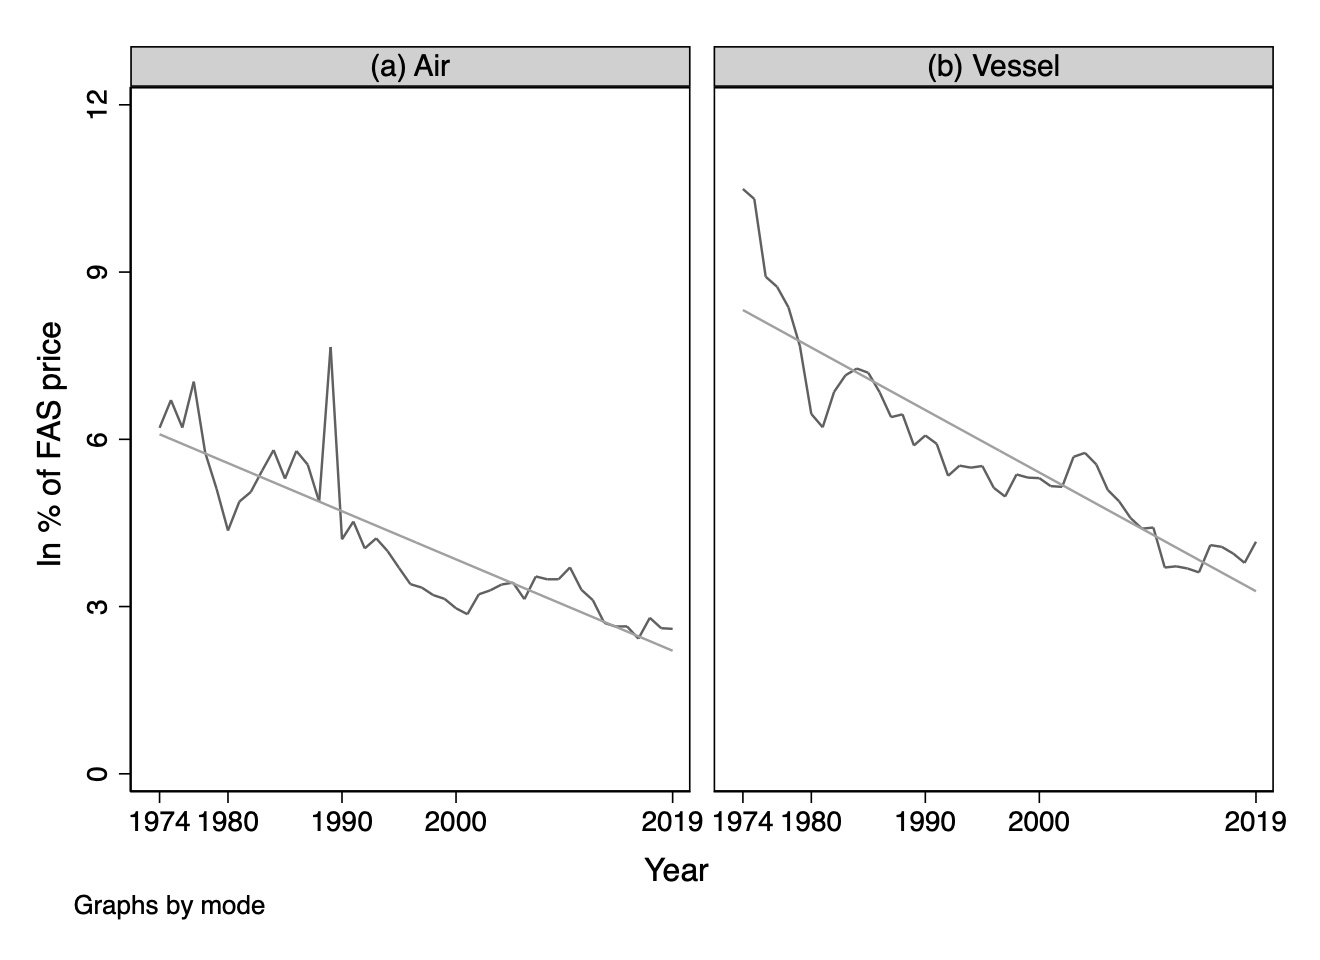
\includegraphics[width=14cm, height=7cm]{Figure2_Trend_of_totalTC_bymode.jpg}

\begin{minipage} [c]  {5in} \scriptsize%
Notes: We use the yearly values of the estimated transport cost components averaged over the country/product dimensions (at the 3-digit level). Each yearly value is obtained as: $\widehat{\tau}-1+\frac{\widehat{t}}{\widetilde{p}}$. 1989 trade by air is excluded.
\end{minipage}
\end{center}
\end{figure}

%%Sur le trend :      +------------------------------+
%| trend_~t         mode   year |
%|------------------------------|
%1. | 3.652468   (b) Vessel   2019 |
%46. | 8.546226   (b) Vessel   1974 |
%47. | 2.488636      (a) Air   2019 |
%92. | 6.289694      (a) Air   1974 |
%+------------------------------+



As shown in Figure \ref{fig:Trends_in_TC}, both air and vessel shipping exhibit a downward trend in overall transport costs since 1974, by -2.1\% per year for mean air transport costs and -1.9\% for mean vessel transport costs, implying a 60\% decrease in both air and vessel over the period.\footnote{One may be puzzled by the high magnitude of estimates for the beginning of the period (until 1980 approximately) for vessel transport.
\cite{hummels2007} finds similar outcomes on tramp prices indexes, and suggests the oil shock as a likely culprit, in a context where technological progress was quicker in aviation than in vessel, allowing a better dampening of oil shocks on air freight rates.
In a related manner, one may worry that the strong decrease in transport costs documented in Figure \ref{fig:Trends_in_TC} springs from high oil-shock-related transport costs in 1974. However, computing the time trends from 1980 does not dramatically change the picture.
The yearly trend from 1980 is -2\% for mean air transport costs and -1.6\% for mean vessel transport costs.
We thus choose to exploit the whole time dimension of our database by taking 1974 as starting date of our time-trend analysis.} 

%Using US data, \cite{Hummels_1999} found that overall transport cost declined from 6\% to 4\% of the import value between 1974 and 1996.
%For the same years, we obtain a total decrease from 5.3\% to 3\% in terms of the export price on average for air shipping, and from 8.9\% to 4.6\% for ocean shipping. Overall, our results display trends confirm and extend those reported by \cite{Hummels_1999} up to the very recent years.\smallskip

\paragraph{The share of additive costs: Time dynamics} Figure \ref{fig:part_cout_additif} reports the share of additive costs in total transport costs on a yearly basis, in both air and vessel transport, based on the weighted-mean values $\widehat{t}/\widetilde{p}$ and $\widehat{\tau}$.

\begin{figure}[htbp]
\caption{Share of additive costs $\beta$ (baseline at 3-digit level)}
\label{fig:part_cout_additif}
\begin{center}
 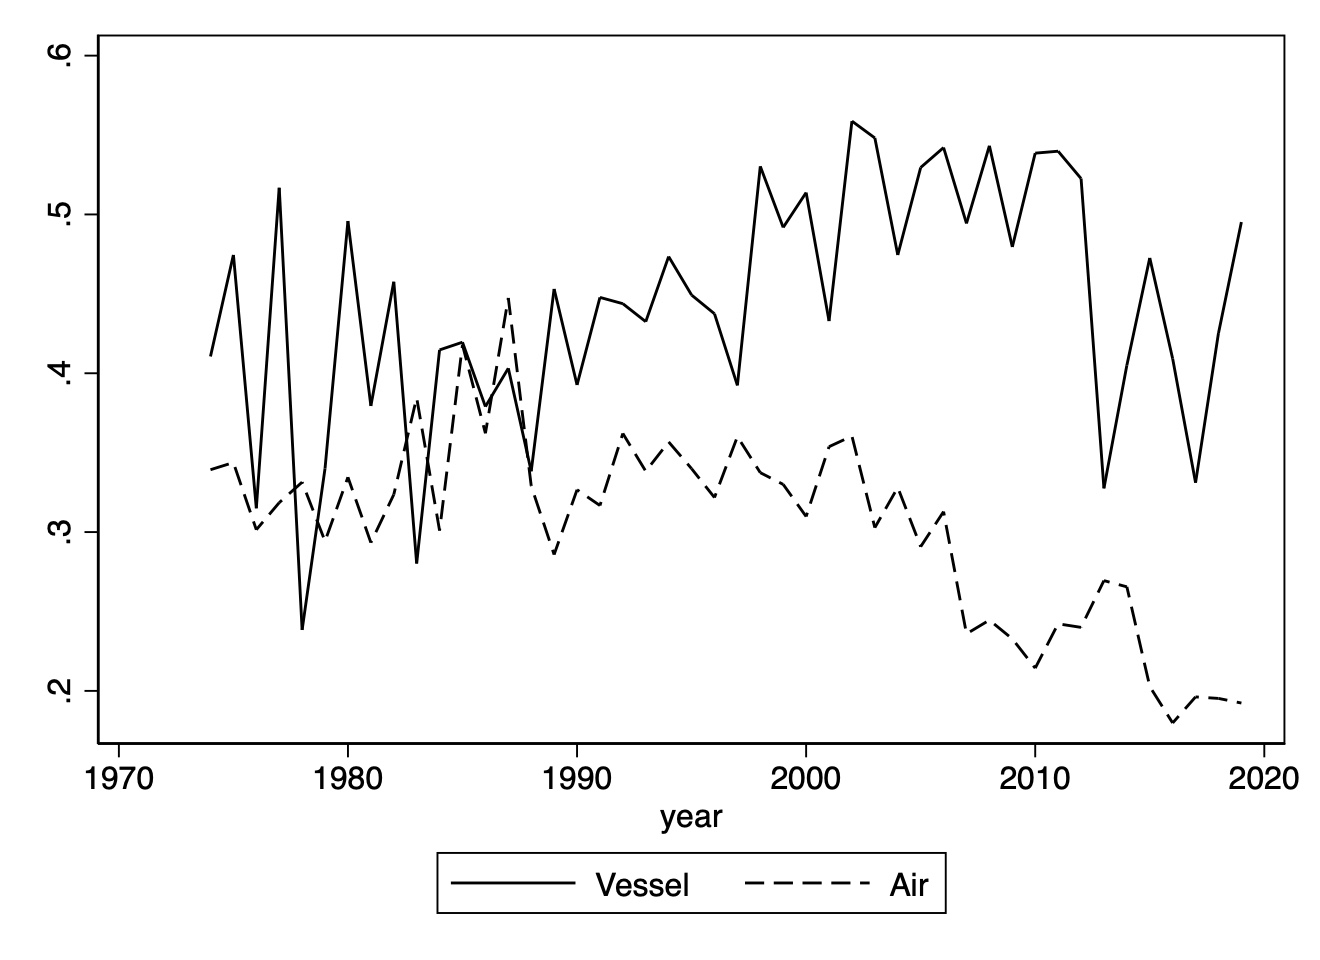
\includegraphics[width=12cm, height=7.5cm]{Figure1_share_of_additive_in_totalTC.jpg}
%{\footnotesize {OECD data} }
\begin{minipage} [c]  {5in} \scriptsize%
Note: The dotted line is the quadratic trend.
\end{minipage}
\end{center}
\end{figure}


%Le beta sur le trend quadratic (  reg ln_meanshareA year year2 )
%
%   +------------------------------+
%| trend_~a         mode   year |
%|------------------------------|
%1. |  .438216   (b) Vessel   2019 |
%46. | .3468959   (b) Vessel   1974 |
%47. | .2301836      (a) Air   2019 |
%92. | .3839365      (a) Air   1974 |
%+------------------------------+
%))


In both transport modes, the additive component appears of sizable importance throughout the period.
Confirming the results obtained in Table \ref{tab:summary_results}, this suggests that additive costs play a substantial role in total transport costs throughout the period. If the share of additive costs in total costs roughly amounts to 44\% (30\%) in vessel (air) transport on average, one can further notice that it varies substantially over time, with a different pattern across transport modes. After a period of common increase in air and vessel from the mid 1970s to the end of the 1980s, it has steadily decreased for air transport. In contrast, the share of additive costs has continued to increase until the 2000s. Put differently, the total transport costs decrease is more than proportionally due to additive costs in air transport, while it is mostly driven by ad-valorem cost reduction in vessel transport.\smallskip

In the following section, we check the robustness of these results regarding three important issues, the separability assumption of country-good fixed effects, potential endogeneity biases and the level of aggregation at the product level.

\subsection{Robustness analysis \label{sec:robustness}}


\subsubsection{Robustness to the separability assumption}
Following \cite{Irrazabal_2015}, we have assumed that both the ad-valorem and the additive costs are separable between the origin country ($i$) and the sector ($s(k)$) dimensions. In this section, we provide a robustness analysis to this separability assumption. That is, we relax Equations (\ref{eq:ad-valorem}) and (\ref{eq:add}) to model $\tau_{is(k)}$ and $t_{is(k)}$ (on a yearly/transport mode basis). This comes at the cost of having to estimate a much larger number of fixed effects (for approx. 200 countries of origin and 200 sectors at the 3-digit level, this means estimating 40,000 versus 400 fixed effects, per year and per transport mode), making the estimation intractable in practice (all the more given our non-linear setting).
This drives us to conduct the analysis on a sub-sample of trade flows, upon which two estimations are conducted (for every year and each transport mode): with the separability assumption (Equations (\ref{eq:ad-valorem}) and (\ref{eq:add}) hold, our baseline case) and without.
For each year and transport mode, we select the countries ($i$) and the products (at the 3-digit level, $s(k)$) that constitute 80\% of the total value of trade flows. Table \ref{tab:robustness_separability} shows a summary of the results, considering the average estimated values over the period (by transport mode).
%\textbf{LP: Pb avec le nb d'observations. } GD : CELA A L’AIR BON ET ON LAISSE COMME CELA
%
%\begin{table}[htbp]
%  \centering
%  \caption{Robustness to the separability assumption (average over the period) - restricted sample}
%\begin{center}
%    \begin{tabular}{lcc|cc}
%    \hline \hline
%    \multicolumn{5}{c}{Mean value over 1974-2019} \\
% \multicolumn{5}{c}{3 digits} \\    \hline \hline
%   Mode  & \multicolumn{2}{c|}{Air} & \multicolumn{2}{c}{Vessel} \\ \hline
%   Separability & No  & Yes (baseline) & No & Yes (baseline)\\ \hline
%    \multicolumn{5}{l}{\textit{Additive term} ($\widehat{t}/\widetilde{p}$.
%in \%)}  \\
%    Mean  & 1.76 & 1.96 & 2.61 & 2.99 \\
%    Median &0.65 & 0.84 &1.83 & 2.23 \\ \hline
%    \multicolumn{5}{l}{\textit{Ad-valorem term} ($\widehat{\tau}$, in \%)}\\
%    Mean  & 1.04 & 0.94 & 2.43 & 2.40 \\
%    Median & 0.56 & 0.83 & 2.06 & 2.04 \\ \hline
%\multicolumn{5}{l}{\textit{Share of additive costs in total costs (in \%)}} \\
%    Mean  & 62.8  & 67.5  & 51.8  & 55.4 \\
%    Median & 54.1  & 50.5  & 47.0  & 52.2 \\  \hline
% \textit{Diagnostic test} & & &  &  \\
%    %$R^2$    & \multicolumn{1}{c}{0.80} & \multicolumn{1}{c}{0.68} & \multicolumn{1}{c}{0.67} & \multicolumn{1}{c}{0.45} \\
%    %SER   & \multicolumn{1}{c}{0.57} & \multicolumn{1}{c}{0.72} & \multicolumn{1}{c}{0.53} & \multicolumn{1}{c}{0.69} \\
%    AIC criteria & 4657.60 & 4654.23 & 10744.83 & 10690.80 \\ \hline
%    %Log-likelihood & \multicolumn{1}{c}{-1757.75} & \multicolumn{1}{c}{-2258.24} & \multicolumn{1}{c}{-4018.51} & \multicolumn{1}{c}{-5220.00} \\ \hline
%\# observations & 2381 & 2381 & 2798 & 2798 \\
%\# origin country & 13.4 & 13.4 & 19.8 & 19.8 \\
%\# products & 25.5 & 25.5 & 53 & 53 \\ \hline \hline
%    \end{tabular}%
%\end{center}
%\parbox[l]{12cm}{\footnotesize{Notes: Estimations are performed on a restricted sample, based on the following rule: for each year and transport mode, we select the countries ($i$) and the products (at the 3-digit level, $s(k)$) that constitute 80\% of the total value of trade flows.
%The additive term is expressed in fraction of fas price. 1989 omitted in 3-digit estimation for air.}}
%\label{tab:robustness_separability}
%\end{table}

\begin{table}[htbp]
	\centering
	\caption{Robustness to the separability assumption - restricted sample}
	\begin{center}
			\begin{tabular}{l|cccc}
\cline{1-5}
\multicolumn{1}{l}{Transport mode} &
  \multicolumn{2}{|c}{Air} &
  \multicolumn{2}{|c}{Vessel} \\
\cline{1-5}
\multicolumn{5}{l}{\textbf{Data}} \\ \hline
%\multicolumn{5}{l}{\hspace{1em}Mean}  \\
\multicolumn{1}{l|}{\hspace{2em}{$\#$ obs.}} &
  \multicolumn{2}{c|}{2,125} &
  \multicolumn{2}{c}{5,260} \\
\multicolumn{1}{l|}{\hspace{2em}{$\#$ sectors}} &
  \multicolumn{2}{c|}{25} &
  \multicolumn{2}{c}{54}  \\
\multicolumn{1}{l|}{\hspace{2em}{$\#$ origin countries}} &
  \multicolumn{2}{c|}{14} &
  \multicolumn{2}{c}{20} \\ \hline
  \multicolumn{5}{l}{{\textbf{Estimations}}}  \\ \hline
  \multicolumn{1}{l}{Separability} &
  \multicolumn{1}{|c}{Yes (Baseline)} &
  \multicolumn{1}{c}{No} &
  \multicolumn{1}{|c}{Yes (Baseline)} &
  \multicolumn{1}{c}{No} \\ \hline
\multicolumn{5}{l}{\hspace{1em}{\textit{Multiplicative term, in $\%$} ($\widehat{\tau}^{adv}-1$)}}  \\ \hline
\multicolumn{1}{l}{\hspace{2em}Mean} &
  \multicolumn{1}{|c}{0.9} &
  \multicolumn{1}{c}{1.0} &
  \multicolumn{1}{|c}{2.3} &
  \multicolumn{1}{c}{2.3} \\
\multicolumn{1}{l}{\hspace{2em}Median} &
  \multicolumn{1}{|c}{0.7} &
  \multicolumn{1}{c}{0.5} &
  \multicolumn{1}{|c}{1.7} &
  \multicolumn{1}{c}{1.9} \\ \hline
\multicolumn{5}{l}{\hspace{1em}{\textit{Additive term, in $\%$} ($\widehat{t}/\widetilde{p}$)}}  \\ \hline
\multicolumn{1}{l}{\hspace{2em}Mean} &
  \multicolumn{1}{|c}{1.8} &
  \multicolumn{1}{c}{1.6} &
  \multicolumn{1}{|c}{2.9} &
  \multicolumn{1}{c}{2.5} \\
\multicolumn{1}{l}{\hspace{2em}Median} &
  \multicolumn{1}{|c}{0.7} &
  \multicolumn{1}{c}{0.6} &
  \multicolumn{1}{|c}{2.1} &
  \multicolumn{1}{c}{1.7} \\ \hline
\multicolumn{5}{l}{\hspace{1em}$\widehat{\beta}$:  \textit{Share of additive costs}}  \\ \hline
\multicolumn{1}{l}{\hspace{2em}Mean} &
  \multicolumn{1}{|c}{0.48} &
  \multicolumn{1}{c}{0.52} &
  \multicolumn{1}{c}{0.55} &
  \multicolumn{1}{c}{0.49} \\
\multicolumn{1}{l}{\hspace{2em}Median} &
  \multicolumn{1}{|c}{0.51} &
  \multicolumn{1}{c}{0.55} &
  \multicolumn{1}{|c}{0.58} &
  \multicolumn{1}{c}{0.48} \\ \hline
\multicolumn{1}{l}{\hspace{1em}AIC} &
%\multicolumn{1}{l}{\hspace{1em}Mean} &
  \multicolumn{1}{|c}{4,841} &
  \multicolumn{1}{c}{4,857} &
  \multicolumn{1}{|c}{12,053} &
  \multicolumn{1}{c}{12,154} \\
\cline{1-5}
\end{tabular}

%			\begin{tabular}{lllll}
\cline{1-5}
\multicolumn{1}{c}{} &
  \multicolumn{2}{|c}{air} &
  \multicolumn{2}{c}{ves} \\
\multicolumn{1}{c}{} &
  \multicolumn{1}{|r}{baseline} &
  \multicolumn{1}{r}{wo separability} &
  \multicolumn{1}{r}{baseline} &
  \multicolumn{1}{r}{wo separability} \\
\cline{1-5}
\multicolumn{1}{l}{\textbf{Data}} &
  \multicolumn{1}{|r}{} &
  \multicolumn{1}{r}{} &
  \multicolumn{1}{r}{} &
  \multicolumn{1}{r}{} \\
\multicolumn{1}{l}{\hspace{1em}Mean} &
  \multicolumn{1}{|r}{} &
  \multicolumn{1}{r}{} &
  \multicolumn{1}{r}{} &
  \multicolumn{1}{r}{} \\
\multicolumn{1}{l}{\hspace{2em}{$\#$ obs.}} &
  \multicolumn{1}{|r}{2,125} &
  \multicolumn{1}{r}{2,125} &
  \multicolumn{1}{r}{5,260} &
  \multicolumn{1}{r}{5,260} \\
\multicolumn{1}{l}{\hspace{2em}{$\#$ sectors}} &
  \multicolumn{1}{|r}{25} &
  \multicolumn{1}{r}{25} &
  \multicolumn{1}{r}{54} &
  \multicolumn{1}{r}{54} \\
\multicolumn{1}{l}{\hspace{2em}{$\#$ origin countries}} &
  \multicolumn{1}{|r}{14} &
  \multicolumn{1}{r}{14} &
  \multicolumn{1}{r}{20} &
  \multicolumn{1}{r}{20} \\
\multicolumn{1}{l}{{\textbf{Estimations}}} &
  \multicolumn{1}{|r}{} &
  \multicolumn{1}{r}{} &
  \multicolumn{1}{r}{} &
  \multicolumn{1}{r}{} \\
\multicolumn{1}{l}{\hspace{1em}{\textit{Multiplicative term (in $\%$)} ($\widehat{\tau}^{adv}$)}} &
  \multicolumn{1}{|r}{} &
  \multicolumn{1}{r}{} &
  \multicolumn{1}{r}{} &
  \multicolumn{1}{r}{} \\
\multicolumn{1}{l}{\hspace{2em}Mean} &
  \multicolumn{1}{|r}{0.9} &
  \multicolumn{1}{r}{1.0} &
  \multicolumn{1}{r}{2.3} &
  \multicolumn{1}{r}{2.3} \\
\multicolumn{1}{l}{\hspace{2em}Median} &
  \multicolumn{1}{|r}{0.7} &
  \multicolumn{1}{r}{0.5} &
  \multicolumn{1}{r}{1.7} &
  \multicolumn{1}{r}{1.9} \\
\multicolumn{1}{l}{\hspace{1em}{\textit{Additive term (in $\%$)} ($\widehat{t}/\widetilde{p}$)}} &
  \multicolumn{1}{|r}{} &
  \multicolumn{1}{r}{} &
  \multicolumn{1}{r}{} &
  \multicolumn{1}{r}{} \\
\multicolumn{1}{l}{\hspace{2em}Mean} &
  \multicolumn{1}{|r}{1.8} &
  \multicolumn{1}{r}{1.6} &
  \multicolumn{1}{r}{2.9} &
  \multicolumn{1}{r}{2.5} \\
\multicolumn{1}{l}{\hspace{2em}Median} &
  \multicolumn{1}{|r}{0.7} &
  \multicolumn{1}{r}{0.6} &
  \multicolumn{1}{r}{2.1} &
  \multicolumn{1}{r}{1.7} \\
\multicolumn{1}{l}{\hspace{1em}$\widehat{\beta}$:  \textit{-Share of additive costs}} &
  \multicolumn{1}{|r}{} &
  \multicolumn{1}{r}{} &
  \multicolumn{1}{r}{} &
  \multicolumn{1}{r}{} \\
\multicolumn{1}{l}{\hspace{2em}Mean} &
  \multicolumn{1}{|r}{-0.48} &
  \multicolumn{1}{r}{-0.52} &
  \multicolumn{1}{r}{-0.55} &
  \multicolumn{1}{r}{-0.49} \\
\multicolumn{1}{l}{\hspace{2em}Median} &
  \multicolumn{1}{|r}{-0.51} &
  \multicolumn{1}{r}{-0.55} &
  \multicolumn{1}{r}{-0.58} &
  \multicolumn{1}{r}{-0.48} \\
\multicolumn{1}{l}{{\textbf{AIC}}} &
  \multicolumn{1}{|r}{} &
  \multicolumn{1}{r}{} &
  \multicolumn{1}{r}{} &
  \multicolumn{1}{r}{} \\
\multicolumn{1}{l}{\hspace{1em}Mean} &
  \multicolumn{1}{|r}{4,841} &
  \multicolumn{1}{r}{4,857} &
  \multicolumn{1}{r}{12,053} &
  \multicolumn{1}{r}{12,154} \\
\cline{1-5}
\end{tabular}

	\end{center}
	\parbox[l]{12cm}{\footnotesize{Notes: Estimations are performed on a restricted sample, based on the following rule:  we select, for each year, the largest importers that form together at least 80\% of annual trade and the largest traded sectors that form together at least 80\% of annual trade. We keep in the sample all trade observations from these importers and in these sectors.
			The additive term is expressed in fraction of fas price.}}
	\label{tab:robustness_separability}
\end{table}

%use "/Users/guillaumedaudin/Documents/Recherche/2013 -- Trade Costs -- local/results/comparaisons_various/stats_comp_baseline_non_séparé.dta", clear
%gen cover = cover_non_séparé/cover_baseline
%sum coveruse "/Users/guillaumedaudin/Documents/Recherche/2013 -- Trade Costs -- local/results/comparaisons_various/stats_comp_baseline_non_séparé.dta", clear
%gen cover = cover_non_séparé/cover_baseline
%sum cover

Three main comments can be made. First, the subset of large trade flows we are considering (around 8\% of the observations of our initial sample, but the vast majority of the total value of aggregated trade, with an annual mean of 68\%) involve a higher share of additive costs: between 48\% and 55\% of total costs on average, versus 30\% to 44\% on the whole sample.
%JH: la phrase suivante est en contradiction avec celle qui suit encore juste après: "Second, assuming that country/product fixed effects are separable in these two dimensions tends to overestimate the value and the share of the additive costs."
Second, both models provide a similar quality of fit of the regression (once we take into account the number of right-hand-side variables) as the AIC criteria display very close values in both models (conditional on transport mode). Third, crucially for this robustness check the estimated values remain of similar magnitude under both separability and non-separability assumptions.\footnote{We also report in Section C from the Online Appendix a robustness check comparing the results with/without the separability assumption on a yearly basis} %, even if one can note that under the separability assumption, the share of additive costs seems slightly biased upward, at least for averages over the period. The picture is reversed for medians

\begin{figure}[htbp]
	\caption{Transport cost time trends: robustness to the separability assumption}
	\label{fig:comp_separability_SITC5}
	\begin{center}
		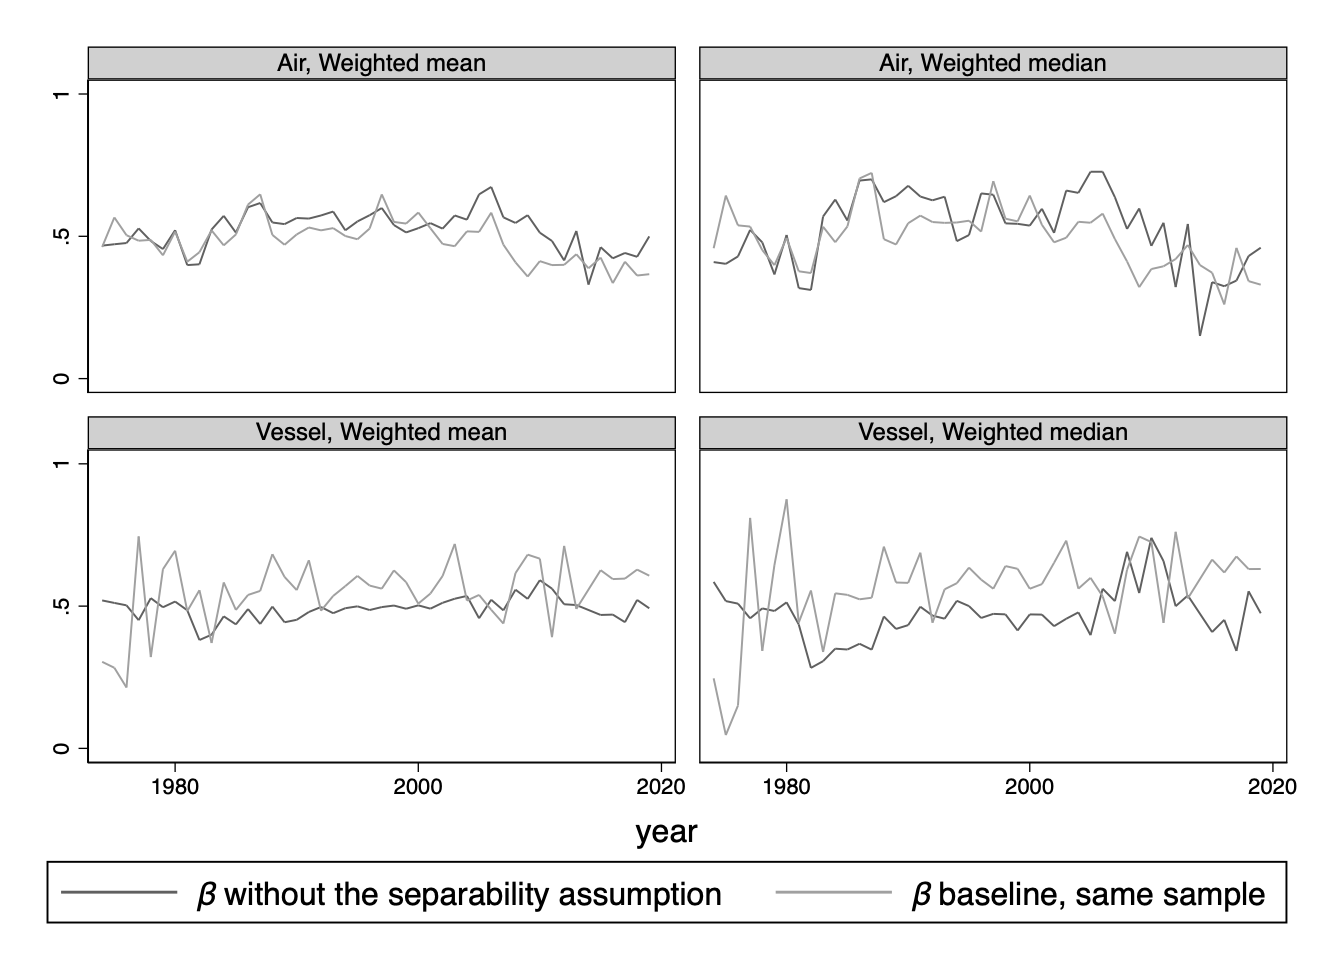
\includegraphics[height=8cm]
		{scatter_chronology_non_separe_pour_robustesse_ns.png}
	\end{center}
\end{figure}
%viens de comparaison.do



\subsubsection{Endogeneity concerns} One may be concerned that the specification of Equations (\ref{eq:model_IetA}) or (\ref{eq:model_nlI}) is subject to an endogeneity bias, as the price set by the exporter may vary depending on the transport cost burden. Studies on the pricing-to-market behavior of firms (see \citealp{Krugman-87}) show that we cannot exclude that the export price set by the firm ($\widetilde{p}_{ik}$) is partly endogenous to the size of transport costs (for instance, the exporting firm absorbing (part of) the transport costs by reducing the fas price).
Related concerns may arise from productivity-sorting model in \cite{melitz} or the quality-sorting model in \cite{baldwin_harrigan}: more productive firms and/or firms selling high-quality products will charge higher prices, all other things equal – in our case, for a given country-product pair. In addition, there is also the possibility that bigger firms might impact transport costs, due to their ability of bargaining discounts for larger shipped volumes.

It is true we are not interested in causal inference, since our aim is to provide an accounting breakdown of transport costs between the additive and the multiplicative components. However, the latter can be biased by the aforementioned endogeneity issues since they imply that $\frac{1}{\widetilde{p}_{ik}}$ is correlated in one direction on another with residuals $\epsilon_{ik}$. This may ultimately harm the estimation of $\widehat{t}/\widetilde{p}$ and consequently, $\widehat{\tau}$.

Therefore, we propose to compare our main estimates with those stemming from a two-stage least-squares procedure. We follow earlier literature (see e.g. \citealp{Caliendo_Parro_2015} or \citealp{Lashkaripour-2017}) by replacing in the right-hand side of Equation (\ref{eq:model_IetA}) $\widetilde{p}$ by predicted values stemming from a first-stage equation regressing $\widetilde{p}$ on custom duties coming based on tariffs at the product line, together with one-year lagged fas prices. Section \ref{app:first_stage_IV} in Appendix \ref{app:more_results} provides a full presentation of the theoretical basis for the first-stage equation, as well as first-stage estimates. In particular, it shows that our main instrumental variable displays the right statistical properties, and that we can confidently re-inject the predictions arising from the first-stage equation for $\widetilde{p}_{ik}$ on the right-hand side of Equation (\ref{eq:model_IetA}) %\footnote{Note that, since the predictions are expressed in logarithms, they are transformed through the exponential function before their implementation in Equation (\ref{eq:model_IetA}.}
 to produce a 2SLS-type of estimation. Figure \ref{fig:comp_IV_SITC5} reports our benchmark estimates by transport mode, together with their instrumented counterpart. In all cases, these estimates are very similar, when not identical. This supports that our benchmark estimates do not suffer any substantial biases arising from endogeneity concerns.

\begin{figure}[htbp]
\caption{Transport cost time trends: robustness to IV procedure}
\label{fig:comp_IV_SITC5}
\begin{center}
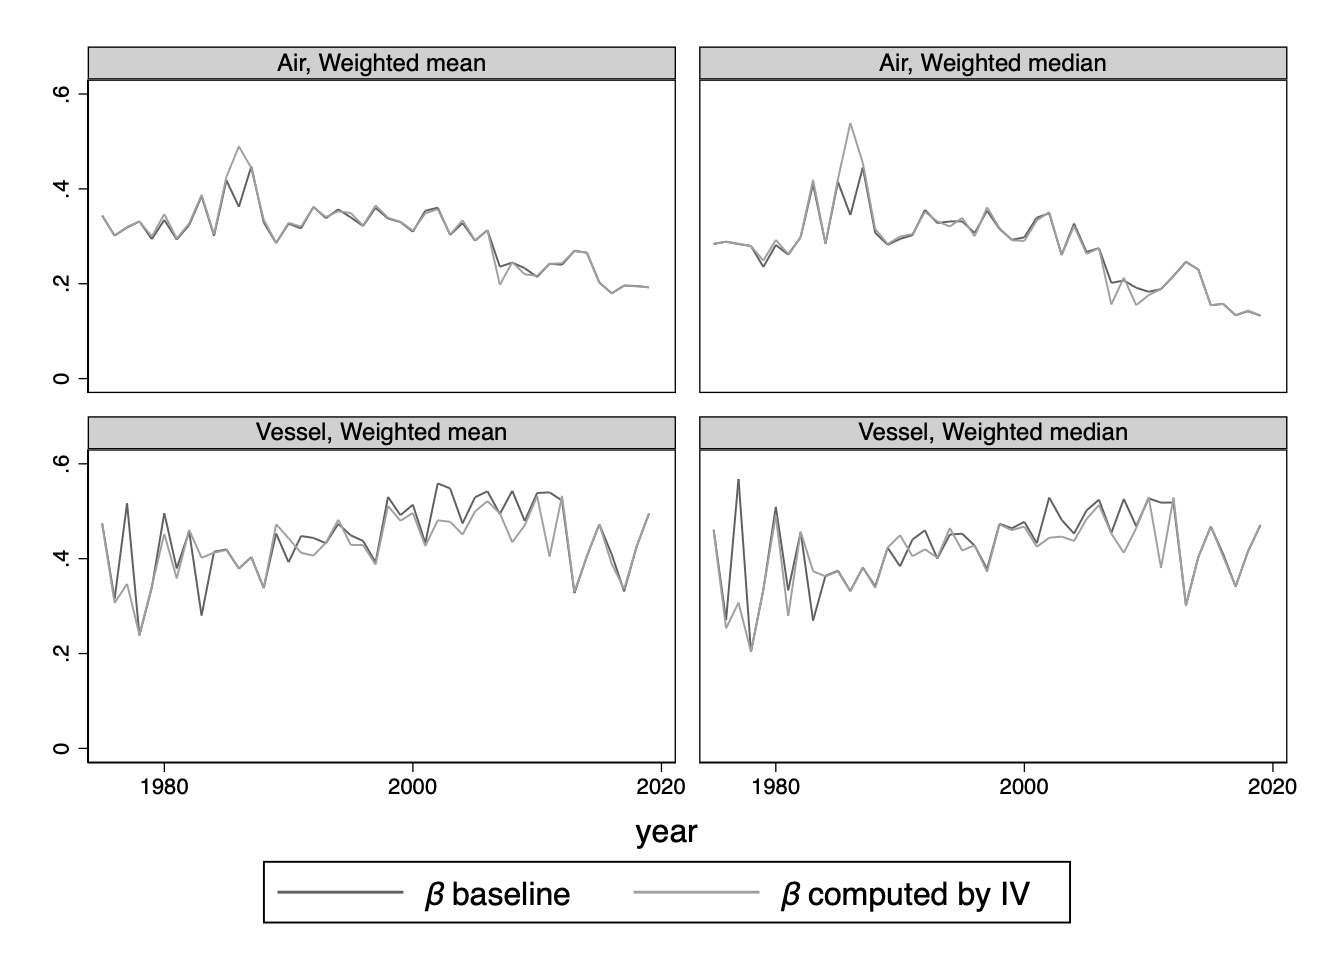
\includegraphics[height=8cm]
{scatter_chronology_baseline_IV_ref1_y_5_3.png}
\end{center}
\end{figure}
%viens de comparaison.do

%However, we consider as a reasonable assumption that the exporting firm cannot influence the international transport cost sector, that would imply a causal effect of the firm's prices on the transport costs value, except in the choice between air and vessel transport (that is beyond our scope of analysis).
%Otherwise stated, conditional to an export price and a transport mode, the gap between the export price declared to the custom data and the import price recorded by the US administration is beyond the firm's control.
%In this respect, we are confident that our estimation strategy is immune from endogeneity problems.


\subsubsection{Robustness to aggregation}

Current data are available at the 10-digit level for products (HS10) for some specific years. The results reported here rely on exploiting data from 2005 to 2019. This period is obviously smaller than our main sample, due to two main issues. Firstly, we could only access the years 1997-1999 and 2001-2019.\footnote{Theoretically, they should be available from 1989, which is already smaller than our full sample starting in 1974. Because of the COVID situation, it was only possible to get access to the years 1997-1999 and 2001-2019.} Secondly, for the years 1997-1999 and 2001-2005, compatibility issues between Census and Hummels' data prevented reliable comparisons.


Notice that switching to a 3 (sector)-10(product) estimation method does not alter the number of fixed effects to estimate, as they are at the sector $s$ level (along with those at the origin country $i$ level). However, within each 3-digit sector category, the 3-10 estimation method has the advantage to exploit a larger source of heterogeneity by considering trade flows at the HS-10 product level.

Yet, as Table \ref{tab:baseline10} and 	Figure \ref{fig:robustness_to_agregation} show, the results are very similar when using 10-digit product and 5-digit products. If anything, the $\beta$ seems on average slightly higher when estimated based on a 3 (sector)-10 (product) database, indicating a (small) downward bias in our estimates of additive costs. But overall, no major difference arises both regarding levels and trends - results are especially very close for the Air transportation mode. This has important implications for the exercise performed in Section \ref{sec:theory}: welfare gains computations should not be significantly affected by our use of 3 (sector)-5 (product) digit data. This is consistent with e.g. \citet{Giri_et_al2021}, who show that sectoral heterogeneity does not always lead to an increase in the gains from trade.

\begin{table}[htbp]
	\centering
	\caption{Transport costs estimates: Robustness to aggregation (2005-2019)} \vspace{5mm} \label{tab:baseline10}
	\begin{tabular}{l|cc|cc}
\cline{1-5}
\multicolumn{1}{c}{} &
  \multicolumn{2}{|c}{Air } &
  \multicolumn{2}{c}{Vessel} \\
\multicolumn{1}{c}{} &
  \multicolumn{1}{|c}{5-3 digit} &
  \multicolumn{1}{c}{10-3 digit} &
  \multicolumn{1}{c}{5-3 digit} &
  \multicolumn{1}{c}{10-3 digit} \\
\cline{1-5}
\multicolumn{1}{l}{\textbf{Data}} &
  \multicolumn{1}{|c}{} &
  \multicolumn{1}{c}{} &
  \multicolumn{1}{c}{} &
  \multicolumn{1}{c}{} \\ \hline
\multicolumn{1}{l}{\hspace{1em}Mean} &
  \multicolumn{1}{|c}{} &
  \multicolumn{1}{c}{} &
  \multicolumn{1}{c}{} &
  \multicolumn{1}{c}{} \\
\multicolumn{1}{l}{\hspace{2em}{$\#$ obs. ($k,i$)}} &
  \multicolumn{1}{|c}{24,910} &
  \multicolumn{1}{c}{172,470} &
    \multicolumn{1}{c}{22,722} &
  \multicolumn{1}{c}{150,153} \\
\multicolumn{1}{l}{\hspace{2em}{$\#$ sectors ($s$)}} &
  \multicolumn{2}{c}{174 \textbf{TBC}} &
  \multicolumn{2}{c}{\textbf{174 TBC}} \\
\multicolumn{1}{l}{\hspace{2em}{$\#$ origin countries}} &
  \multicolumn{1}{|c}{118} &
  \multicolumn{1}{c}{211} &
    \multicolumn{1}{c}{131} &
  \multicolumn{1}{c}{207} \\
\multicolumn{1}{l}{\hspace{1em}{\textit{Obs. transport costs $(p/\widehat{p}-1)$ (in $\%$)}}} &
  \multicolumn{1}{|c}{} &
  \multicolumn{1}{c}{} &
  \multicolumn{1}{c}{} &
  \multicolumn{1}{c}{} \\
\multicolumn{1}{l}{\hspace{2em}Mean} &
  \multicolumn{1}{|c}{2.9} &

  \multicolumn{1}{c}{2.9} &
    \multicolumn{1}{c}{4.3} &
  \multicolumn{1}{c}{4.2} \\
\multicolumn{1}{l}{\hspace{2em}Median} &
  \multicolumn{1}{|c}{1.7} &

  \multicolumn{1}{c}{1.5} &
    \multicolumn{1}{c}{3.2} &
  \multicolumn{1}{c}{3.1} \\
\multicolumn{1}{l}{\hspace{2em}Std. dev.} &
  \multicolumn{1}{|c}{4.7} &

  \multicolumn{1}{c}{5.0} &
    \multicolumn{1}{c}{3.7} &
  \multicolumn{1}{c}{4.0} \\
\multicolumn{1}{l}{\hspace{1em}{\textit{Export price in USD per kg (\textit{$\widehat{p}$})}}} &
  \multicolumn{1}{|c}{} &
  \multicolumn{1}{c}{} &
  \multicolumn{1}{c}{} &
  \multicolumn{1}{c}{} \\
\multicolumn{1}{l}{\hspace{2em}Mean} &
  \multicolumn{1}{|c}{12,843} &

  \multicolumn{1}{c}{11,749} &
    \multicolumn{1}{c}{11} &
  \multicolumn{1}{c}{16} \\
\multicolumn{1}{l}{\hspace{2em}Median} &
  \multicolumn{1}{|c}{205} &

  \multicolumn{1}{c}{267} &
    \multicolumn{1}{c}{4} &
  \multicolumn{1}{c}{4} \\
\multicolumn{1}{l}{\hspace{2em}Std. dev.} &
  \multicolumn{1}{|c}{50,529} &

  \multicolumn{1}{c}{54,665} &
    \multicolumn{1}{c}{521} &
  \multicolumn{1}{c}{572} \\ \hline
\multicolumn{1}{l}{{\textbf{Model (B)}}} &
  \multicolumn{1}{|c}{} &
  \multicolumn{1}{c}{} &
  \multicolumn{1}{c}{} &
  \multicolumn{1}{c}{} \\
\multicolumn{1}{l}{\hspace{1em}{\textit{Multiplicative term, in $\%$} ($\widehat{\tau}^{adv} -1$)}} &
  \multicolumn{1}{|c}{} &
  \multicolumn{1}{c}{} &
  \multicolumn{1}{c}{} &
  \multicolumn{1}{c}{} \\
\multicolumn{1}{l}{\hspace{2em}Mean} &
  \multicolumn{1}{|c}{2.0} &

  \multicolumn{1}{c}{2.6} &
    \multicolumn{1}{c}{45.7} &
  \multicolumn{1}{c}{2.7} \\
\multicolumn{1}{l}{\hspace{2em}Median} &
  \multicolumn{1}{|c}{1.5} &

  \multicolumn{1}{c}{2.2} &
    \multicolumn{1}{c}{10.8} &
  \multicolumn{1}{c}{2.5} \\
\multicolumn{1}{l}{\hspace{2em}Std. dev.} &
  \multicolumn{1}{|c}{2.1} &

  \multicolumn{1}{c}{2.0} &
    \multicolumn{1}{c}{50.7} &
  \multicolumn{1}{c}{1.4} \\
\multicolumn{1}{l}{\hspace{1em}{\textit{Additive term, in $\%$} ($\widehat{t}/\widetilde{p}$)}} &
  \multicolumn{1}{|c}{} &
  \multicolumn{1}{c}{} &
  \multicolumn{1}{c}{} &
  \multicolumn{1}{c}{} \\
\multicolumn{1}{l}{\hspace{2em}Mean} &
  \multicolumn{1}{|c}{1.2} &

  \multicolumn{1}{c}{1.1} &
    \multicolumn{1}{c}{14.5} &
  \multicolumn{1}{c}{2.1} \\
\multicolumn{1}{l}{\hspace{2em}Median} &
  \multicolumn{1}{|c}{0.5} &

  \multicolumn{1}{c}{0.4} &
    \multicolumn{1}{c}{6.8} &
  \multicolumn{1}{c}{1.2} \\
\multicolumn{1}{l}{\hspace{2em}Std. dev.} &
  \multicolumn{1}{|c}{2.5} &
 
  \multicolumn{1}{c}{2.5} &
   \multicolumn{1}{c}{50.7} &
  \multicolumn{1}{c}{3.3} \\
\multicolumn{1}{l}{\hspace{1em}{\textit{Additive term in USD per kg ($\widehat{t}$)}}} &
  \multicolumn{1}{|c}{} &
  \multicolumn{1}{c}{} &
  \multicolumn{1}{c}{} &
  \multicolumn{1}{c}{} \\
\multicolumn{1}{l}{\hspace{2em}Mean} &
  \multicolumn{1}{|c}{1.51} &

  \multicolumn{1}{c}{1.23} &
    \multicolumn{1}{c}{0.47} &
  \multicolumn{1}{c}{0.10} \\
\multicolumn{1}{l}{\hspace{2em}Median} &
  \multicolumn{1}{|c}{1.40} &

  \multicolumn{1}{c}{1.14} &
    \multicolumn{1}{c}{0.15} &
  \multicolumn{1}{c}{0.10} \\
\multicolumn{1}{l}{\hspace{2em}Std. dev.} &
  \multicolumn{1}{|c}{1.04} &

  \multicolumn{1}{c}{0.74} &
    \multicolumn{1}{c}{0.47} &
  \multicolumn{1}{c}{0.08} \\
\multicolumn{1}{l}{\hspace{1em}$\widehat{\beta}$:  \textit{Share of additive costs}} &
  \multicolumn{1}{|c}{} &
  \multicolumn{1}{c}{} &
  \multicolumn{1}{c}{} &
  \multicolumn{1}{c}{} \\
\multicolumn{1}{l}{\hspace{2em}Mean} &
  \multicolumn{1}{|c}{0.38} &

  \multicolumn{1}{c}{0.20} &
    \multicolumn{1}{c}{0.44} &
  \multicolumn{1}{c}{0.37} \\
\multicolumn{1}{l}{\hspace{2em}Median} &
  \multicolumn{1}{|c}{0.39} &

  \multicolumn{1}{c}{0.14} &
    \multicolumn{1}{c}{0.41} &
  \multicolumn{1}{c}{0.36} \\
\multicolumn{1}{l}{\hspace{2em}Std. dev.} &
  \multicolumn{1}{|c}{0.15} &

  \multicolumn{1}{c}{0.19} &
    \multicolumn{1}{c}{0.29} &
  \multicolumn{1}{c}{0.21} \\
\cline{1-5}
\end{tabular}

	\begin{tablenotes}
		\scriptsize
		\item Statistics for 1997-1999 and 2002-2019
		\item Statistics are obtained weighting each observation by its value relative to total trade flows.
        \item Transport costs expressed in \% of the fas price (except for $\widehat{t}$ expressed in USD.
		%\item \textbf{Model (A): With ad-valorem transport costs only}
		\item Model (B): With additive and ad-valorem transport costs
	\end{tablenotes}
\end{table}


\begin{figure}[htbp]
	\caption{Transport cost time trends: Robustness to aggregation (2005-2019)}
	\label{fig:robustness_to_agregation}
	\begin{center}
		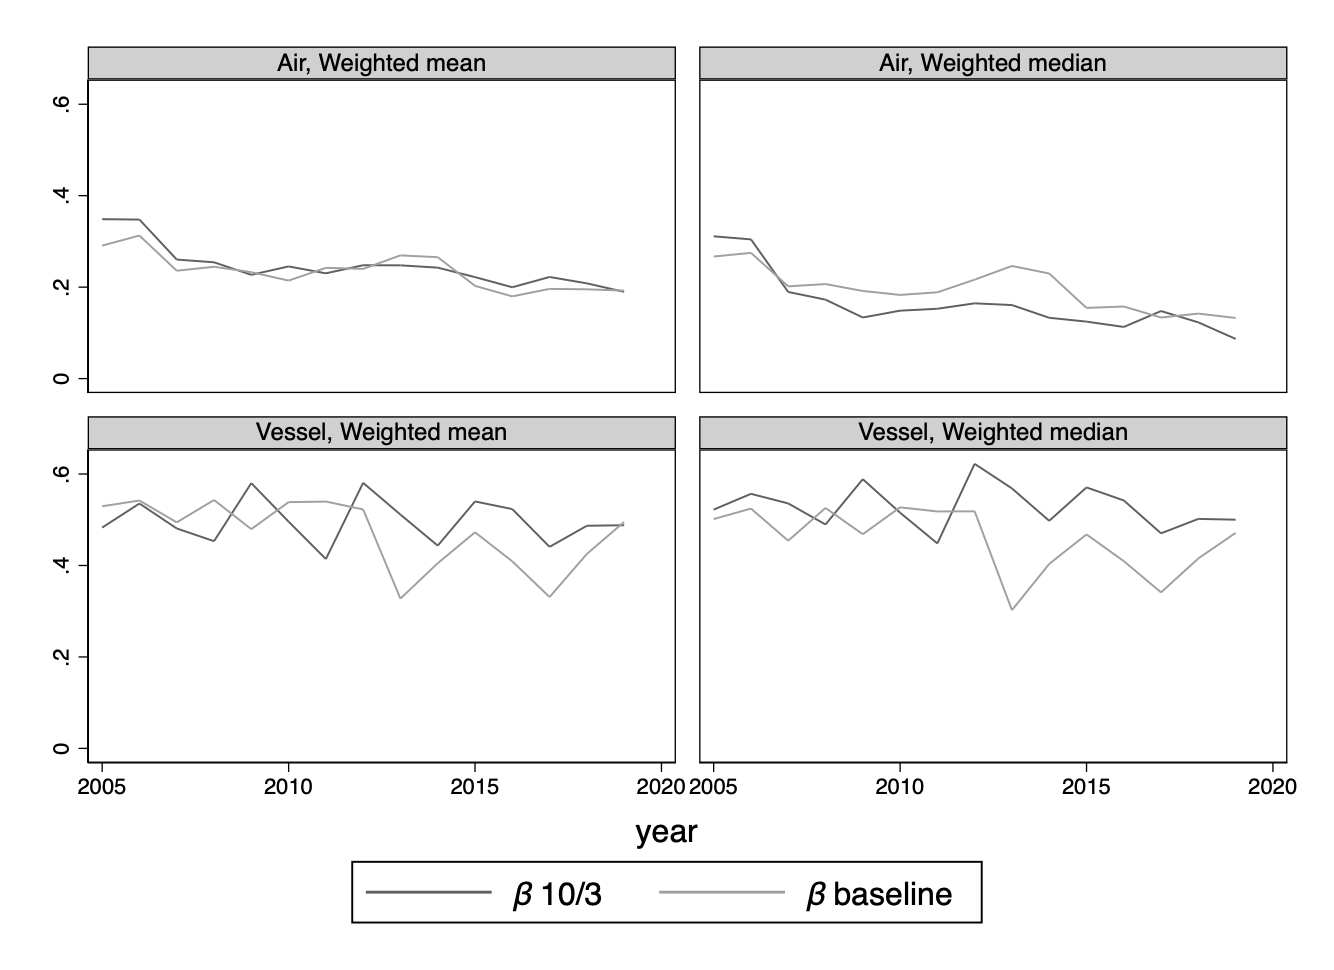
\includegraphics[height=8cm]{scatter_chronology_baseline10_dbsamesample10_5_3.png}
	\end{center}
\end{figure}


\paragraph{Summary} Two main insights emerge up to now. First, total transport costs have strongly reduced between 1974 and 2019. Second, additive costs represent an important share of those declining transport costs, between 30 and 45\%. In the two following sections, we take stock of those results to draw implications for two important debates in economic analysis. In the next section, we shed light on the origins of the decrease of transport costs over time, by providing a decomposition of the transport costs trend patterns, between what arises from changes in the trade composition (by product and/or partner country), and what is attributable to changes in transport costs \emph{per se}. Section \ref{sec:theory} implements several theory-based calibration exercises to investigate the different welfare consequences of alterations over time to multiplicative and additive costs.


\section{Transport costs time trends: the key part of additive costs}\label{sec:results_trends}

In this section, we investigate the underlying sources behind the downward trend of international transport costs, by identifying the respective roles of the reduction in ``pure'' transport costs and changes in trade composition effects. As underlined by \cite{hummels2007}, total transport costs may have decreased over time because the share of neighboring countries in total US trade or the share of goods cheaper to transport has increased (composition effects) independently of any change in transport costs \textit{per se}. It is hence necessary to eliminate the composition effects of trade flows to isolate the evolution of pure international transport costs. Specifically, \cites{hummels2007} results support that trade composition effects partially compensate the reduction in pure transport costs, thereby attenuating the downward trend in overall (observed) transport costs since 1974. Our own results tend to challenge this view, as we further show.

\paragraph{A word on Hummels' methodology} At this point, let us make a brief summary of Hummels' methodology\nocite{hummels2007}.
Starting from a similar specification as in Section \ref{sec:estimation_strat}, \cite{hummels2007} writes his transport cost measure $TC_{ikt}$ as:

\begin{equation}
TC_{ikt}\equiv \frac{p_{ikt}-\widetilde{p}_{ikt}}{\widetilde{p}_{ikt}} = \widetilde{p}_{ikt}^{-\beta}X_{ikt} \label{eq:Hummel_benchmarkeq}
\end{equation}

\noindent where $X_{ikt}$ represents other costs shifters (distance, port quality, etc.) and $\beta$ can be interpreted as the elasticity of transport costs to the export price (in absolute value), also equal to the share of additive costs in total transport costs.
Equation (\ref{eq:Hummel_benchmarkeq}) is the baseline specification from which \cite{hummels2007} decomposes the changes in transport costs over time between trade composition effects and changes in ``pure'' transport costs, as described in more detail in Appendix \ref{app:compare_Hummels}.
In doing so, \cite{hummels2007} implicitly assumes $\beta$ constant across the triplet origin country origin/product/year.
Put differently, this means that the share of additive costs in total costs does not vary across these dimensions.

\paragraph{Challenging the $\beta$'s constancy assumption} As Figure \ref{fig:part_cout_additif} suggests, the share of additive costs is rather varying over time, in both transport modes.
%In light of this, one may wonder about the constancy of the share of additive costs along the pair product/origin country hypothesized by \cite{hummels2007}.
We investigate this point deeper by reporting the histogram of the distribution of the share of additive costs in total costs.
To do so, we start from Equation (\ref{eq:base_estimee}) with the trade costs measure on the left-hand side, from which we deduce the formulae to get the elasticity of transport costs to the export price on a per product-year-country basis, i.e.
$\beta$, according to $\beta_{ikt} = \frac{\widehat{t}_{is(k)t}/\widetilde{p}_{ikt}}{\widehat{t}_{is(k)t}/\widetilde{p}_{ikt}+\widehat{\tau}_{is(k)t}-1},
$

\noindent making use of our first-stage estimates for both the additive and the ad-valorem components ($\widehat{t}_{is(k)t}$ and $\widehat{\tau}_{is(k)t}$). The histogram of the distribution of the estimated $\beta_{ikt}$ is reported in Figure \ref{fig:histogram_beta}, in panels (A) and (B) for air and maritime transport respectively.


\begin{figure}[htbp]
\caption{Share of additive costs in total costs: Histogram}
\label{fig:histogram_beta}
\begin{center}
\begin{tabular}{cc}
%{\small (A) Air } & {\small (B) Vessel}\\
\includegraphics[width=3.0in, height=2.5in]{"Etude_beta_pondere_(A) Air transport".jpg}
& \includegraphics[width=3.0in,height=2.5in]{"Etude_beta_pondere_(B) Vessel transport".jpg} \\
\multicolumn{2}{l}{{\footnotesize Notes: Distribution of $\beta_{ikt}$ over the triplet (year,product,country), weighted by share of yearly value of flow.}}\\
\end{tabular}
\end{center}
\end{figure}

As displayed in Figure \ref{fig:histogram_beta}, for both transport modes the distribution of $\beta_{ikt}$ over the triplet (year, product, origin country) is smoothly distributed over the interval $[0,1]$, with a mode of the distribution standing around 0.3-0.4 depending on the transport mode, consistently with our previous findings.
This stands in sharp contrast with the assumption made by  \cite{hummels_skiba} or \cite{hummels2007}, which would imply a distribution concentrated on a single point.
Rather, this suggests that the elasticity of transport costs to the export price, or equivalently the share of additive costs in total costs, is varying across time, product and country partner.\footnote{We have checked that it is also the case when we look at the distribution over the range of origin countries or products, for a given year.
These results are not reported for sake of space, but are available upon request to the authors.} In the next section, we shed light on the role of this result in the analysis of the underlying sources of the overall transport costs trend patterns, between trade composition effects and pure transport costs.

\subsection{Empirical specification}

Based on the above results, we provide a decomposition of the transport costs trends between the trade composition effects and the ``pure'' transport costs time trends, which explicitly takes into account the varying share of additive costs over time, country partner and product. We start with the presentation of our estimation strategy before turning to the results.

\subsubsection{Estimation strategy}

The estimation carried out in section \ref{sec:results_decomposition} provides us with the
Starting from the additive and ad-valorem measures of international transport costs which vary over time, product and origin country (i.e., $\widehat{t}_{ikt}$ and $\widehat{\tau}_{ikt}$), we extract the pure transport cost measure by the mean of a time fixed effect.
Precisely, we extract the changes over time in the pure transport cost dimension by assuming a composition of trade flows by country partner and product that is constant throughout the period, and equal to the one observed in 1974. We conduct the same analysis on an overall transport costs measure, built by combining the two estimated components (additive and ad-valorem) in a unified measure of transport costs. The objective is to obtain six time series, all built as indices with the reference value 100 in 1974: three time series for the unfitted transport costs measures $\{\Gamma^{t/\widetilde{p}, raw}_t, \Gamma^{adv, raw}_t, \Gamma^{tc, raw}_t \}$, and three series for the fitted values $\{\Gamma^{t/\widetilde{p}}_t, \Gamma^{adv}_t, \Gamma^{tc}_t \}$ (additive, ad-valorem and total cost respectively).

One advantage of this method is that it yields measures of transport costs (fitted and unfitted) that are easily comparable between transport modes and transport cost components.
For each cost component (additive and ad-valorem) as well as for the total transport cost, comparing the unfitted measure and the fitted measure (composition effects excluded) makes it possible to identify if the decrease observed over the period in the unfitted series is due to trade composition effects (for instance, changes in the country partners, in the type/quality of products traded), or if it is the pure transport costs (for instance, insurance or handling costs) that have reduced over time. For sake of reading clarity, we describe the method to extract these series in Appendix \ref{app:comp-effects}, and we now turn to the results.



\subsection{Characterizing the time trends in transport costs}
Figure \ref{fig:totalTC_compeffects_excl} reports the results for all types of goods.\footnote{In the Online Appendix, we report the results at a more disaggregated level, distinguishing between primary and manufacturing goods.} In panels (A), (B) and (c) we report the time changes of the ad-valorem costs, the additive costs and the total costs respectively, for air transport (starting from the reference value 100 in 1974).
Panels (d), (e) and (f) report the results for vessel.
In each panel, we report the evolution of transport costs for both the unfitted (plain blue line) and the fitted (dotted red line) measures.


\begin{figure}[htbp]
\caption{Transport costs (with and without composition effects)}
\label{fig:totalTC_compeffects_excl}
\begin{center}
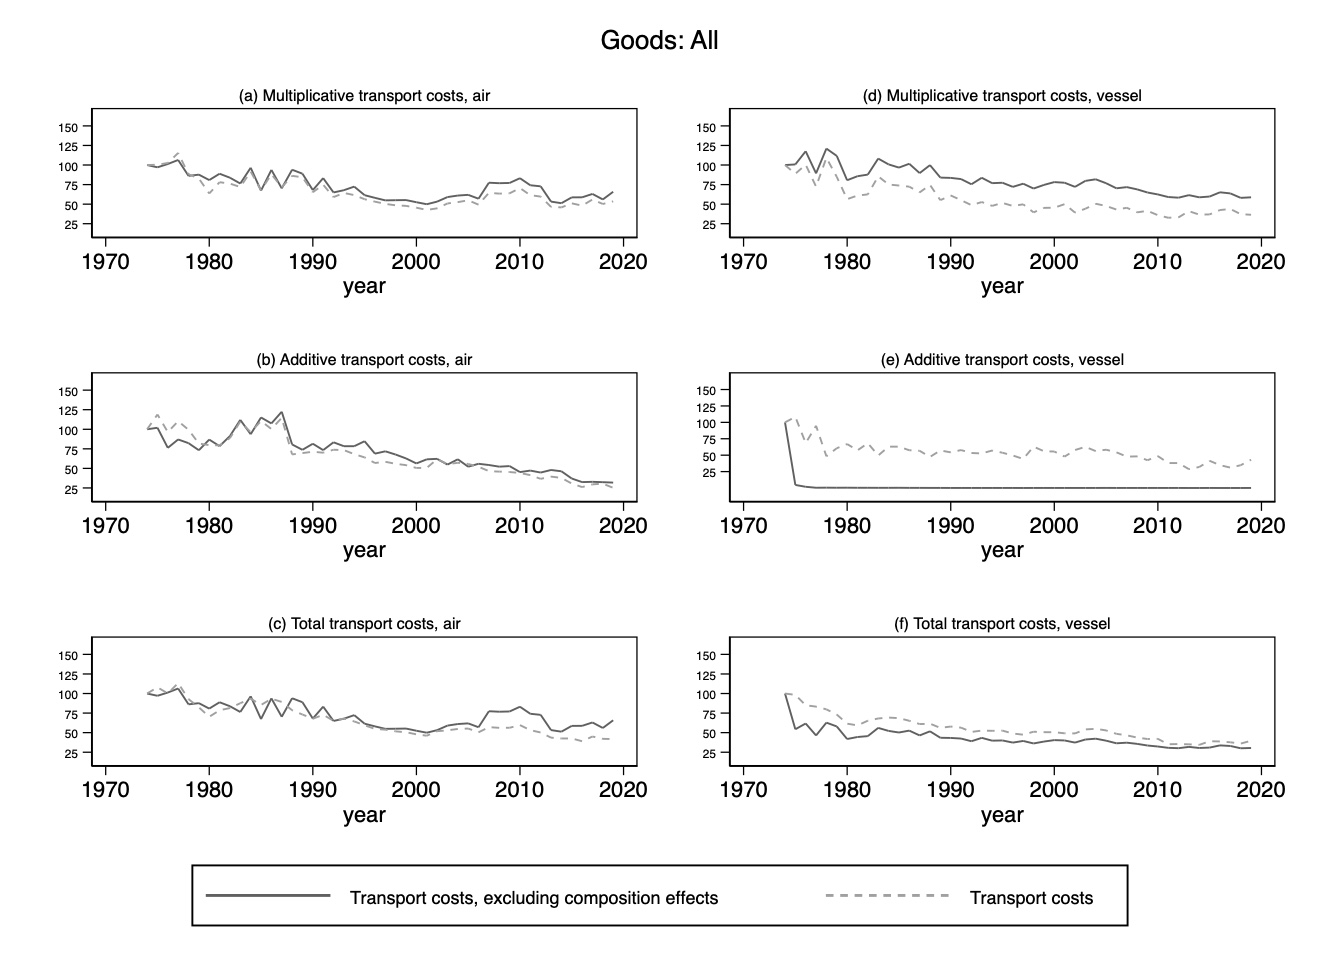
\includegraphics[height=4in]
{graph_composition_all.jpg}
\end{center}
\end{figure}

Three main results emerge from Figure \ref{fig:totalTC_compeffects_excl}.
First, in accordance with Figure \ref{fig:Trends_in_TC}, we find that international transport costs have substantially decreased over the period, for both transport modes (Panels (c) and (f)).
International transport costs were reduced by 50\% between 1974 and 2019 in air shipping, and by 60\% in maritime shipping. Second, the magnitude of the decrease is roughly of the same order for both for the ad-valorem and the additive components (Panels (a), (a), (d) and (e)).
Further, the transport cost reduction is much smoother in maritime transport, while air transport shows more volatility in the trend pattern, in particular in the 1980s and the 2000s.
Third, and most importantly, we find that composition effects do not play a major role in accounting for the time trend of overall transport costs.
Inspecting the panels of Figure \ref{fig:totalTC_compeffects_excl} for air transport (panels (A) to (c)), we do not find much evidence of a substantial trend difference between the unfitted transport costs measure and the pure transport costs.
For all three series (additive, ad-valorem and overall transport costs), the dotted and the plain line follow closely, almost every year throughout the period.
Air transport costs were reduced by 50\% between 1974 and 2019, which is mainly attributable to a reduction in the transport costs ``per se''.
Composition effects are stronger in vessel transport, for all three series (Figure \ref{fig:totalTC_compeffects_excl}, panels (d) to (f)): they amplify the reduction in ``pure'' transport costs at the beginning of the period, in the 1970s (the dotted line is below the plain line, and the gap is increasing). Afterwards, the gap between the two remains roughly constant across years, indicating that the amplification effect does not strengthen anymore: the two trends are similar.
Considering the raw series (plain line), maritime transport costs have decreased by 60\% over the period, which can be decomposed into a 50\% decrease in transport costs ``per se'' (dotted line), and a 10\% reduction that comes from composition effects (the difference of the two).
This is particularly the case for the multiplicative component (panel (d)).\smallskip


\subsection{Time trends in transport costs and the modeling of the additive component}

The last results stand in sharp contrast with \cite{hummels2007}, who finds that trade composition effects do matter, as they partially offset the reduction in the pure transport costs for both air and maritime shipping. If anything, we find the opposite result here: Trade composition effects do not matter much in accounting for the downward trend of observed international transport costs, and when they do, they tend to amplify (rather than reduce) the downward pattern. This drives us to investigate this difference further.

As we explain in more detail in Appendix \ref{app:comp-effects}, our empirical strategy differs from \cite{hummels2007} in one main dimension.
Rather than from the actual cif-fas price gap, we start from our estimates of both the additive and the ad-valorem components (obtained in Section \ref{sec:results_decomposition} at the year/sector/origin country level, by transport mode. Put differently, our methodology lets the share of additive costs $\beta$ vary over the three time-product-partner country dimensions. By contrast, \cite{hummels2007} does not take into account the changes in the additive transport cost component, attributing this to a change in the composition of the bundle over time (per country-commodity). This turns out to be of primary importance in the disentangling of the sources of the transport costs time trend. To establish this point clearly, we replicate the method adopted by \cite{hummels2007} exposed above on our database (which is the same as his until 2004). The results are reported in Figure \ref{fig:comp_effects_as_in_Hummels}. To ease the interpretation of the trends, we express them as indices with the reference value 100 in 1974, in Panels (c) and (d) for air and vessel respectively.\footnote{In Section E.1 from Online Appendix, we report the two series of transport costs (fitted and unfitted) as percentage of the export price as in \cite{hummels2007}. Unsurprisingly, this accords with his results displayed in his Figures 5 (for Air) and 6 (for Vessel) for the years in common (until 2004). }

\begin{figure}[htbp]
\caption{Characterizing the time trends: Applying Hummels's (2007) method }
\label{fig:comp_effects_as_in_Hummels}
\begin{center}
\begin{tabular}{cc}
%{\small (A) Ad-valorem air freight} & {\small (B) Ad-valorem vessel freight}\\
%\multicolumn{2}{c}{{\small In percent of the export price}} \\
%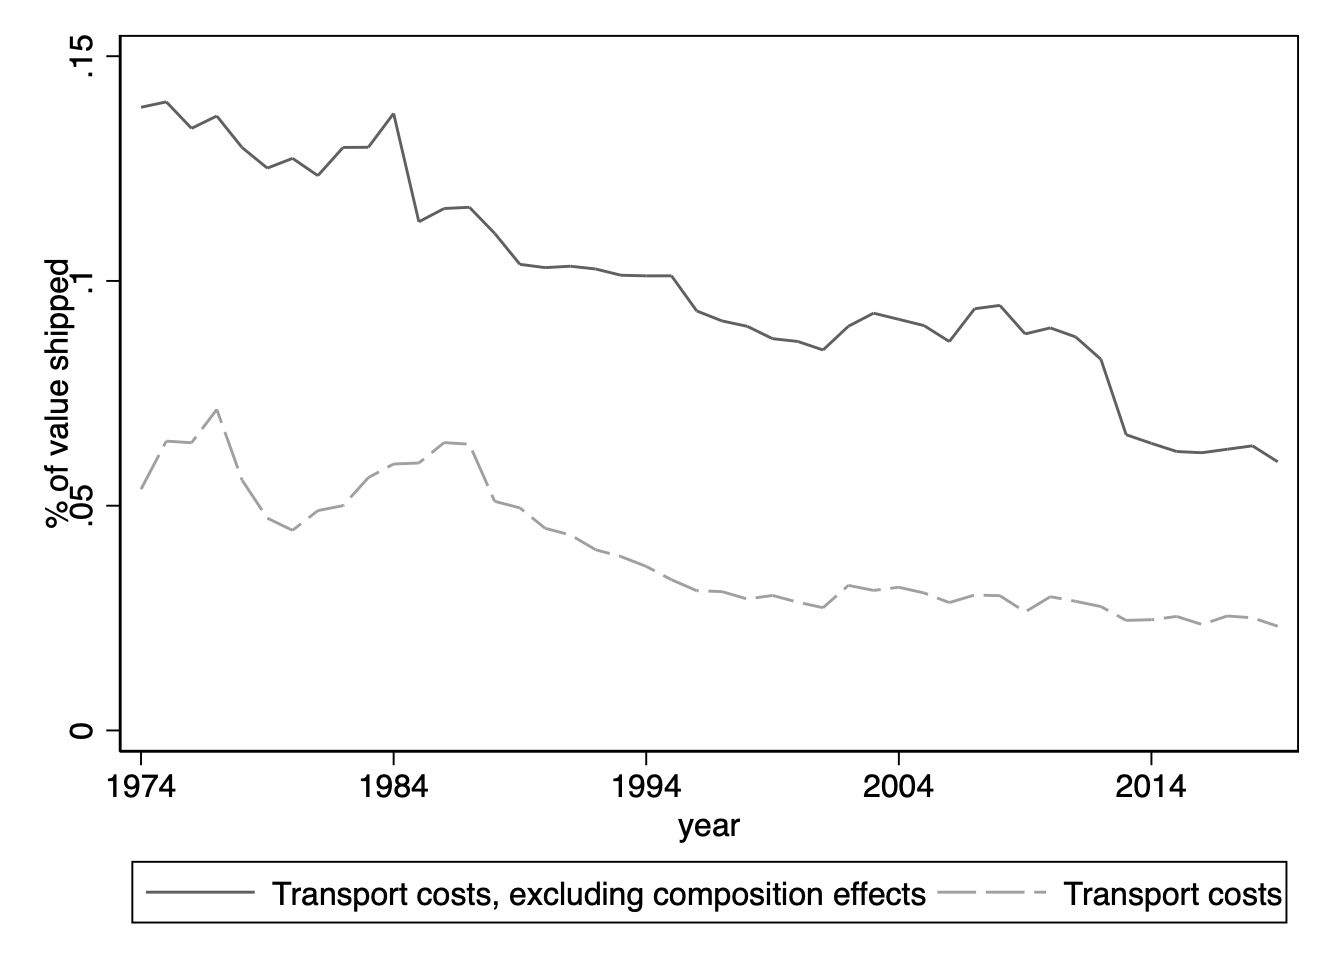
\includegraphics[width=2.5in, height=1.8in]{figure5_comme_hummels.jpg}
%& 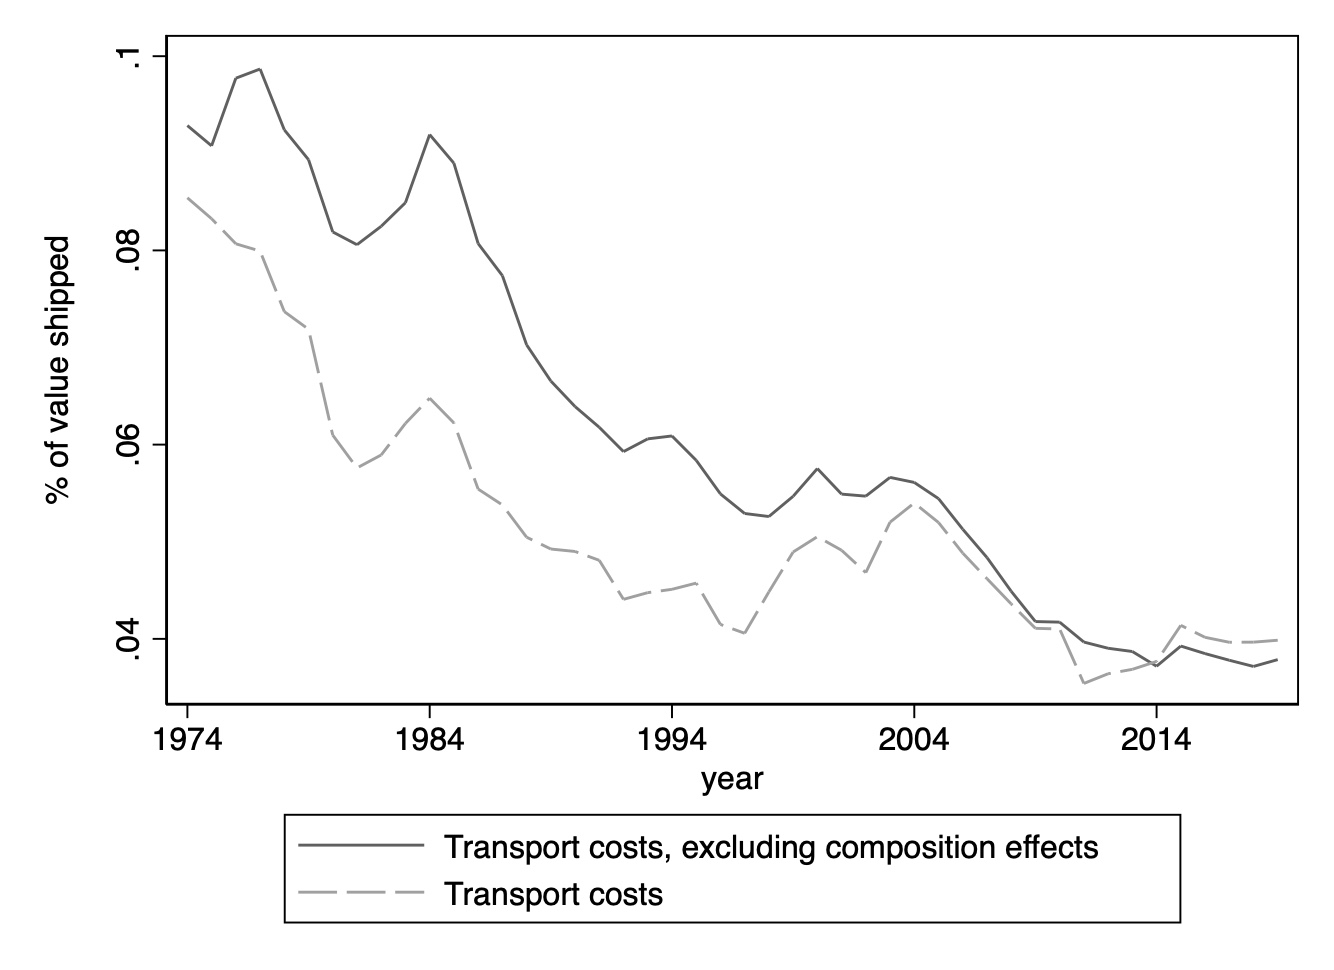
\includegraphics[width=2.5in,height=1.8in]{figure6_comme_hummels.jpg} \\
{\small (c) Air } & {\small (d) Vessel}\\
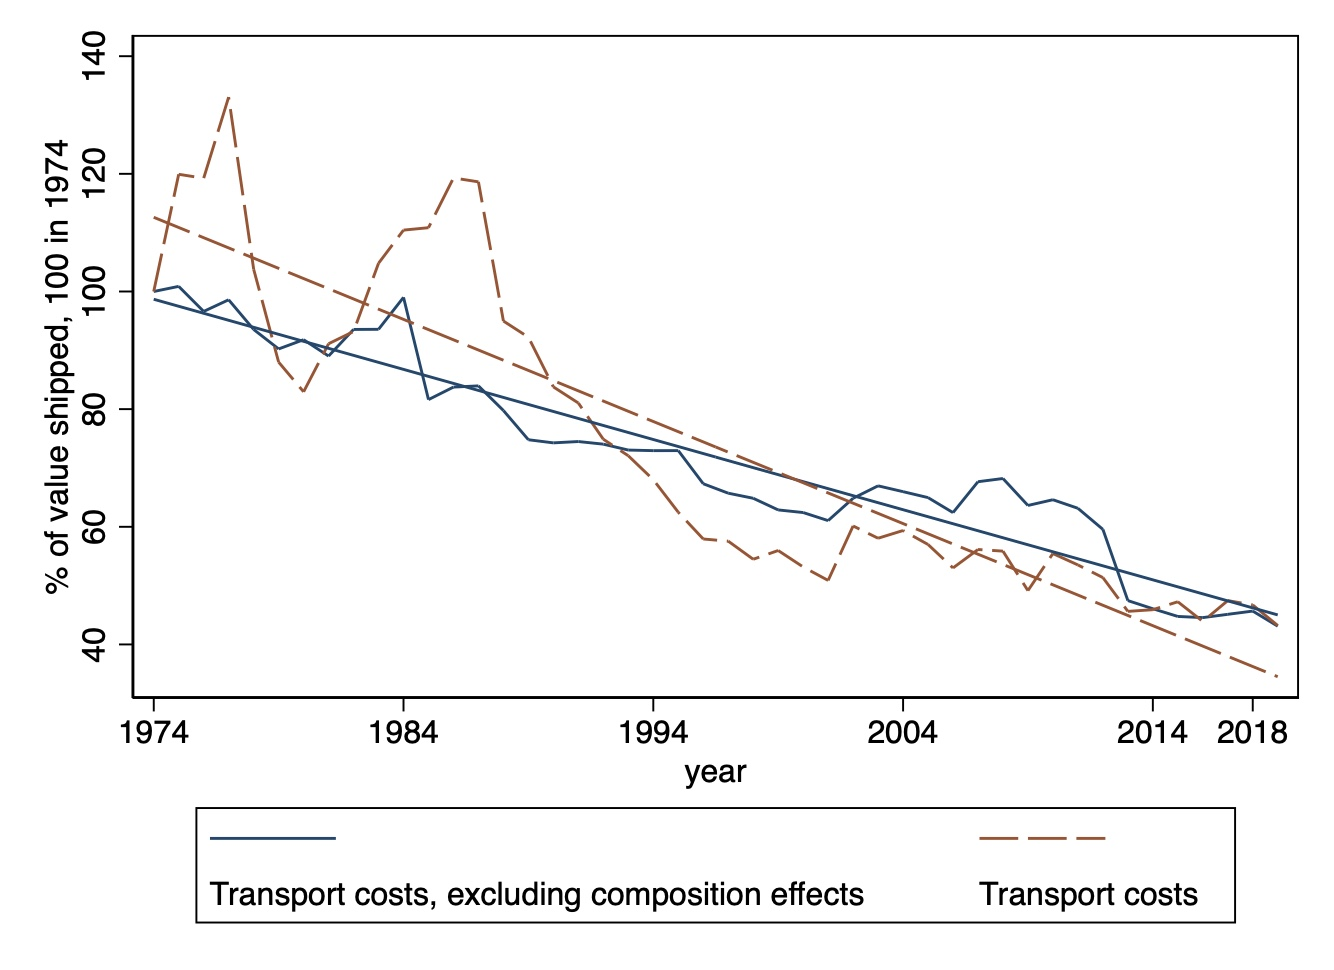
\includegraphics[width=2.5in, height=2in]{figure5_comme_hummels_base100.jpg}
& 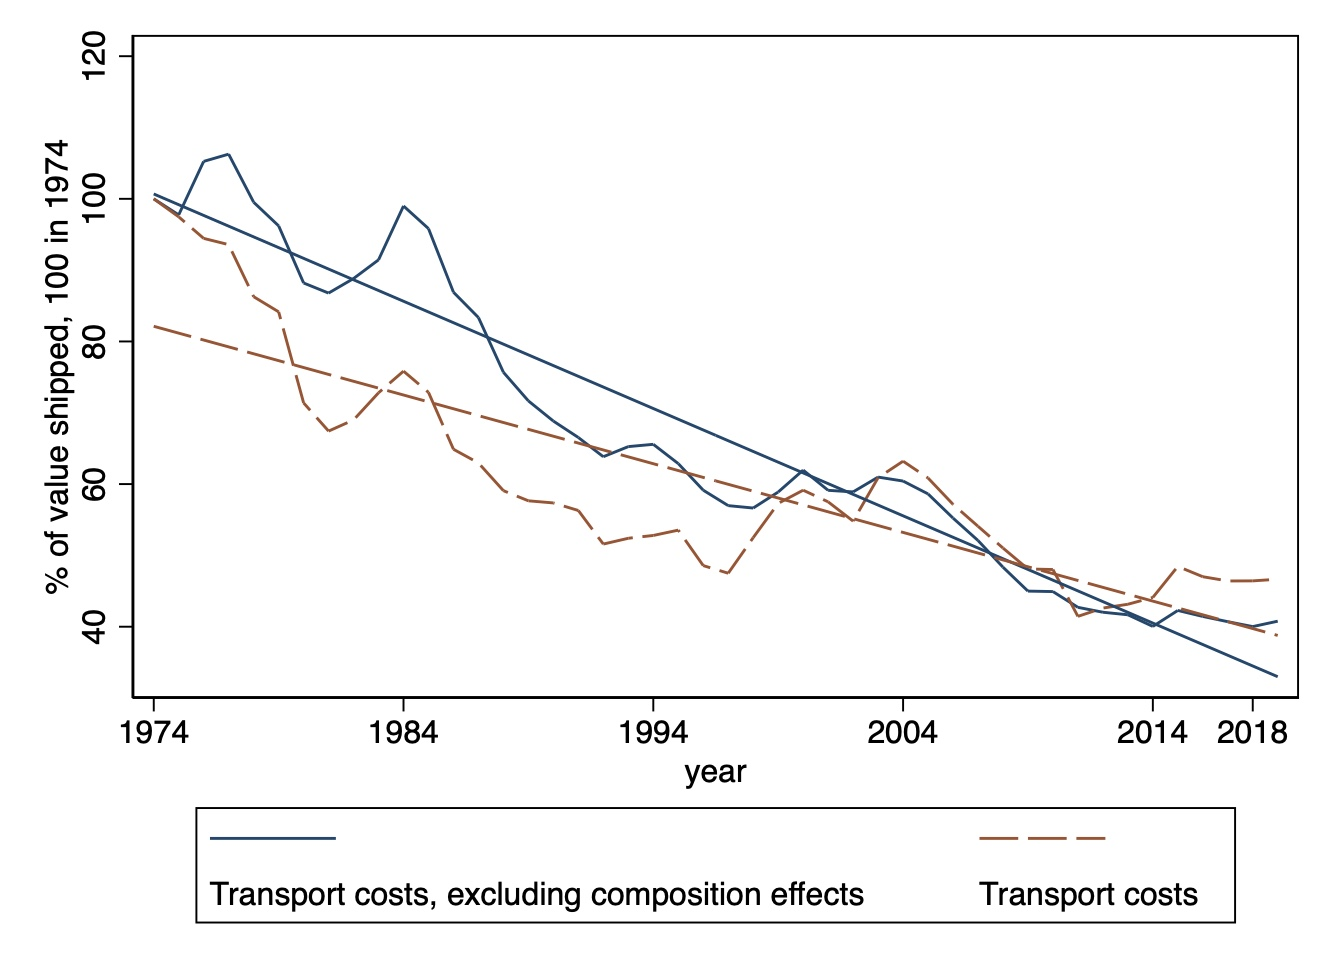
\includegraphics[width=2.5in,height=2in]{figure6_comme_hummels_base100.jpg} \\
\end{tabular}
	\begin{minipage}  [c]  {5in}
		\footnotesize
Total transport costs expressed in percentage of the value shipped, then built as indices with reference value 100 in 1974.
\end{minipage}
\end{center}
\end{figure}

These results stand in sharp contrast with the ones obtained with our methodology and reported in Figure \ref{fig:totalTC_compeffects_excl}.
Applying \cite{hummels2007} method, we find that the composition effects tend to partly offset the decrease in transport costs in both air and vessel shipping, as the downward trend is of higher magnitude for the fitted rate than the unfitted rate, especially for vessel (Panel (d)). Yet, this result is overturned when we allow for more flexibility in the role of the additive component, as indicated in Figure \ref{fig:totalTC_compeffects_excl}, Panels (c) and (f).\medskip

Assuming a varying share of the additive component over time, product and country partner indeed modifies the decomposition of the trend reduction of transport costs between the one attributable to trade composition effects and the reduction in the ``pure'' transport costs.
In both air and vessel transports, we thus find that this last dimension is the main driver of the reduction in international transport costs observed over time, in particular in air transport.
Complementing the findings of Section \ref{sec:results_decomposition}, these results highlight the importance of integrating the additive dimension of international transport costs, with the aim here of characterizing their time trends.

\section{The role of additive cost: Theoretical insights}\label{sec:theory}


In this section, we explore the implications of our empirical results on theoretical grounds. Over the last decade, several papers examined the implications of non-ad-valorem costs. \cite{Kropf-Saure-JIE-2016} estimate the size and shape of per-shipment costs based on Swiss data. \cite{Alessandria-et-al-AER-2010} and \cite{Hornok-et-al-RES-2015} point out the role of per-shipment costs in generating ``lumpiness'' in international trade transactions. \cite{Hornok-et-al-JIE-2015} focus on administrative costs incurring with every shipment, and draw welfare conclusions regarding the variations of these costs. We have complemented these studies by providing a long-run characterization of both the additive and the multiplicative component of transports costs. In this section, we use our empirical results to investigate the welfare consequences of the reduction in international transport costs observed over 1974-2019, contrasting two cases. One case assumes that the reduction was achieved solely through the decline of ad-valorem costs, as modeled in standard New Trade theoretical approaches. The other case builds on the results of our empirical investigation to assume that the reduction was achieved by a combined reduction in the ad-valorem and the additive components, as modeled by the addition of additive costs to the canonical \citet{melitz} model.\smallskip
%While the bulk of the trade literature investigates the role of trade costs modelled as ad-valorem costs (e.g., ad-valorem trade costs), not much is said about the role of the additive component. One potential explanation is the lack of empirical estimates about the size of additive costs. Our results may thus usefully palliate this limitation.

Our aim is related to \cite{Irrazabal_2015}, \cite{sorensen2014} and \cite{Lashkaripour_JIE2020}. We proceed in a different way though. \cite{sorensen2014} explores the welfare effects of a trade costs reduction depending on whether they are either fully ad-valorem or fully additive on analytical grounds. In contrast, as in \cite{Irrazabal_2015}, we provide a quantification of such welfare gains. As \cite{Irrazabal_2015} provide estimates of transport costs only for one year (2004), their assessment of the welfare effects of a trade cost increase is based on a ad-hoc assumption (specifically, of a 5\% increase in the ratio of additive cost to the median fas price). Unlike them, we can exploit our database time span to ground our study in the observed reduction of transport costs from 1974 to 2019. \cite{Lashkaripour_JIE2020} uses a partial-equilibrium model with perfect competition and builds on its result that for denumerable goods, per-unit additive transport costs are very small to find a very small welfare effect of additive costs. We look at the whole range of goods over a longer period and use a \citet{melitz} model like \cite{sorensen2014} and \cite{Irrazabal_2015}. In that context,
%\cite{Lashkaripour_JIE2020} obtains that welfare gains are not substantially different whether the transport cost decrease implies an additive component or not. This stands in contrast with the conclusion reached by \cite{sorensen2014} (analytically) and \cite{Irrazabal_2015} (quantitatively) in M\'{e}litz's type models.
we find (see below) the transport cost reduction implies substantially larger welfare gains when they are achieved through a reduction in the additive component.

%That said, it should be noted the case with additive costs in \cites{Lashkaripour_JIE2020}paper relies on a negligible share of additive costs. In this context, one might expect that whether additive costs are present or not makes little difference. As underlined by \cite{Lashkaripour_JIE2020}, a second explanation may rely on the modeling framework. While \cite{Lashkaripour_JIE2020} relies on a perfectly competitive environment,
Using a model with monopolistic competition and firm selection \`{a} la \cite{melitz} or \cite{chaney2008}, as did \cite{sorensen2014} and \cite{Irrazabal_2015} makes a difference. In this setting, we show that additive costs do modify the selection of firms on both the domestic and the export markets, e.g the extensive margin of trade, whose role in the welfare gains of trade cost reduction lies at the heart of the New Trade models  \`{a} la \cite{melitz}. Leaving aside the selection issue leads to an underestimation of the welfare gains that can be achieved by a reduction in additive transport costs.

\subsection{The model}


We rely on the model developed by \cite{sorensen2014}, which amends the two-country model of \cite{melitz} with monopolistic competition and endogenous firm entry to include additive costs.\footnote{\cite{Irrazabal_2015} adopt the multi-country model of \cite{chaney2008}.
%, consistently with their database that documents the exports of Norwegian firms in various destination markets worldwide.
We choose to retain the \cite{melitz} model, in its simplest form with one sector and two symmetric countries.
%, picking up the average estimated values of transport costs based on our unique importer country, e.g. the US.
Sticking to this canonical set-up allows us to illustrate the role of additive costs in a transparent and intuitive way.}
%Since our focus in on the role of additive versus ad-valorem transport costs, we directly present the two-country version of the model, with the two countries (Home and Foreign) being perfectly symmetric.
For the sake of space, we  present here only the building blocks of the model. More details can be found in Appendix \ref{app:theoretical_model}.

\subsubsection{Households}

In each country, the representative household exogenously supplies $L$ units of labour and maximizes utility $\mathcal{U} = \left[ \int_{\omega \in \Omega}c(\omega)^{\frac{\sigma-1}{\sigma}} d\omega \right]^{\frac{\sigma}{\sigma-1}}$, with $\sigma>1$ the elasticity of substitution between varieties $\omega$. She chooses her consumption $c(\omega)$  within the set $\Omega$ of available varieties (both domestic and foreign), subject to her budget constraint: $\int_{\omega \in \Omega} p(\omega) c(\omega) dw \leq E$, with $p(\omega)$ the consumer price of variety $\omega$ and $E$ nominal expenditures. The optimal demand function for variety $\omega$ is: $c(\omega) = \left(\frac{p(\omega)}{P}  \right)^{-\sigma} \frac{E}{P}$ with the associated optimal price index $P$ equal to $P = \left[ \int_{\omega \in \Omega}p(\omega)^{1-\sigma}d\omega\right]^{\frac{1}{1-\sigma}} $.


\subsubsection{Firms}

As in \cite{melitz}, firms are in monopolistic competition, each producing a differentiated variety using labor as sole production factor. Both countries are perfectly symmetric, the labor market equilibria impose an unique international wage that we use as the num\'{e}raire. At entry, each firm pays a sunk entry cost $f_e$ and subsequently draws its productivity level $\varphi$ from a known distribution $G(\varphi)$.  At each point in time, a firm can be terminated
%be hit by a death shock
at the exogenous probability $\delta>0$.
The production of $q$ units requires employing $l(q|\varphi) = f+\frac{q}{\varphi}$, units of labor, with $f$ the fixed cost of production. Exporting is subject to an extra fixed cost $f_x$ and variable exporting costs of two types: an ad-valorem cost that depends on the value traded $\tau\geq 1$ (as in \citealp{melitz}) and an additive cost depending on the quantity (weight) transported, $t\geq 0$. This $t$ is our innovation compared to the canonical Mélitz model.

Following \cite{melitz}, we solve the program of firms backwards. First, we solve for the maximizing profit behavior after entry. Second, we determine the entry conditions on both domestic and exporting markets.\medskip
\paragraph{Profit-maximizing behaviors} After entry, and conditional on being able to export, firms set a specific price on each destination market. The firm sets a constant markup on its marginal cost, which is a decreasing function of the firm's productivity $\varphi$, but also takes into account both components of trade costs on the destination market (see  Appendix \ref{app:theoretical_model}):
\begin{eqnarray}
p_d(\varphi) &=& \frac{\sigma}{\sigma-1}\frac{1}{\varphi} \notag \\
p_x(\varphi) &=& \frac{\sigma}{\sigma-1}\left[\frac{\tau}{\varphi} +t \right] \label{eq:px}
\end{eqnarray}

Under the assumption of symmetric countries (implying $E=E^\ast$ and $P=P^\ast$), one can compute the profits on the domestic and export markets ($\pi_d(\varphi)$ and $\pi_x(\varphi)$) respectively as:
\begin{eqnarray}
\pi_d(\varphi)  &=& \frac{r_d(\varphi)}{\sigma} - f = B \varphi^{\sigma-1} - f \label{eq:pid_rd}\\
\pi_x(\varphi) &=& \frac{r_x(\varphi)}{\sigma} - f_x = B \left[ \frac{\tau}{\varphi} + t\right]^{-(\sigma-1)} - f_x \label{eq:pix_rx}
\end{eqnarray}
\noindent $r_d(\varphi)$ and $r_x(\varphi)$ are the sales revenues on each market (see Appendix \ref{app:theoretical_model} for a detailed expression). $B \equiv \frac{1}{\sigma-1}\left(\frac{\sigma}{\sigma-1}\right)^{-\sigma}P^{\sigma-1}E$ . Profits increase with productivity $\varphi$.Only sufficiently productive firms are able to cover the fixed costs of operating in a given market. Further, in presence of trade costs, profits for a given productivity are lower on the export market than on the domestic market.
%a given firm of productivity $\varphi$ makes a lower export profit than on its domestic market, conditional on being productive enough to export.
We now determine the productivity threshold associated to the entry conditions.


\paragraph{Zero-cutoff profit conditions} Given the fixed costs on both the domestic and the export markets, only firms with a productivity above $\varphi^\ast$ will serve the domestic market, and only firms with a productivity above $\varphi_x^\ast$ will export. The two productivity thresholds can be linked according to:
\begin{equation}
\frac{\varphi_x^\ast}{\tau+t\varphi_x^\ast} = \varphi^\ast \left( \frac{f_x}{f} \right)^{\frac{1}{\sigma-1}} \label{eq:link_thresholds}
\end{equation}

Following \cite{melitz} and the subsequent literature, we impose selection on the export market, (i.e. $\varphi_x^\ast > \varphi^\ast$). From Equation (\ref{eq:link_thresholds}), this condition writes down as $\left[\tau+ t\varphi^\ast_x \right] \left( \frac{f_x}{f} \right)^{\frac{1}{\sigma-1}} >1$. In contrast to the ad-valorem only case, due to additive costs ($t>0$), the export selection condition depends on the equilibrium of the model (through $\varphi^\ast_x $) and cannot be imposed ex-ante by an appropriate restriction on parameters. We check this condition holds numerically when solving the model.
%\footnote{This is no longer the case under ad-valorem costs only. In this case, with $t=0$, we find the usual condition that $\varphi^\ast_x >\varphi^\ast$ iif $\tau^{\sigma-1}\frac{f_x}{f}>1$.}



\subsubsection{Aggregation, firm entry and exit}

\paragraph{Aggregation} The general equilibrium is characterized by a mass $M$ of producing firms in each country associated with a distribution $\mu(\varphi)$. Given the productivity threshold $\varphi^\ast$, $\mu(\varphi)$ is equal to:
%the conditional distribution of $g(\varphi)$ on the subset $\left[\varphi^\ast, \infty\right)$:
\begin{eqnarray}
\mu(\varphi) &=& \left\{
\begin{array}{ll}
\frac{g(\varphi)}{1-G(\varphi^\ast)}, & \text{if } \varphi\geq \varphi^\ast  \\
0 & \text{otherwise}
\end{array}
\right.  \label{eq:muofphi}
\end{eqnarray}
\noindent with $1-G(\varphi^\ast)$ the probability of successful entry on the domestic market. Conditional on being active on the domestic market, a subset mass $M_x$ of firms export abroad. $\mu_x(\varphi)$ can be similarly defined as the conditional distribution of productivity on the export market, e.g. on the support $\left[ \varphi^\ast_x,\infty\right)$.
Further defining $M_T = M+M_x$ as the total mass of varieties accessible to the consumers, $\widetilde{\varphi}_T$ the weighted average of firms productivities on the domestic market, one can show that the welfare per worker can be written as (see Appendix \ref{app:theoretical_model}), with $\rho =  \frac{\sigma-1}{\sigma}$ inversely related to the markup rate:
\begin{equation}
\mathcal{W} = \rho \widetilde{\varphi}_T M_T^{\frac{1}{\sigma-1}} \label{eq:Welfare}
\end{equation}

\paragraph{Free-entry condition} Assuming free entry, the expected net present value of entry is driven to zero.
Defining $\bar{\pi}$ as the average profit conditional to entry, this free-entry condition rewrites as:
\begin{equation}
\left(1-G(\varphi^\ast)\right)\frac{\bar{\pi}}{\delta} = f_e \label{eq:FEC}
\end{equation}
As shown in Appendix \ref{app:theoretical_model}, the free-entry market condition can be rewritten as:
\begin{equation}
\bar{\pi} = \left\{\left(\frac{\widetilde{\varphi}^\ast}{\varphi^\ast}\right)^{\sigma-1}-1 \right\}f +  \frac{1-G(\varphi_x^\ast)}{1-G(\varphi^\ast)}\left\{\left[\left(\frac{\widetilde{\varphi}_x^\ast}{\varphi_x^\ast}\right)\left(\frac{\tau+ t \varphi^\ast_x}{\tau+ t \widetilde{\varphi}^\ast_x}\right)\right]^{\sigma-1}-1 \right\}f_x \label{eq:ZCP}
\end{equation}
\noindent with $\widetilde{\varphi}^\ast$ and $\widetilde{\varphi}_x^\ast$ the weighted average productivities of domestic and exporting firms respectively (see Equations (\ref{eq:def_phitilde}) and (\ref{eq:def_phitildex}) in Appendix \ref{app:theoretical_model}).


\subsection{Calibration}

Following a standard assumption in this literature (\cite{Irrazabal_2015}, \cite{melitz-redding-Handbk-IT-2014}), the distribution in firm productivity is assumed to follow a Pareto distribution with parameters $(\varphi_{min},k)$. This allows a full analytical solving of the M\'{e}litz model. This is no longer the case in the presence of additive costs (see Appendix \ref{app:theoretical_model}). In this case, we need to rely on the model's simulations to determine the steady state. This drives us to calibrate the structural parameters of the model. To do so, we usevalues commonly retained in the literature, as reported in Table \ref{tab:calib_horsTC}.

\begin{table}[htb]
  \centering
  \caption{Calibration (1)} \label{tab:calib_horsTC}
\begin{center}
	\begin{tabular}{lll}
& Value & Reference\\
\hline
$\sigma$ & 4 & \cite{Irrazabal_2015}\\
$f_e$ & 1 & \cite{ghironi}\\
$f$ & 0.033 & \cite{ghironi} \\
$L$ & 1 & Arbitrary\\
$\delta$ & 0.1 & \cite{ghironi}, \cite{Irrazabal_2015}\\
$k$ & 4 \\
$\varphi_{\text{min}}$ & 1 & \cite{ghironi}, \cite{Irrazabal_2015}\\ \hline
\multicolumn{3}{l}{Fixed export cost } \\
$f_x $ & 0.08 & Share of exporting plants = 21\% (\cite{ghironi}, based on BEJK, 2003) \\
& 0.06& Share of exporting plants = 39\% (\cite{Lincoln_McCallum2018}) \\
\hline
\end{tabular} 
\end{center}
{\parbox[l]{10cm}{ \vspace{4pt}\footnotesize{Notes: $f$ is endogenously revealed such that all firms produce in autarky. $f_x$ can take two values, depending on the share of exporters considered that might differ between the initial steady state (21\%, based on early 1980s value) and the final steady state (39\%, based on 2006 value), according to the references provided above.}}}
\end{table}

The one exception is the value for the two additive and ad-valorem transport costs, for which we use our empirical estimates of Section \ref{sec:results_decomposition} for the years 1974 and 2019, as reported in Table \ref{tab:calib_TC}.

\begin{table}[htb]
  \centering
  \caption{Calibration (2)}\label{tab:calib_TC}
\begin{center}
	\begin{tabular}{l|cc|cc|cc|cc}
& \multicolumn{4}{|c|}{Air transport} & \multicolumn{4}{|c}{Maritime transport} \\ \hline
& \multicolumn{2}{|c|}{1974} & \multicolumn{2}{c}{1974} \\
& (1) & (2) &  (3) & (4) & (5) & (6) &  (7) & (8)\\ \hline
Total TC (\% of fas price) & 6.2 & 6.2 & 2.8 & 2.8 & 10.5 & 10.5 & 4.1 & 4.1 \\
$\tau$ (in \%) & 6.2 & 3.6 & 2.8 & 2.2 & 10.5 & 5.4 & 4.1 & 2.3\\
$t/\widetilde{p}_x$ (in \%) & 0 & 2.6 & 0 & 0.6 & 0 & 5.1 & 0 & 1.8\\
\hline \hline
\end{tabular} 
\end{center}
{\parbox[l]{14cm}{ \vspace{4pt}\footnotesize{Notes: In Columns (1), (3), (5) and (7), we model ad-valorem costs only. In Columns (2), (4), (6) and (8), we model both ad-valorem and additive costs. $t$ is calibrated so that the ratio $t/\widetilde{p}^{\text{fas}}_x$ from the model matches its empirical target, with $\widetilde{p}^{\text{fas}}_x$ the average fas price set in place by those domestic firms that export. We theoretically define the export fas price through: $p_x = \tau \widetilde{p}_x^{\text{fas}} +t$. TC = Transport Costs. The empirical targets for 1974 and 2019 are based on the estimated linear trend over the period.}}}
\end{table}


We are interested in studying the normative consequences of trade liberalization in presence or not of additive costs. To that aim, we will compare the equilibrium based on the values of transport costs at the beginning (1974) and at the very end of our estimation period (2019), in two settings: the first one including only ad-valorem transport costs (uneven columns in Table \ref{tab:calib_TC}). We here apply the estimated reduction in total variable transport costs ``as if'' it was solely attributable to the ad-valorem component. The second scenario includes both additive and ad-valorem costs (even columns in Table \ref{tab:calib_TC}). In this case, we rely on the estimates of transport costs involving both additive and ad-valorem components. The reduction in international transport costs channels through both its additive and ad-valorem components. Besides, \cite{Lincoln_McCallum2018} document the large increase in the number of exporting firms in the US between the mid 1980s et the mid 2000s, with a share of exporting firms raising by 52\% over this period. This can be captured in the model through a reduction in the fixed export cost $f_x$ (as reported in Table \ref{tab:calib_horsTC}). Accordingly, we will assess the effects of the trade liberalization assuming a joined reduction in both the variable transport costs ($\tau, t$, based on our empirical estimates) and the fixed export cost $f_x$.
%\footnote{We endogenously determine the initial value of $f_x$ such that the initial steady state (with 1974 values of transport costs) implies a share of exporting firms equal to 21\%, as in  \cite{ghironi} based on the value estimated by \cite{BEJK-AER-03} in the early 1990s. In the final steady state, $f_x$ will be revealed such that this share of exporting plants has increased by 85\% (i.e., from 21\% to 39\%), based on the evidence reported in \cite{Lincoln_McCallum2018}, along with the 2019 values of variable transport costs xxxx GD redondant avec la note du tableau, non ?xxxx }



\subsection{Trade cost reduction: The importance of additive costs}

Our empirical results point to two important conclusions: First, additive costs represent a non-negligible part of overall international transport costs. Second, total transport costs have strongly reduced over 1974-2019, and the decrease is particularly marked in the additive component in air transport. We exploit the theoretical implications of these empirical findings by running a comparative statics analysis following a reduction in variable transport costs based on our estimates in 1974 and 2019, by transport mode.
%Specifically, we contrast two cases: In the first scenario, we assume that only ad-valorem costs apply. We hence apply the estimated reduction in total variable transport costs ``as if'' it was solely attributable to the ad-valorem component. In the second scenario, we rely on the estimates of transport costs involving both additive and ad-valorem components. The consequences of the reduction in international transport costs through both its additive and ad-valorem components.

In running this exercise, we also take into account the fact that the share of exporting firms has substantially increased since the 21\% value reported in \cite{BEJK-AER-03} (and consistent with the value estimated by \citet{Lincoln_McCallum2018} for 1987 on US data). According to \cite{Lincoln_McCallum2018}, this share roughly amounts to 39\% in the mid 2000s. This can be matched in the model by resetting the (lower) value of the export fixed cost $f_x$ accordingly. Our preferred scenario thus embeds the two dimensions of trade cost reduction: the reduction of transport costs along with the reduction of the export fixed cost.



The results are reported in Table \ref{tab:resultats_modele}, panel (2), by transport mode (for Air (Columns (A)-(B)) and Vessel (Columns (C)-(D) respectively.\footnote{For sake of space saving, we only report the welfare consequences of trade liberalization, depending on the structure of transport costs, even if we refer to the positive effects (in terms of number of firms, threshold and average productivities, etc.) to explain the underlying mechanisms. The whole set of results is available upon request to the authors.} Specifically, we report the change in total transport costs (expressed in percentage points, and based on the raw numbers reported in Table \ref{tab:calib_TC}), decomposed in its two dimensions (additive and ad-valorem); as well as the welfare change, both in absolute and in relative terms.
We also simulate an alternative scenario where only the variable transport costs decrease, the fixed export cost being constant at its initial value. This has two purposes. It allows us to better highlight the specific mechanisms involved by a reduction in additive costs versus a reduction in ad-valorem costs. It also delivers a relevant robustness check on the welfare implications of additive costs. These results are reported in Table \ref{tab:resultats_modele}, panel (1).\footnote{Under a constant fixed export cost, we also compare two alternative cases. Starting from the values observed in 1974, we simulate \textit{(i)} the observed reduction in the additive cost $t/\widetilde{p}^{fas}$, maintaining the ad-valorem component at its initial (1974) value, and  \textit{(ii)} the opposite case, the observed reduction of ad-valorem costs ($\tau$), maintaining the additive component at its initial value. The quantitative results strongly confirm that, keeping cost level constant, additive costs are more detrimental for welfare than ad-valorem costs.
%, and the larger welfare gains when this specific component of international trade costs is reduced.
See Appendix \ref{app:theoretical_model}, Table \ref{tab:results_model_appendix} for the results}.


\begin{table}[htbp]
  \centering
  \caption{Trade cost reduction: The role of additive costs} \label{tab:resultats_modele}
\begin{center}
\begin{tabular}{l||c|c||c|c}
\hline
Mode & \multicolumn{2}{|c||}{Air} & \multicolumn{2}{c}{Vessel} \\ \hline
& (A) & (B) & (C) & (D)  \\
Reduction in: & $\tau$ only & $\tau$ and $t$ &$\tau$ only & $\tau$ and $t$\\  \hline
%$TC_{1974}$ & 0.062 & 0.062 & 0.062 & 0.062 & 0.105 & 0.105 & 0.105 & 0.105\\
%$TC_{2019}$ &  0.028 & 0.028 & 0.028 & 0.028&  0.041 & 0.041 & 0.041 & 0.041\\
$\Delta TC$ (in pp) &-3.8 &-3.8 &-4.9 &-4.9   \\
$\Delta \tau$ (in pp) & -3.8	&-1.95&-4.9&	-3.53	 \\
$\Delta t/\widetilde{p}_x^{\text{fas}}$ (in pp) & 0&	-1.8&	0&	-1.4\\ \hline
\multicolumn{4}{l}{(1) Constant fixed export cost} \\ \hline
$\Delta \beta$ (in pp) &0&-15.4&0&9.3 \\
$\Delta \mathcal{W}/\mathcal{W}$ (in \%) & 1.38&	2.46 & 1.71	&2.20 	 \\
\hspace{1em} Variety effect (\%)& -0.93 	&-2.57	&-1.09	& -1.88 \\
\hspace{1em} Price effect (\%)&2.34 &5.24	&2.85	& 4.19  \\
\hline
\multicolumn{4}{l}{(2) Lower fixed export cost} \\ \hline
$\Delta \beta$ (in pp) &0&-15.15&0&9.16 \\
$\Delta \mathcal{W}/\mathcal{W}$ (in \%) & 	\textbf{2.62}	&\textbf{3.66}	&	\textbf{2.83}&	\textbf{3.23 }  \\
\hspace{1em} Variety effect (\%)&1.19 &-0.45	&0.92	&0.23 \\
\hspace{1em} Price effect (\%)&	1.42 &	4.14&		 1.90&	3.0 \\ \hline \hline
\end{tabular}
\end{center}
{\parbox[l]{10cm}{ \vspace{4pt}\footnotesize{Notes: TC = Transport Costs, expressed in percentage of the average export fas price. The reduction in transport costs is expressed in percentage points. In Columns (B) and (D), we first simulate the observed reduction in $\tau$ and iterate on the reduced value of $t$ such that the simulated value of $t/\widetilde{p}_x^{\text{fas}}$ matches the empirical target.  }}}
\end{table}



In line with the literature, we find that a reduction of trade costs  induces welfare gains
% whatever the transport mode (and the associated magnitude of the transport costs decrease).
The originality of our results rather dwells on comparing the welfare gains depending on the type of cost reduction.
Welfare gains are higher when the trade cost reduction includes a decrease in additive trade costs.
This is consistent with the analytical results of \cite{sorensen2014} and the quantitative ones of \cite{Irrazabal_2015}.
%in a different exercise of trade liberalization though. \footnote{\cite{sorensen2014} compares the welfare effect of a trade costs reduction depending whether it is exclusively ad-valorem or exclusively additive, the comparison between both trade cost decreases being a criterion of equal impact on trade openness. Our quantitative model offers a more general and flexible set-up, as we can virtually consider all cases of trade liberalization. Based on our empirical estimates, we compare the effects of the same decrease in overall transport costs depending on 1) whether additive costs are present or not, and 2) when they are present, assuming that the trade cost decrease is achieved by a reduction of both additive and ad-valorem components.}
Quantitatively, the welfare gains are sizeable. In our preferred scenario, the reduction in variable transport costs in Air transport generates a relative welfare gain 40\% higher when such a reduction partly occurs through the additive component, rather than when it realizes through a decrease in iceberg costs only (Table \ref{tab:resultats_modele}, panel (2), Column (B) vs (A)). In maritime transport, the extra welfare gains due to the joined reduction of both transport costs components are more modest, with a magnitude of order of 14\%. This can be set in connection with the fact that in maritime transport, ad-valorem costs have reduced more than the additive ones, implying a larger $\beta$ at the end of the period.\footnote{See Appendix \ref{app:theoretical_model} for a similar result.}
%Closely related to our work, \cite{Irrazabal_2015} also quantify the welfare losses of imposing trade taxes depending on whether they are additive or ad-valorem. If we share a similar conclusion regarding the importance of additive costs, our empirical analysis allows us to simulate the effects of the reduction in transport costs actually observed in the data over the period 1974-2019, in all their dimensions (additive and ad-valorem).
\smallskip

What are the mechanisms? Recalling that welfare is the inverse of the price index, the explanation can be understood decomposing the welfare change in its two components, the variety effect and the price competitiveness effect. Considering Equation (\ref{eq:Welfare}), it is straightforward to get the welfare change as:
\begin{equation}
\frac{d\mathcal{W}}{\mathcal{W}_0} = \underbrace{\frac{1}{\sigma-1} \frac{d M_T}{M_{T0}}}_{\text{Variety effect}} +  \underbrace{\frac{d\widetilde{\varphi}_T}{\widetilde{\varphi}_{T0}}}_{\text{Price effect}} \label{eq:decompWelfare}
\end{equation}

We report the decomposition of the welfare gains in their two components in Table \ref{tab:resultats_modele}, under a constant fixed export cost (Panel (1)) and under our preferred scenario (Panel (2)). \medskip
%Closely related to our work, \cite{Irrazabal_2015} also quantify the welfare losses of imposing trade taxes depending on whether they are additive or ad-valorem. If we share a similar conclusion regarding the importance of additive costs, our empirical analysis allows us to simulate the effects of the reduction in transport costs actually observed in the data over the period 1974-2019, in all their dimensions (additive and ad-valorem).


\paragraph{Holding fixed costs constant} To understand the changes induced by the additive costs, we start by considering the scenario with a constant fixed export cost (Table  \ref{tab:resultats_modele}, Panel (1)). In this case, the welfare changes are solely attributable to the reduction in the variable transport costs, and the difference of results stems from the fact that the transport cost decrease involves an additive part or not.

Consider first the benchmark model \textit{\`{a} la M\'{e}litz} with only ad-valorem costs (Table \ref{tab:resultats_modele}, Panel (1), Columns (A) and (C)). The reduction in the iceberg cost induces a negative variety effect, which is yet
more than counteracted by a positive competitive effect. This is accounted for as follows. With the reduction in $\tau$, more firms can now export, but this also increases the expected average profit. This raises the productivity threshold to enter the domestic
market. Accordingly, the number of domestic active firms reduces, even if a larger number
of them is able to export. As a whole, the total number of varieties accessible to the
consumer reduces, which reduces welfare everything else equal.
This detrimental effect is counteracted by a positive price competitiveness effect. Due
to the tougher selection on the domestic market, the less productive firms no longer enter.
As a result, the average productivity on the domestic market increases, which pushes
the average productivity upwards. As reported in Table \ref{tab:resultats_modele}, the strength of the price
competitiveness effect dominates, inducing positive welfare gains with the reduction in
iceberg costs, consistently with the analytical results of \cite{melitz}.

What does it change when the reduction in international transport costs also occurs
through a reduction in its additive component? As reported in Table \ref{tab:resultats_modele}, panel (1), columns (B) and (D), the welfare gains are stronger than in the pure ad-valorem case. Again, the effect is quantitatively sizeable: Welfare gains are thus between 30\% and 78\% higher, depending on the transport mode. This is driven by a more positive price competitiveness effect and despite the more negative variety effect (comparing with Columns (A) and (C), same panel). This can be accounted for as follows.

As underlined by \cite{sorensen2014}, a reduction in the additive cost reduces the export-market price of the high-productive
exporters relative to the low-productive ones (as can be inferred from Equation (\ref{eq:px})).
Within the exporters category, this favors the more productive firms, whose market share,
e.g. revenues, increases relatively more (see Equation (\ref{eq:rx})). Everything else equal, this
pushes the average productivity on the export market upwards. Unlike the ad-valorem
costs, the reduction in additive costs induces a \textit{within-exporters selection effect}, in favor of
the more productive firms. At the general equilibrium, this \textit{within-exporters} selection effect
also affects the \textit{classic} selection effect at the extensive margin at the heart of the M\'{e}litz
(2003) model. As the expected export profit increases, it is necessary to be more productive
to satisfy the free-entry condition. Everything else equal, the threshold productivity
on the domestic market rises, as well as the average productivity. Accordingly, the
price competitiveness effect increases by more when the trade liberalization involves a reduction
in the additive component.

The welfare-dampening impact of the variety effect is also stronger under this scenario. Since the reduction in additive costs favors the more productive firms in terms of market share, entry on the export market is tougher leading to a much more modest increase in the
share of exporters. As the selection on the domestic market is also more stringent, the
mass of total active firms reduces by a larger amount. From the consumer side, this induces
a more negative variety effect that is welfare-detrimental everything else equal. As for the
pure-iceberg case though, the strength of the (larger) competitiveness effect dominates,
inducing positive welfare gains, and even larger when the trade liberalization involves a
reduction in additive costs.\medskip

\paragraph{Taking into account the reduction in fixed costs} As mentioned above, our preferred scenario includes, in addition to the reduction of variable costs, a reduction in fixed export costs, based on \cite{Lincoln_McCallum2018}'s empirical evidence.
The associated welfare gains are reported in Table \ref{tab:resultats_modele}, Panel (2).
Two results emerge.
First, the welfare gains induced by the trade cost reduction are stronger in magnitude.
While this is not a surprising result \textit{per se} (we now consider two sources of international frictions, rather than one), this exercise yet delivers a quantification of the welfare gains associated with a reduction in the fixed export cost: They are substantial, higher by around 50\% relative to the case when only the two components of the variable transport costs decrease.\footnote{Under the scenario with only ad-valorem costs (Columns (A) and (C)), the extra welfare gains due to the reduction of $f_x$ are much higher, by 66\% (Vessel) and 89\% (Air) respectively. Put differently, the reduction of the sunk export cost accounts for the majority of welfare gains. This is not the case under additive variable costs; in this case, the reduction of the distortion due to the additive costs continues to substantially matter in the welfare-enhancing effect of the globalization process.}  This can be accounted for as follows. The reduction in the fixed export cost pushes more firms to export everything else equal. This increases the number of available imported varieties for the consumer, which counteracts the reduction in the number of domestic varieties induced by the tougher selection on the domestic market. As a result, the joined reduction in variable costs and in $f_x$ dampens the negativity of the variety effect (which even turns out to be positive in some cases). This, combined with a positive price competitiveness effect, accounts for the stronger welfare gains reported in Panel (2).

Second, the main message of the paper remains valid. The welfare gains of the trade cost reduction are still higher when part of this structural change is achieved through a reduction in additive transport costs. Quantitatively, the effect remains sizeable: Welfare gains are between 14\% and 40\% higher when the globalization process involves a reduction in additive costs. Put differently, the reduction in the fixed export cost does not seem to depend on the composition of the variable costs. In the end, the welfare gains are the highest when trade costs reduction induces a combined reduction in both variable and fixed export costs, and when (part of) the reduction in the variable part is achieved through a decrease in the additive component, as observed empirically.\smallskip

In line with \cite{sorensen2014} and \cite{Irrazabal_2015}, our overall theoretical results point out the importance of taking into the additive components of international trade costs. Additive costs have a substantial impact on the extensive margin of trade, by affecting the composition of the basket of exported goods. This, in turn, has important consequences in normative terms. Relying on our empirical estimates of transport costs over 1974-2019, we obtain that the 60\% reduction of variable costs in Air transport, combined with the reduction in the fixed export costs, has induced an 3.66\% increase in welfare, much higher than if only iceberg costs were modeled (2.6\%). A similar result applies with the observed 57\% reduction in total variable costs in maritime transport along with the reduction in the fixed export costs, with a relative increase in welfare by 3.2\% (as compared to 2.8\% in a pure ad-valorem world). Neglecting the existence and long-term evolution additive costs thus leads to a substantial underestimation of the welfare gains of trade cost reduction.


\section{Conclusion \label{sec:conclu}}

This paper assesses the magnitude and the role of additive international transport costs. Empirically, we exploit the differences between the import and the export prices taken from the US import database over 1974-2019, to estimate the two components (additive and ad-valorem) of transport costs, by transport mode (air or ocean). We find that additive costs are quantitatively sizable: On average over the period, they amount to 2.8\% of the export price unit values for ocean shipping, and 1.7\% for air transport, accounting for 30\% and 45\% of total transport costs in air and maritime transport respectively.

To what extent should we care about additive costs? Our paper addresses this question through two different angles. First, we show the importance of integrating the additive component in accounting for the time trend of international transport costs observed over 1974-2019. Allowing for a varying share of additive costs in the product/country/time dimension, we find that the decrease of international transport costs observed in the data is mostly attributable to a reduction in the \textit{pure} transport costs, with trade pattern composition effects playing a small role. If anything, trade composition effects have contributed to amplifying the reduction in the pure transport costs in maritime transport.

Second, we revisit the question of the welfare gains from trade liberalisation to shed light on the role of additive costs on this issue. To this aim, we amend the canonical M\'{e}litz (2003) model with additive costs. Relying on our empirical estimates of transport
costs over 1974-2019, our preferred scenario shows an extra welfare gain higher by 14\% and 40\% respectively in vessel and air transport when the transport cost decrease encompasses a reduction in its additive
component (as we document empirically) relative to a pure ad-valorem reduction. In both aspects, our results highlight the importance of the additive component in accounting for international transport costs.

Our results could be extended in two main ways.
On the empirical side, one may want to go deeper into the structural determinants of (pure) transport costs - i.e.
identify the respective roles of handling costs, insurance and freight at the root of the gap between export and import prices.
On the theoretical side, our results call for exploring the role of additive costs in shaping international trade flows in richer New Trade models than the canonical M\'{e}litz model used so far, and in affecting the international transmission of business cycles.
This is left for further research.



\newpage
\bibliographystyle{apalike2}
\bibliography{biblio}


\newpage


\appendix

\clearpage

%\appendix
\setcounter{table}{0}
\renewcommand{\thefigure}{A.\arabic{figure}}
\renewcommand{\thetable}{A.\arabic{table}}


\section{Data Appendix \label{app:data}}


The Customs value is the value of imports as appraised by the U.S.
Customs and Border Protection in accordance with the legal requirements of the Tariff Act of 1930, as amended.
This value is generally defined as the price actually paid or payable for merchandise when sold for exportation to the United States, excluding U.S.
import duties, freight, insurance, and other charges incurred in bringing the merchandise to the United States.
The term ``price actually paid or payable'' means the total payment (whether direct or indirect, and exclusive of any costs, charges, or expenses incurred for transportation, insurance, and related services incident to the international shipment of the merchandise from the country of exportation to the place of importation in the United States) made, or to be made, for imported merchandise by the buyer to, or for the benefit, of the seller.
In this respect, the ``custom value'' corresponds to the fas price (``free-alongside'' price) delivered by the seller. Let us clarify here the difference with the fob price. The fas price means that the seller must transport the goods all the way to the dock, close enough to be reached by the crane of the ship it will be transported in. It is also the seller's responsibility to clear the goods for export. The fob price means that the seller is obligated to bring the goods all the way to the port, clear the goods for export, and see that they are loaded onto the ship nominated by the buyer. Once the goods clear the railing of the vessel, the buyer assumes the risk. Note that this term is used exclusively for maritime and inland waterway transport. More information is available at: \url{http://www.census.gov/foreign-trade/reference/products/catalog/fl_imp.txt}. \smallskip



The import charges represent the aggregate cost of all freight, insurance, and other charges (excluding U.S.
import duties) incurred in bringing the merchandise from alongside the carrier at the port of exportation in the country of exportation and placing it alongside the carrier at the first port of entry in the United States.
In the case of overland shipments originating in Canada or Mexico, such costs include freight, insurance, and all other charges, costs and expenses incurred in bringing the merchandise from the point of origin (where the merchandise begins its journey to the United States in Canada or Mexico) to the first port of entry.

The cif (cost, insurance, and freight) value represents the landed value of the merchandise at the first port of arrival in the United States.
It is computed by adding ``Import Charges'' to the ``Customs Value'' (see definitions above) and therefore excludes U.S.
import duties.

\clearpage
\setcounter{table}{0}
\setcounter{figure}{0}
\renewcommand{\thefigure}{B.\arabic{figure}}
\renewcommand{\thetable}{B.\arabic{table}}

\section{Estimation at the 3-digit classification level \label{app:more_results}}

\subsection{Transport costs estimates: More detailed results}

In this section, we report more detailed results for the estimates for international transport costs, by transport mode on a yearly basis, when either additive costs are included in the estimation (Equation (\ref{eq:model_IetA})) or not (Equation (\ref{eq:model_nlI})), under our benchmark sectoral classification level (3 digit).
Specifically, we complement the results displayed in Table \ref{tab:summary_results} by reporting the estimates of international transport costs for a sample of years over 1974-2019, when the degree of classification retained ($s$) is at the 3-digit classification level (products are at 5-digit level).
Table \ref{tab:result_air_3d_detail} reports the results for air transport.
The results for vessel transport are displayed in Table \ref{tab:result_ves_3d_detail}.


\begin{table}[htbp]
	\centering
	\footnotesize{
	\caption{Air: Transport costs estimates, 3-digit level (selected years)}\vspace{5mm}
	\label{tab:result_air_3d_detail}%
	\begin{tabular}{lllllll}
\cline{1-7}
\multicolumn{1}{c}{} &
  \multicolumn{1}{|r}{1974} &
  \multicolumn{1}{r}{1980} &
  \multicolumn{1}{r}{1990} &
  \multicolumn{1}{r}{2000} &
  \multicolumn{1}{r}{2010} &
  \multicolumn{1}{r}{2019} \\
\cline{1-7}
\multicolumn{1}{l}{\textbf{Data}} &
  \multicolumn{1}{|r}{} &
  \multicolumn{1}{r}{} &
  \multicolumn{1}{r}{} &
  \multicolumn{1}{r}{} &
  \multicolumn{1}{r}{} &
  \multicolumn{1}{r}{} \\
\multicolumn{1}{l}{\hspace{1em}{$\#$ obs.}} &
  \multicolumn{1}{|r}{14,955} &
  \multicolumn{1}{r}{16,118} &
  \multicolumn{1}{r}{24,958} &
  \multicolumn{1}{r}{35,027} &
  \multicolumn{1}{r}{40,284} &
  \multicolumn{1}{r}{44,133} \\
\multicolumn{1}{l}{\hspace{1em}{$\#$ sectors}} &
  \multicolumn{1}{|r}{203} &
  \multicolumn{1}{r}{204} &
  \multicolumn{1}{r}{212} &
  \multicolumn{1}{r}{218} &
  \multicolumn{1}{r}{216} &
  \multicolumn{1}{r}{218} \\
\multicolumn{1}{l}{\hspace{1em}{$\#$ origin countries}} &
  \multicolumn{1}{|r}{152} &
  \multicolumn{1}{r}{165} &
  \multicolumn{1}{r}{181} &
  \multicolumn{1}{r}{208} &
  \multicolumn{1}{r}{210} &
  \multicolumn{1}{r}{213} \\
\multicolumn{1}{l}{\hspace{1em}{\textit{Observed transport costs}}} &
  \multicolumn{1}{|r}{} &
  \multicolumn{1}{r}{} &
  \multicolumn{1}{r}{} &
  \multicolumn{1}{r}{} &
  \multicolumn{1}{r}{} &
  \multicolumn{1}{r}{} \\
\multicolumn{1}{l}{\hspace{2em}Mean (in $\%$)} &
  \multicolumn{1}{|r}{5.3} &
  \multicolumn{1}{r}{4.0} &
  \multicolumn{1}{r}{4.1} &
  \multicolumn{1}{r}{2.8} &
  \multicolumn{1}{r}{3.1} &
  \multicolumn{1}{r}{2.3} \\
\multicolumn{1}{l}{\hspace{2em}Median (in $\%$)} &
  \multicolumn{1}{|r}{3.3} &
  \multicolumn{1}{r}{1.6} &
  \multicolumn{1}{r}{1.9} &
  \multicolumn{1}{r}{1.4} &
  \multicolumn{1}{r}{1.9} &
  \multicolumn{1}{r}{1.6} \\
\multicolumn{1}{l}{\hspace{2em}Std. dev.} &
  \multicolumn{1}{|r}{6.7} &
  \multicolumn{1}{r}{6.4} &
  \multicolumn{1}{r}{6.0} &
  \multicolumn{1}{r}{4.8} &
  \multicolumn{1}{r}{5.2} &
  \multicolumn{1}{r}{3.6} \\
\multicolumn{1}{l}{{\textbf{Model (A)}}} &
  \multicolumn{1}{|r}{} &
  \multicolumn{1}{r}{} &
  \multicolumn{1}{r}{} &
  \multicolumn{1}{r}{} &
  \multicolumn{1}{r}{} &
  \multicolumn{1}{r}{} \\
\multicolumn{1}{l}{\hspace{1em}{\textit{Multiplicative term} ($\widehat{\tau}^{ice}-1$)}} &
  \multicolumn{1}{|r}{} &
  \multicolumn{1}{r}{} &
  \multicolumn{1}{r}{} &
  \multicolumn{1}{r}{} &
  \multicolumn{1}{r}{} &
  \multicolumn{1}{r}{} \\
\multicolumn{1}{l}{\hspace{2em}Mean (in $\%$)} &
  \multicolumn{1}{|r}{6.9} &
  \multicolumn{1}{r}{5.4} &
  \multicolumn{1}{r}{5.0} &
  \multicolumn{1}{r}{3.6} &
  \multicolumn{1}{r}{4.2} &
  \multicolumn{1}{r}{3.0} \\
\multicolumn{1}{l}{\hspace{2em}Median (in $\%$)} &
  \multicolumn{1}{|r}{5.4} &
  \multicolumn{1}{r}{3.8} &
  \multicolumn{1}{r}{4.4} &
  \multicolumn{1}{r}{2.5} &
  \multicolumn{1}{r}{3.4} &
  \multicolumn{1}{r}{2.6} \\
\multicolumn{1}{l}{\hspace{2em}Std. dev.} &
  \multicolumn{1}{|r}{5.2} &
  \multicolumn{1}{r}{4.9} &
  \multicolumn{1}{r}{3.9} &
  \multicolumn{1}{r}{3.3} &
  \multicolumn{1}{r}{3.7} &
  \multicolumn{1}{r}{2.3} \\
\multicolumn{1}{l}{{\textbf{Model (B)}}} &
  \multicolumn{1}{|r}{} &
  \multicolumn{1}{r}{} &
  \multicolumn{1}{r}{} &
  \multicolumn{1}{r}{} &
  \multicolumn{1}{r}{} &
  \multicolumn{1}{r}{} \\
\multicolumn{1}{l}{\hspace{1em}{\textit{Multiplicative term} ($\widehat{\tau}^{adv}-1$)}} &
  \multicolumn{1}{|r}{} &
  \multicolumn{1}{r}{} &
  \multicolumn{1}{r}{} &
  \multicolumn{1}{r}{} &
  \multicolumn{1}{r}{} &
  \multicolumn{1}{r}{} \\
\multicolumn{1}{l}{\hspace{2em}Mean (in $\%$)} &
  \multicolumn{1}{|r}{3.6} &
  \multicolumn{1}{r}{2.3} &
  \multicolumn{1}{r}{2.4} &
  \multicolumn{1}{r}{1.7} &
  \multicolumn{1}{r}{2.6} &
  \multicolumn{1}{r}{2.0} \\
\multicolumn{1}{l}{\hspace{2em}Median (in $\%$)} &
  \multicolumn{1}{|r}{2.7} &
  \multicolumn{1}{r}{1.6} &
  \multicolumn{1}{r}{1.6} &
  \multicolumn{1}{r}{1.2} &
  \multicolumn{1}{r}{2.2} &
  \multicolumn{1}{r}{1.8} \\
\multicolumn{1}{l}{\hspace{2em}Std. dev.} &
  \multicolumn{1}{|r}{3.2} &
  \multicolumn{1}{r}{2.5} &
  \multicolumn{1}{r}{2.1} &
  \multicolumn{1}{r}{1.6} &
  \multicolumn{1}{r}{2.3} &
  \multicolumn{1}{r}{1.5} \\
\multicolumn{1}{l}{\hspace{1em}{\textit{Additive term} ($\widehat{t}/\widetilde{p}$)}} &
  \multicolumn{1}{|r}{} &
  \multicolumn{1}{r}{} &
  \multicolumn{1}{r}{} &
  \multicolumn{1}{r}{} &
  \multicolumn{1}{r}{} &
  \multicolumn{1}{r}{} \\
\multicolumn{1}{l}{\hspace{2em}Mean (in $\%$)} &
  \multicolumn{1}{|r}{2.6} &
  \multicolumn{1}{r}{2.0} &
  \multicolumn{1}{r}{1.8} &
  \multicolumn{1}{r}{1.3} &
  \multicolumn{1}{r}{1.1} &
  \multicolumn{1}{r}{0.6} \\
\multicolumn{1}{l}{\hspace{2em}Median (in $\%$)} &
  \multicolumn{1}{|r}{1.1} &
  \multicolumn{1}{r}{0.5} &
  \multicolumn{1}{r}{0.8} &
  \multicolumn{1}{r}{0.5} &
  \multicolumn{1}{r}{0.4} &
  \multicolumn{1}{r}{0.3} \\
\multicolumn{1}{l}{\hspace{2em}Std. dev.} &
  \multicolumn{1}{|r}{4.0} &
  \multicolumn{1}{r}{4.1} &
  \multicolumn{1}{r}{3.3} &
  \multicolumn{1}{r}{2.8} &
  \multicolumn{1}{r}{2.4} &
  \multicolumn{1}{r}{1.7} \\
\multicolumn{1}{l}{\hspace{1em}{\textit{Share of additive costs} ($\widehat{\beta}$)}} &
  \multicolumn{1}{|r}{} &
  \multicolumn{1}{r}{} &
  \multicolumn{1}{r}{} &
  \multicolumn{1}{r}{} &
  \multicolumn{1}{r}{} &
  \multicolumn{1}{r}{} \\
\multicolumn{1}{l}{\hspace{2em}Mean (in $\%$)} &
  \multicolumn{1}{|r}{0.34} &
  \multicolumn{1}{r}{0.33} &
  \multicolumn{1}{r}{0.33} &
  \multicolumn{1}{r}{0.31} &
  \multicolumn{1}{r}{0.21} &
  \multicolumn{1}{r}{0.19} \\
\multicolumn{1}{l}{\hspace{2em}Median (in $\%$)} &
  \multicolumn{1}{|r}{0.30} &
  \multicolumn{1}{r}{0.28} &
  \multicolumn{1}{r}{0.29} &
  \multicolumn{1}{r}{0.30} &
  \multicolumn{1}{r}{0.18} &
  \multicolumn{1}{r}{0.13} \\
\multicolumn{1}{l}{\hspace{2em}Std. dev.} &
  \multicolumn{1}{|r}{0.24} &
  \multicolumn{1}{r}{0.23} &
  \multicolumn{1}{r}{0.21} &
  \multicolumn{1}{r}{0.20} &
  \multicolumn{1}{r}{0.18} &
  \multicolumn{1}{r}{0.19} \\
\multicolumn{1}{l}{{\textbf{Model (C)}}} &
  \multicolumn{1}{|r}{} &
  \multicolumn{1}{r}{} &
  \multicolumn{1}{r}{} &
  \multicolumn{1}{r}{} &
  \multicolumn{1}{r}{} &
  \multicolumn{1}{r}{} \\
\multicolumn{1}{l}{\hspace{1em}{\textit{Additive term} ($\widehat{t}^{add}/\widetilde{p}$)}} &
  \multicolumn{1}{|r}{} &
  \multicolumn{1}{r}{} &
  \multicolumn{1}{r}{} &
  \multicolumn{1}{r}{} &
  \multicolumn{1}{r}{} &
  \multicolumn{1}{r}{} \\
\multicolumn{1}{l}{\hspace{2em}Mean (in $\%$)} &
  \multicolumn{1}{|r}{6.9} &
  \multicolumn{1}{r}{4.8} &
  \multicolumn{1}{r}{4.4} &
  \multicolumn{1}{r}{3.1} &
  \multicolumn{1}{r}{4.4} &
  \multicolumn{1}{r}{2.9} \\
\multicolumn{1}{l}{\hspace{2em}Median (in $\%$)} &
  \multicolumn{1}{|r}{4.4} &
  \multicolumn{1}{r}{1.8} &
  \multicolumn{1}{r}{2.3} &
  \multicolumn{1}{r}{1.4} &
  \multicolumn{1}{r}{2.7} &
  \multicolumn{1}{r}{1.6} \\
\multicolumn{1}{l}{\hspace{2em}Std. dev.} &
  \multicolumn{1}{|r}{9.4} &
  \multicolumn{1}{r}{8.3} &
  \multicolumn{1}{r}{10.0} &
  \multicolumn{1}{r}{5.5} &
  \multicolumn{1}{r}{7.4} &
  \multicolumn{1}{r}{5.6} \\
\cline{1-7}
\end{tabular}

   \begin{tablenotes}
	\tiny
	\item Statistics are weighted by value
	\item \textbf{Model (A): ad-valorem transport costs only}
	\item \textbf{Model (B): With additive and ad-valorem transport costs}
				\item \textbf{Model (C): With additive transport costs only}
\end{tablenotes}

}	
\end{table}%


\begin{table}[htbp]
	\centering
	\footnotesize{
		\caption{Vessel: Transport costs estimates, 3-digit level (selected years)}\vspace{5mm}
		\label{tab:result_ves_3d_detail}%
		\begin{tabular}{lllllll}
\cline{1-7}
\multicolumn{1}{c}{} &
  \multicolumn{1}{|r}{1974} &
  \multicolumn{1}{r}{1980} &
  \multicolumn{1}{r}{1990} &
  \multicolumn{1}{r}{2000} &
  \multicolumn{1}{r}{2010} &
  \multicolumn{1}{r}{2019} \\
\cline{1-7}
\multicolumn{1}{l}{\textbf{Data}} &
  \multicolumn{1}{|r}{} &
  \multicolumn{1}{r}{} &
  \multicolumn{1}{r}{} &
  \multicolumn{1}{r}{} &
  \multicolumn{1}{r}{} &
  \multicolumn{1}{r}{} \\
\multicolumn{1}{l}{\hspace{1em}{$\#$ obs.}} &
  \multicolumn{1}{|r}{19,007} &
  \multicolumn{1}{r}{17,356} &
  \multicolumn{1}{r}{28,383} &
  \multicolumn{1}{r}{36,093} &
  \multicolumn{1}{r}{37,748} &
  \multicolumn{1}{r}{41,137} \\
\multicolumn{1}{l}{\hspace{1em}{$\#$ sectors}} &
  \multicolumn{1}{|r}{239} &
  \multicolumn{1}{r}{232} &
  \multicolumn{1}{r}{232} &
  \multicolumn{1}{r}{230} &
  \multicolumn{1}{r}{226} &
  \multicolumn{1}{r}{223} \\
\multicolumn{1}{l}{\hspace{1em}{$\#$ origin countries}} &
  \multicolumn{1}{|r}{154} &
  \multicolumn{1}{r}{163} &
  \multicolumn{1}{r}{179} &
  \multicolumn{1}{r}{206} &
  \multicolumn{1}{r}{198} &
  \multicolumn{1}{r}{212} \\
\multicolumn{1}{l}{\hspace{1em}{\textit{Observed transport costs}}} &
  \multicolumn{1}{|r}{} &
  \multicolumn{1}{r}{} &
  \multicolumn{1}{r}{} &
  \multicolumn{1}{r}{} &
  \multicolumn{1}{r}{} &
  \multicolumn{1}{r}{} \\
\multicolumn{1}{l}{\hspace{2em}Mean (in $\%$)} &
  \multicolumn{1}{|r}{8.9} &
  \multicolumn{1}{r}{6.2} &
  \multicolumn{1}{r}{5.4} &
  \multicolumn{1}{r}{5.3} &
  \multicolumn{1}{r}{4.2} &
  \multicolumn{1}{r}{4.1} \\
\multicolumn{1}{l}{\hspace{2em}Median (in $\%$)} &
  \multicolumn{1}{|r}{7.3} &
  \multicolumn{1}{r}{4.9} &
  \multicolumn{1}{r}{4.1} &
  \multicolumn{1}{r}{4.3} &
  \multicolumn{1}{r}{3.2} &
  \multicolumn{1}{r}{3.0} \\
\multicolumn{1}{l}{\hspace{2em}Std. dev.} &
  \multicolumn{1}{|r}{6.7} &
  \multicolumn{1}{r}{5.0} &
  \multicolumn{1}{r}{4.8} &
  \multicolumn{1}{r}{4.7} &
  \multicolumn{1}{r}{3.6} &
  \multicolumn{1}{r}{3.5} \\
\multicolumn{1}{l}{{\textbf{Model (A)}}} &
  \multicolumn{1}{|r}{} &
  \multicolumn{1}{r}{} &
  \multicolumn{1}{r}{} &
  \multicolumn{1}{r}{} &
  \multicolumn{1}{r}{} &
  \multicolumn{1}{r}{} \\
\multicolumn{1}{l}{\hspace{1em}{\textit{Multiplicative term} ($\widehat{\tau}^{ice}-1$)}} &
  \multicolumn{1}{|r}{} &
  \multicolumn{1}{r}{} &
  \multicolumn{1}{r}{} &
  \multicolumn{1}{r}{} &
  \multicolumn{1}{r}{} &
  \multicolumn{1}{r}{} \\
\multicolumn{1}{l}{\hspace{2em}Mean (in $\%$)} &
  \multicolumn{1}{|r}{9.8} &
  \multicolumn{1}{r}{6.5} &
  \multicolumn{1}{r}{5.7} &
  \multicolumn{1}{r}{5.1} &
  \multicolumn{1}{r}{4.0} &
  \multicolumn{1}{r}{3.9} \\
\multicolumn{1}{l}{\hspace{2em}Median (in $\%$)} &
  \multicolumn{1}{|r}{9.6} &
  \multicolumn{1}{r}{5.5} &
  \multicolumn{1}{r}{4.6} &
  \multicolumn{1}{r}{4.8} &
  \multicolumn{1}{r}{3.5} &
  \multicolumn{1}{r}{3.8} \\
\multicolumn{1}{l}{\hspace{2em}Std. dev.} &
  \multicolumn{1}{|r}{5.3} &
  \multicolumn{1}{r}{4.0} &
  \multicolumn{1}{r}{3.2} &
  \multicolumn{1}{r}{2.8} &
  \multicolumn{1}{r}{2.0} &
  \multicolumn{1}{r}{1.7} \\
\multicolumn{1}{l}{{\textbf{Model (B)}}} &
  \multicolumn{1}{|r}{} &
  \multicolumn{1}{r}{} &
  \multicolumn{1}{r}{} &
  \multicolumn{1}{r}{} &
  \multicolumn{1}{r}{} &
  \multicolumn{1}{r}{} \\
\multicolumn{1}{l}{\hspace{1em}{\textit{Multiplicative term} ($\widehat{\tau}^{adv}-1$)}} &
  \multicolumn{1}{|r}{} &
  \multicolumn{1}{r}{} &
  \multicolumn{1}{r}{} &
  \multicolumn{1}{r}{} &
  \multicolumn{1}{r}{} &
  \multicolumn{1}{r}{} \\
\multicolumn{1}{l}{\hspace{2em}Mean (in $\%$)} &
  \multicolumn{1}{|r}{5.4} &
  \multicolumn{1}{r}{3.1} &
  \multicolumn{1}{r}{3.3} &
  \multicolumn{1}{r}{2.5} &
  \multicolumn{1}{r}{1.9} &
  \multicolumn{1}{r}{2.0} \\
\multicolumn{1}{l}{\hspace{2em}Median (in $\%$)} &
  \multicolumn{1}{|r}{4.9} &
  \multicolumn{1}{r}{2.4} &
  \multicolumn{1}{r}{2.8} &
  \multicolumn{1}{r}{2.1} &
  \multicolumn{1}{r}{1.8} &
  \multicolumn{1}{r}{1.7} \\
\multicolumn{1}{l}{\hspace{2em}Std. dev.} &
  \multicolumn{1}{|r}{4.1} &
  \multicolumn{1}{r}{2.3} &
  \multicolumn{1}{r}{2.2} &
  \multicolumn{1}{r}{2.1} &
  \multicolumn{1}{r}{1.7} &
  \multicolumn{1}{r}{1.4} \\
\multicolumn{1}{l}{\hspace{1em}{\textit{Additive term} ($\widehat{t}/\widetilde{p}$)}} &
  \multicolumn{1}{|r}{} &
  \multicolumn{1}{r}{} &
  \multicolumn{1}{r}{} &
  \multicolumn{1}{r}{} &
  \multicolumn{1}{r}{} &
  \multicolumn{1}{r}{} \\
\multicolumn{1}{l}{\hspace{2em}Mean (in $\%$)} &
  \multicolumn{1}{|r}{5.1} &
  \multicolumn{1}{r}{3.4} &
  \multicolumn{1}{r}{2.8} &
  \multicolumn{1}{r}{2.8} &
  \multicolumn{1}{r}{2.5} &
  \multicolumn{1}{r}{2.2} \\
\multicolumn{1}{l}{\hspace{2em}Median (in $\%$)} &
  \multicolumn{1}{|r}{2.9} &
  \multicolumn{1}{r}{2.3} &
  \multicolumn{1}{r}{1.7} &
  \multicolumn{1}{r}{2.2} &
  \multicolumn{1}{r}{1.9} &
  \multicolumn{1}{r}{1.8} \\
\multicolumn{1}{l}{\hspace{2em}Std. dev.} &
  \multicolumn{1}{|r}{8.5} &
  \multicolumn{1}{r}{4.6} &
  \multicolumn{1}{r}{4.1} &
  \multicolumn{1}{r}{4.3} &
  \multicolumn{1}{r}{2.5} &
  \multicolumn{1}{r}{2.3} \\
\multicolumn{1}{l}{\hspace{1em}{\textit{Share of additive costs} ($\widehat{\beta}$)}} &
  \multicolumn{1}{|r}{} &
  \multicolumn{1}{r}{} &
  \multicolumn{1}{r}{} &
  \multicolumn{1}{r}{} &
  \multicolumn{1}{r}{} &
  \multicolumn{1}{r}{} \\
\multicolumn{1}{l}{\hspace{2em}Mean (in $\%$)} &
  \multicolumn{1}{|r}{0.41} &
  \multicolumn{1}{r}{0.50} &
  \multicolumn{1}{r}{0.39} &
  \multicolumn{1}{r}{0.51} &
  \multicolumn{1}{r}{0.54} &
  \multicolumn{1}{r}{0.50} \\
\multicolumn{1}{l}{\hspace{2em}Median (in $\%$)} &
  \multicolumn{1}{|r}{0.38} &
  \multicolumn{1}{r}{0.51} &
  \multicolumn{1}{r}{0.38} &
  \multicolumn{1}{r}{0.48} &
  \multicolumn{1}{r}{0.53} &
  \multicolumn{1}{r}{0.47} \\
\multicolumn{1}{l}{\hspace{2em}Std. dev.} &
  \multicolumn{1}{|r}{0.30} &
  \multicolumn{1}{r}{0.25} &
  \multicolumn{1}{r}{0.21} &
  \multicolumn{1}{r}{0.28} &
  \multicolumn{1}{r}{0.30} &
  \multicolumn{1}{r}{0.25} \\
\multicolumn{1}{l}{{\textbf{Model (C)}}} &
  \multicolumn{1}{|r}{} &
  \multicolumn{1}{r}{} &
  \multicolumn{1}{r}{} &
  \multicolumn{1}{r}{} &
  \multicolumn{1}{r}{} &
  \multicolumn{1}{r}{} \\
\multicolumn{1}{l}{\hspace{1em}{\textit{Additive term} ($\widehat{t}^{add}/\widetilde{p}$)}} &
  \multicolumn{1}{|r}{} &
  \multicolumn{1}{r}{} &
  \multicolumn{1}{r}{} &
  \multicolumn{1}{r}{} &
  \multicolumn{1}{r}{} &
  \multicolumn{1}{r}{} \\
\multicolumn{1}{l}{\hspace{2em}Mean (in $\%$)} &
  \multicolumn{1}{|r}{14.4} &
  \multicolumn{1}{r}{10.0} &
  \multicolumn{1}{r}{10.2} &
  \multicolumn{1}{r}{8.0} &
  \multicolumn{1}{r}{6.3} &
  \multicolumn{1}{r}{5.9} \\
\multicolumn{1}{l}{\hspace{2em}Median (in $\%$)} &
  \multicolumn{1}{|r}{9.5} &
  \multicolumn{1}{r}{6.7} &
  \multicolumn{1}{r}{6.3} &
  \multicolumn{1}{r}{4.9} &
  \multicolumn{1}{r}{4.6} &
  \multicolumn{1}{r}{4.3} \\
\multicolumn{1}{l}{\hspace{2em}Std. dev.} &
  \multicolumn{1}{|r}{25.2} &
  \multicolumn{1}{r}{17.0} &
  \multicolumn{1}{r}{17.6} &
  \multicolumn{1}{r}{15.9} &
  \multicolumn{1}{r}{9.8} &
  \multicolumn{1}{r}{13.7} \\
\cline{1-7}
\end{tabular}

		\begin{tablenotes}
			\tiny
		\item Statistics are weighted by value
		\item \textbf{Model (A): Ad-valorem transport costs only}
		\item \textbf{Model (B): With additive and ad-valorem transport costs}
		\item \textbf{Model (C): With additive transport costs only}
		\end{tablenotes}
   }
\end{table}%


\subsection{Assessing the importance of additive transport costs \label{app:diagnostic_test}}

In this section, we explore the performances of each type of model (with and without additive costs) in fitting the observed cif-fas prices gap, in order to deliver a more systematic diagnosis of the importance of additive costs.
To do so, we rely on several standard measures of fit.
The first indicator is through comparing $R^{2}$.
However, its use is far from being straightforward when evaluating non-linear estimates.
$R^2$ is based on the underlying assumption that the adjusted model is a linear one.
In a non-linear context, $R^2$ is strictly speaking inappropriate.
However, if the error distribution is approximately normal, a standard metric like $R^2$ remains informative on the quality of adjustment.
This leads us to complement the goodness-of-fit diagnosis with three alternative measures.
We provide the Standard Error of Regression (SER), which represents the average distance that the observed values fall from the regression line.
The smaller the SER value, the better the quality of fit, as it indicates that the observations are closer to the fitted line.
We also report the log-likelihood function, and two measures derived, the Akaike Information Criterion (AIC) and the log-likelihood (LL) ratio test.
A decrease in the log-likelihood function points to a better quality of fit.
However, the likelihood function systematically decreases with the number of parameters included; the AIC criterion allows for correcting this overfitting by including a penalty in the computation of the statistic. \footnote{Specifically, the AIC stat is equal to $2 \times \textrm{number of parameters} - 2 \times \textrm{Likelihood} $, the number of parameters being given by the number of restrictions.}
The preferred model is the one with the minimum AIC value.
Finally, the log-likelihood ratio test statistic compares systematically the likelihood of the Unrestricted model (\emph{UR}, including the additive term, i.e.
Equation (\ref{eq:model_IetA})) and the Restricted one (\emph{R}, i.e.
Equation (\ref{eq:model_nlI})).
The null tested is that the two models are statistically equivalent.
Results are reported in Tables \ref{tab:good_fit_air} and \ref{tab:good_fit_vessel}, for air and vessel respectively, at the 3-digit level.

\begin{table}[htbp]
\centering
\footnotesize{
	\caption{Quality-of-fit diagnostic tests of the three models (Air, 3-digit level)}\vspace{5mm}
	\label{tab:good_fit_air}%
	\begin{tabular}{lllllll}
\cline{1-7}
\multicolumn{1}{c}{} &
  \multicolumn{1}{|r}{1974} &
  \multicolumn{1}{r}{1980} &
  \multicolumn{1}{r}{1990} &
  \multicolumn{1}{r}{2000} &
  \multicolumn{1}{r}{2010} &
  \multicolumn{1}{r}{2019} \\
\cline{1-7}
\multicolumn{1}{l}{\textbf{\textit{R}$^2$}} &
  \multicolumn{1}{|r}{} &
  \multicolumn{1}{r}{} &
  \multicolumn{1}{r}{} &
  \multicolumn{1}{r}{} &
  \multicolumn{1}{r}{} &
  \multicolumn{1}{r}{} \\
\multicolumn{1}{l}{\hspace{1em}{Model (A)}} &
  \multicolumn{1}{|r}{0.44} &
  \multicolumn{1}{r}{0.48} &
  \multicolumn{1}{r}{0.46} &
  \multicolumn{1}{r}{0.47} &
  \multicolumn{1}{r}{0.42} &
  \multicolumn{1}{r}{0.28} \\
\multicolumn{1}{l}{\hspace{1em}{Model (B)}} &
  \multicolumn{1}{|r}{0.59} &
  \multicolumn{1}{r}{0.65} &
  \multicolumn{1}{r}{0.63} &
  \multicolumn{1}{r}{0.64} &
  \multicolumn{1}{r}{0.51} &
  \multicolumn{1}{r}{0.27} \\
\multicolumn{1}{l}{\hspace{1em}{Model (C)}} &
  \multicolumn{1}{|r}{0.49} &
  \multicolumn{1}{r}{0.54} &
  \multicolumn{1}{r}{0.52} &
  \multicolumn{1}{r}{0.52} &
  \multicolumn{1}{r}{0.34} &
  \multicolumn{1}{r}{0.26} \\
\multicolumn{1}{l}{\textbf{SER (in $\%$)}} &
  \multicolumn{1}{|r}{} &
  \multicolumn{1}{r}{} &
  \multicolumn{1}{r}{} &
  \multicolumn{1}{r}{} &
  \multicolumn{1}{r}{} &
  \multicolumn{1}{r}{} \\
\multicolumn{1}{l}{\hspace{1em}{Model (A)}} &
  \multicolumn{1}{|r}{4.7} &
  \multicolumn{1}{r}{4.5} &
  \multicolumn{1}{r}{4.1} &
  \multicolumn{1}{r}{3.4} &
  \multicolumn{1}{r}{3.7} &
  \multicolumn{1}{r}{2.9} \\
\multicolumn{1}{l}{\hspace{1em}{Model (B)}} &
  \multicolumn{1}{|r}{3.8} &
  \multicolumn{1}{r}{3.2} &
  \multicolumn{1}{r}{3.0} &
  \multicolumn{1}{r}{2.1} &
  \multicolumn{1}{r}{2.7} &
  \multicolumn{1}{r}{2.4} \\
\multicolumn{1}{l}{\hspace{1em}{Model (C)}} &
  \multicolumn{1}{|r}{6.8} &
  \multicolumn{1}{r}{5.2} &
  \multicolumn{1}{r}{8.1} &
  \multicolumn{1}{r}{2.7} &
  \multicolumn{1}{r}{4.7} &
  \multicolumn{1}{r}{4.3} \\
\multicolumn{1}{l}{\textbf{AIC criteria}} &
  \multicolumn{1}{|r}{} &
  \multicolumn{1}{r}{} &
  \multicolumn{1}{r}{} &
  \multicolumn{1}{r}{} &
  \multicolumn{1}{r}{} &
  \multicolumn{1}{r}{} \\
\multicolumn{1}{l}{\hspace{1em}{Model (A)}} &
  \multicolumn{1}{|r}{35,672} &
  \multicolumn{1}{r}{41,166} &
  \multicolumn{1}{r}{60,718} &
  \multicolumn{1}{r}{87,494} &
  \multicolumn{1}{r}{102,297} &
  \multicolumn{1}{r}{123,708} \\
\multicolumn{1}{l}{\hspace{1em}{Model (B)}} &
  \multicolumn{1}{|r}{31,386} &
  \multicolumn{1}{r}{35,740} &
  \multicolumn{1}{r}{52,099} &
  \multicolumn{1}{r}{74,955} &
  \multicolumn{1}{r}{95,887} &
  \multicolumn{1}{r}{568,902} \\
\multicolumn{1}{l}{\hspace{1em}{Model (C)}} &
  \multicolumn{1}{|r}{40,795} &
  \multicolumn{1}{r}{45,149} &
  \multicolumn{1}{r}{69,448} &
  \multicolumn{1}{r}{100,126} &
  \multicolumn{1}{r}{129,293} &
  \multicolumn{1}{r}{148,246} \\
\multicolumn{1}{l}{\textbf{Log-likelihood}} &
  \multicolumn{1}{|r}{} &
  \multicolumn{1}{r}{} &
  \multicolumn{1}{r}{} &
  \multicolumn{1}{r}{} &
  \multicolumn{1}{r}{} &
  \multicolumn{1}{r}{} \\
\multicolumn{1}{l}{\hspace{1em}{Model (A)}} &
  \multicolumn{1}{|r}{-17,498} &
  \multicolumn{1}{r}{-20,265} &
  \multicolumn{1}{r}{-29,976} &
  \multicolumn{1}{r}{-43,341} &
  \multicolumn{1}{r}{-50,747} &
  \multicolumn{1}{r}{-61,500} \\
\multicolumn{1}{l}{\hspace{1em}{Model (B)}} &
  \multicolumn{1}{|r}{-15,114} &
  \multicolumn{1}{r}{-17,264} &
  \multicolumn{1}{r}{-25,393} &
  \multicolumn{1}{r}{-36,788} &
  \multicolumn{1}{r}{-47,278} &
  \multicolumn{1}{r}{-283,838} \\
\multicolumn{1}{l}{\hspace{1em}{Model (C)}} &
  \multicolumn{1}{|r}{-20,055} &
  \multicolumn{1}{r}{-22,216} &
  \multicolumn{1}{r}{-34,349} &
  \multicolumn{1}{r}{-49,694} &
  \multicolumn{1}{r}{-64,251} &
  \multicolumn{1}{r}{-73,728} \\
\cline{1-7}
\end{tabular}

\begin{tablenotes}
	\tiny
	\item SER are weighted by value
	\item \textbf{Model (A): Ad-valorem transport costs only}
	\item \textbf{Model (B): With additive and ad-valorem transport costs}
	\item \textbf{Model (C): With additive transport costs only}
\end{tablenotes}
}
\end{table}%

\begin{table}[htbp]
	\centering
	\footnotesize{
		\caption{Quality-of-fit diagnostic tests of the three models (Ves, 3-digit level)}\vspace{5mm}
		\label{tab:good_fit_vessel}%
		\begin{tabular}{lllllll}
\cline{1-7}
\multicolumn{1}{c}{} &
  \multicolumn{1}{|r}{1974} &
  \multicolumn{1}{r}{1980} &
  \multicolumn{1}{r}{1990} &
  \multicolumn{1}{r}{2000} &
  \multicolumn{1}{r}{2010} &
  \multicolumn{1}{r}{2019} \\
\cline{1-7}
\multicolumn{1}{l}{\textbf{\textit{R}$^2$}} &
  \multicolumn{1}{|r}{} &
  \multicolumn{1}{r}{} &
  \multicolumn{1}{r}{} &
  \multicolumn{1}{r}{} &
  \multicolumn{1}{r}{} &
  \multicolumn{1}{r}{} \\
\multicolumn{1}{l}{\hspace{1em}{Model (A)}} &
  \multicolumn{1}{|r}{0.45} &
  \multicolumn{1}{r}{0.41} &
  \multicolumn{1}{r}{0.46} &
  \multicolumn{1}{r}{0.40} &
  \multicolumn{1}{r}{0.35} &
  \multicolumn{1}{r}{0.31} \\
\multicolumn{1}{l}{\hspace{1em}{Model (B)}} &
  \multicolumn{1}{|r}{0.61} &
  \multicolumn{1}{r}{0.58} &
  \multicolumn{1}{r}{0.59} &
  \multicolumn{1}{r}{0.57} &
  \multicolumn{1}{r}{0.49} &
  \multicolumn{1}{r}{0.45} \\
\multicolumn{1}{l}{\hspace{1em}{Model (C)}} &
  \multicolumn{1}{|r}{0.42} &
  \multicolumn{1}{r}{0.40} &
  \multicolumn{1}{r}{0.44} &
  \multicolumn{1}{r}{0.43} &
  \multicolumn{1}{r}{0.37} &
  \multicolumn{1}{r}{0.33} \\
\multicolumn{1}{l}{\textbf{SER (in $\%$)}} &
  \multicolumn{1}{|r}{} &
  \multicolumn{1}{r}{} &
  \multicolumn{1}{r}{} &
  \multicolumn{1}{r}{} &
  \multicolumn{1}{r}{} &
  \multicolumn{1}{r}{} \\
\multicolumn{1}{l}{\hspace{1em}{Model (A)}} &
  \multicolumn{1}{|r}{5.5} &
  \multicolumn{1}{r}{4.3} &
  \multicolumn{1}{r}{3.5} &
  \multicolumn{1}{r}{3.4} &
  \multicolumn{1}{r}{2.6} &
  \multicolumn{1}{r}{2.8} \\
\multicolumn{1}{l}{\hspace{1em}{Model (B)}} &
  \multicolumn{1}{|r}{6.5} &
  \multicolumn{1}{r}{3.4} &
  \multicolumn{1}{r}{3.8} &
  \multicolumn{1}{r}{3.3} &
  \multicolumn{1}{r}{2.1} &
  \multicolumn{1}{r}{2.3} \\
\multicolumn{1}{l}{\hspace{1em}{Model (C)}} &
  \multicolumn{1}{|r}{22.5} &
  \multicolumn{1}{r}{15.3} &
  \multicolumn{1}{r}{16.3} &
  \multicolumn{1}{r}{13.8} &
  \multicolumn{1}{r}{8.9} &
  \multicolumn{1}{r}{12.9} \\
\multicolumn{1}{l}{\textbf{AIC criteria}} &
  \multicolumn{1}{|r}{} &
  \multicolumn{1}{r}{} &
  \multicolumn{1}{r}{} &
  \multicolumn{1}{r}{} &
  \multicolumn{1}{r}{} &
  \multicolumn{1}{r}{} \\
\multicolumn{1}{l}{\hspace{1em}{Model (A)}} &
  \multicolumn{1}{|r}{33,322} &
  \multicolumn{1}{r}{33,016} &
  \multicolumn{1}{r}{51,143} &
  \multicolumn{1}{r}{71,370} &
  \multicolumn{1}{r}{84,780} &
  \multicolumn{1}{r}{98,016} \\
\multicolumn{1}{l}{\hspace{1em}{Model (B)}} &
  \multicolumn{1}{|r}{27,332} &
  \multicolumn{1}{r}{28,068} &
  \multicolumn{1}{r}{43,676} &
  \multicolumn{1}{r}{60,437} &
  \multicolumn{1}{r}{76,161} &
  \multicolumn{1}{r}{89,292} \\
\multicolumn{1}{l}{\hspace{1em}{Model (C)}} &
  \multicolumn{1}{|r}{46,075} &
  \multicolumn{1}{r}{44,374} &
  \multicolumn{1}{r}{69,427} &
  \multicolumn{1}{r}{88,750} &
  \multicolumn{1}{r}{100,272} &
  \multicolumn{1}{r}{114,008} \\
\multicolumn{1}{l}{\textbf{Log-likelihood}} &
  \multicolumn{1}{|r}{} &
  \multicolumn{1}{r}{} &
  \multicolumn{1}{r}{} &
  \multicolumn{1}{r}{} &
  \multicolumn{1}{r}{} &
  \multicolumn{1}{r}{} \\
\multicolumn{1}{l}{\hspace{1em}{Model (A)}} &
  \multicolumn{1}{|r}{-16,288} &
  \multicolumn{1}{r}{-16,129} &
  \multicolumn{1}{r}{-25,169} &
  \multicolumn{1}{r}{-35,264} &
  \multicolumn{1}{r}{-41,995} &
  \multicolumn{1}{r}{-48,600} \\
\multicolumn{1}{l}{\hspace{1em}{Model (B)}} &
  \multicolumn{1}{|r}{-12,986} &
  \multicolumn{1}{r}{-13,356} &
  \multicolumn{1}{r}{-21,178} &
  \multicolumn{1}{r}{-29,480} &
  \multicolumn{1}{r}{-37,419} &
  \multicolumn{1}{r}{-43,967} \\
\multicolumn{1}{l}{\hspace{1em}{Model (C)}} &
  \multicolumn{1}{|r}{-22,689} &
  \multicolumn{1}{r}{-21,814} &
  \multicolumn{1}{r}{-34,350} &
  \multicolumn{1}{r}{-43,963} &
  \multicolumn{1}{r}{-49,744} &
  \multicolumn{1}{r}{-56,616} \\
\multicolumn{1}{l}{\textbf{Test LL}} &
  \multicolumn{1}{|r}{} &
  \multicolumn{1}{r}{} &
  \multicolumn{1}{r}{} &
  \multicolumn{1}{r}{} &
  \multicolumn{1}{r}{} &
  \multicolumn{1}{r}{} \\
\multicolumn{1}{l}{\hspace{1em}Stat LL ratio (B vs A)} &
  \multicolumn{1}{|r}{6,605} &
  \multicolumn{1}{r}{5,546} &
  \multicolumn{1}{r}{7,983} &
  \multicolumn{1}{r}{11,567} &
  \multicolumn{1}{r}{9,153} &
  \multicolumn{1}{r}{9,266} \\
\multicolumn{1}{l}{\hspace{1em}$\#$ of restrictions (B vs A)} &
  \multicolumn{1}{|r}{393} &
  \multicolumn{1}{r}{395} &
  \multicolumn{1}{r}{411} &
  \multicolumn{1}{r}{436} &
  \multicolumn{1}{r}{424} &
  \multicolumn{1}{r}{435} \\
\multicolumn{1}{l}{\hspace{1em}p-value (B vs A)} &
  \multicolumn{1}{|r}{0.00} &
  \multicolumn{1}{r}{0.00} &
  \multicolumn{1}{r}{0.00} &
  \multicolumn{1}{r}{0.00} &
  \multicolumn{1}{r}{0.00} &
  \multicolumn{1}{r}{0.00} \\
\multicolumn{1}{l}{\hspace{1em}Stat LL ratio (B vs C)} &
  \multicolumn{1}{|r}{19,406} &
  \multicolumn{1}{r}{16,915} &
  \multicolumn{1}{r}{26,344} &
  \multicolumn{1}{r}{28,965} &
  \multicolumn{1}{r}{24,651} &
  \multicolumn{1}{r}{25,298} \\
\multicolumn{1}{l}{\hspace{1em}$\#$ of restrictions (B vs C)} &
  \multicolumn{1}{|r}{393} &
  \multicolumn{1}{r}{395} &
  \multicolumn{1}{r}{411} &
  \multicolumn{1}{r}{436} &
  \multicolumn{1}{r}{424} &
  \multicolumn{1}{r}{435} \\
\multicolumn{1}{l}{\hspace{1em}p-value (B vs C)} &
  \multicolumn{1}{|r}{0.00} &
  \multicolumn{1}{r}{0.00} &
  \multicolumn{1}{r}{0.00} &
  \multicolumn{1}{r}{0.00} &
  \multicolumn{1}{r}{0.00} &
  \multicolumn{1}{r}{0.00} \\
\cline{1-7}
\end{tabular}

		\begin{tablenotes}
			\tiny
			\item SER are weighted by value
			\item \textbf{Model (A): Ad-valorem transport costs only}
			\item \textbf{Model (B): With additive and ad-valorem transport costs}
			\item \textbf{Model (C): With additive transport costs only}
\end{tablenotes}
}
\end{table}%


Tables \ref{tab:good_fit_air} and \ref{tab:good_fit_vessel} lead to the same conclusion: The inclusion of the additive term leads to an improvement of the quality of fit, whatever the considered criterion or the transport mode.
On average over the whole period, the $R^{2}$ doubles when per-kg costs are included for air, and increases by 50\% for vessel.
Similar qualitative conclusions arise from the comparisons of the standard errors of the regression (SER).
Regarding the other criteria, improvements allowed by the inclusion of the additive term are roughly of the same extent across transport modes.
Both AIC and log-likelihood statistics decrease with the inclusion of the additive term, and the log-likelihood test unambiguously rejects the null of statistical equivalence of the two models.
These results holds whatever the considered year. \footnote{For comparison purposes, we provide a similar goodness-of-fit exercise at the 4-digit product level (4-digits), reported in Online Appendix B.2. If anything, the quality of fit appears slightly higher when estimations are based on the 4-digit classification.}
%This is especially true for the model restricting transport cost to their ad-valorem dimension, whatever the transport mode considered.
%When the additive part is taken into account however, the difference in goodness of fit between the 3- and the 4-digit classification level becomes very small, whatever the considered criterion.
%In other words, if using a more disaggregated classification unsurprisingly adds some statistical precision, this is not to an extent that would disqualify the use of slightly more aggregated data.
%Further, the same conclusion established at the 3-digit level regarding the significant role of the additive component in fitting international transport costs emerges at the 4-digit level.



\subsection{IV estimates: First stage \label{app:first_stage_IV}}

We report here the first-stage procedure and estimates underlying the IV estimates reported in section \ref{sec:results_decomposition}. We start by detailing the theoretical intuitions behind the first-stage equation. Afterwards, we report the estimates based on 5-digit-product-level data, before moving to the more disaggregate HS10 level for sensitivity checks.

\paragraph{First-stage equation.}

Our main instrumental variable for the fas price $\widetilde{p}_{ikt}$ is the share of tariff duties over the total value imported, at the product line. Tariffs may be considered as a (reasonably) exogenous source of variation for fas prices, i.e., uncorrelated with transport costs changes and mostly independent from firm- or sector-level dynamics. In this respect, considering the predicted part of the fas price related to tariff duties is likely to solve potential endogeneity biases. In other words, tariff shocks should eliminate from the fas price any endogenous component that might be related to transport costs. Note that this strategy has been regularly used in the related literature - see for example \citet{Caliendo_Parro_2015} or \citet{Lashkaripour-2017}.

Denoting as usual $i$ the origin country, $k$ the product at the 5 digit level, we assume that the fas price $\widetilde{p}_{ik}$ decomposes in two components, say $\bar{p}_{ik}$ the ``firm-specific'' price (related to its cost and pricing strategy) and $\tau^d_{ik}$ the tax duty (out of the firm's hands) according to :

\begin{equation}
\widetilde{p}_{ikt} = (1+\tau^d_{is(k)t})^\alpha \left(\bar{p}_{ikt}\right)^\beta \label{eq:link_fas_duty}
\end{equation}

\noindent with $s(k)$ the 3-digit classification as a function of the 5-digit product classification.

We first-differentiate this equation (between $t$ and $t-1$), with $\Delta $ the difference operator ($\Delta\widetilde{p}_{ikt} = \widetilde{p}_{ikt} - \widetilde{p}_{ikt-1}$ and so on):
\begin{eqnarray*}
&&\Delta \widetilde{p}_{ikt} = \beta \bar{p}_{ikt-1}^{\beta-1}(1+\tau^d_{is(k)t-1})\Delta \bar{p}_{ikt} + \alpha \bar{p}^\beta_{ikt-1} (1+\tau^d_{ikt-1})^{\alpha-1}\Delta \tau^d_{is(k)t}  \\
\Leftrightarrow &&\frac{\Delta \widetilde{p}_{ikt}}{\widetilde{p}_{ikt-1}} = \beta \frac{\Delta \bar{p}_{ikt}}{\widetilde{p}_{ikt-1}} \frac{(1+\tau^d_{is(k)t-1})^\alpha \bar{p}_{ikt-1}^\beta}{\bar{p}^\beta_{ikt-1}(1+\tau^d_{is(k)t-1})^\alpha} +\alpha \frac{\Delta \tau^d_{is(k)t-1}}{1+\tau_{is(k)t-1}^d}\frac{(1+\tau^d_{is(k)t-1})^\alpha \bar{p}_{ikt-1}^\beta}{\bar{p}^\beta_{ikt-1}(1+\tau^d_{is(k)t-1})^\alpha} \end{eqnarray*}

leading to:
\begin{equation}
\frac{\Delta \widetilde{p}_{ikt}}{\widetilde{p}_{ikt-1}} =  \beta \frac{\Delta \bar{p}_{ikt}}{\bar{p}_{ikt-1}} +\alpha\frac{\Delta \tau^d_{is(k)t}}{1+\tau_{ikt-1}^d} \label{eq:firststage_Deltalog}
\end{equation}

Equation (\ref{eq:firststage_Deltalog}) brings a first-stage regression model as follows:

$$\frac{\Delta \widetilde{p}_{ikt}}{\widetilde{p}_{ikt-1}} = \alpha \frac{\Delta \tau^d_{is(k)t}}{1+\tau_{is(k)t-1}^d} + \gamma_{i} +\gamma_{k}+\epsilon_{ik}$$

Or equivalently, taking logs:
$$\Delta \log \widetilde{p}_{ikt}= \alpha\frac{\Delta \tau^d_{is(k)t}}{1+\tau_{is(k)t-1}^d} +\gamma_{i} +\gamma_{k}+\epsilon_{ikt}$$


\noindent with the LHS being the growth rate of the fas price (between $t$ and $t-1$). $\frac{\Delta \tau^d_{is(k)t}}{1+\tau_{is(k)t-1}^d}$ is the change in the considered tariff rate, the second and third terms are fixed effects designed to capture changes in the ``firm-specific price'' $\bar{p}_{ik}$, $\epsilon_{ikt}$ being the residual. Note that, consistently with the second stage, the first stage will be estimated on a year-by-year basis, and will incorporate 3-digit-sector fixed effects. This implies to consider the following functional form of the first-stage equation:

\begin{equation}
\Delta \log \widetilde{p}_{ikt} = \alpha\frac{\Delta \tau^d_{is(k)t}}{1+\tau_{is(k)t-1}^d} +\gamma_{i} +\gamma_{s}+\epsilon_{ikt} \label{eq:firststage_Deltalog}
\end{equation}

or equivalently:

\begin{equation}
\log \widetilde{p}_{ikt} = \log \widetilde{p}_{ikt-1} + \alpha\frac{\Delta \tau^d_{is(k)t}}{1+\tau_{is(k)t-1}^d} +\gamma_{i} +\gamma_{s}+\epsilon_{ikt} \label{eq:firststage_Deltalog_bis}
\end{equation}

Finally, we allow for more flexibility in the empirical set-up, by allowing a variable degree of persistence in the fas price, i.e. by relieving the constraint of a unit parameter on $\log \widetilde{p}_{ikt-1}$:


\begin{equation}
\log \widetilde{p}_{ikt} = \beta\log \widetilde{p}_{ikt-1} + \alpha\frac{\Delta \tau^d_{is(k)t}}{1+\tau_{is(k)t-1}^d} +\gamma_{i} +\lambda_{s(k)}+\epsilon_{ikt} \label{eq:firststage_final}
\end{equation}

Note that in such a formulation, $\log \widetilde{p}_{ikt-1}$ appears as a second instrument for $\log \widetilde{p}_{ikt}$. The $\alpha$ parameter should fall between $-1$ and $0$, and has a direct theoretical interpretation in terms of ``pricing-to-market'' behavior of firms. $\alpha = 0$ corresponds to the case where the considered sector is made of firms not adjusting their fas price to the change in tariff, that would cancel out the influence of the tariff change on the price paid by the US consumers; this rather corresponds to small firms which do not have enough market power to manipulate their prices following changes in international competition. $\alpha = -1$ is the other polar case: the sector here displays full pricing-to-market, because it involves large firms fully compensating the tariff change through their margin (see \citealp{Berman_Martin_Mayer_2012}).
In-between, $\alpha$ $\in$ $]-1,0[$ corresponds to some variable degree of``pricing-to-market'' in the sector, characterized by firms offsetting partly the impact of the tariff change on the fas price by adjusting the producer price in the opposite direction of the tariff change.

As already mentioned, consistently with the cross-section analysis adopted by now, the first-stage equation is estimated on a yearly basis, and implements 3-digit sector fixed effects ($\lambda_{is(k)}$ ). We then replace the observed series of fas prices in the right-hand side of Equation (\ref{eq:model_IetA}) by the predicted fas prices produced by Equation (\ref{eq:firststage_final}). We now report results based on our main database at the SITC 5-digit level, before replicating the exercise on HS10 digit level, consistently with one major robustness implemented in the paper.

\paragraph{First-stage estimates based on SITC5 data.}

Here we run Equation (\ref{eq:firststage_final}) on our standard dataset, based on SITC-5 data. Consistently, we will use as instrument 5-digit product-specific tariff rates, as well as the one-year-lagged fas price. Table \ref{tab: FS_sitc5} reports summary results of these first stage regressions, while Figure \ref{fig: FS_IV_SITC5} displays year estimates of $\beta$ and $\alpha$ parameters, together with 5\% confidence bands:


\begin{table}[htbp]\centering
\caption{Summary Results for First-Stage Regressions\label{tab: FS_sitc5}}
\begin{tabular} {@{} l r r r r r r r @{}} \\ \hline
\textbf{variable } & \textbf{Mean} & \textbf{1\textsuperscript{st} Quart.} & \textbf{Median} & \textbf{3\textsuperscript{rd} Quart.} & \textbf{ S.D.} & \textbf{Min} & \textbf{Max} \\
\hline
 $\log \widetilde{p}_{ikt-1}$ ($\widehat{\beta}$)&     0.7484 &     0.7400 &     0.7551 &     0.7663 &     0.0248 &     0.6616 &     0.7788 \\
 % sd_lag~b  &     0.0051 &     0.0040 &     0.0045 &     0.0065 &     0.0015 &     0.0037 &     0.0093 \\
Student t$_{\widehat{\beta}}$  &   157.07 &   113.24 &   168.82 &   191.15 &    41.23 &    82.88 &   208.23 \\
$\frac{\Delta \tau^d_{is(k)t}}{1+\tau_{is(k)t-1}^d}$ ($\widehat{\alpha}$)  &    -0.6324 &    -0.8858 &    -0.6079 &    -0.3639 &     0.3962 &    -1.8353 &     0.0534 \\
 %sd_tar~f  &     0.2216 &     0.2149 &     0.2363 &     0.2599 &     0.0681 &     0.0031 &     0.3399 \\
 Student t$_{\widehat{\alpha}}$  &    -2.8178 &    -3.7575 &    -2.5741 &    -1.8099 &     1.6808 &    -7.3086 &     0.2280 \\
 %F_stat  &   1.32e+04 &  6436.5362 &   1.43e+04 &   1.83e+04 &  6174.8488 &  3452.2548 &   2.17e+04 \\
  F-statistic $\frac{\Delta \tau^d_{is(k)t}}{1+\tau_{is(k)t-1}^d}$  &    10.7023 &     3.2757 &     6.6260 &    14.1188 &    11.4529 &     0.0008 &    53.4159 \\
  %adj_r_~e  &     0.7843 &     0.7809 &     0.7858 &     0.7899 &     0.0105 &     0.7438 &     0.8075 \\
%  $R^2$ within&     0.5610 &     0.5424 &     0.5738 &     0.5846 &     0.0339 &     0.4373 &     0.5972 \\
\hline
%\multicolumn{8}{@{}l}{\footnotesize{\emph{Source:} C:\Users\coadministrateur\Dropbox\Papier_Lise_Guillaume\private\revision_JOEG\IV_rev/results/IV_referee1_yearly/FS_parameters_both_yearly_prod5_sect3.dta}}
\end{tabular}
\end{table}




\begin{figure}[htbp]
\caption{Yearly estimates of $\alpha$ and $\beta$ - SITC5}\label{fig: FS_IV_SITC5}
\begin{center}
\begin{tabular}{cc}
%{\small (A) $\beta$} & {\small (B) $\alpha$}\\
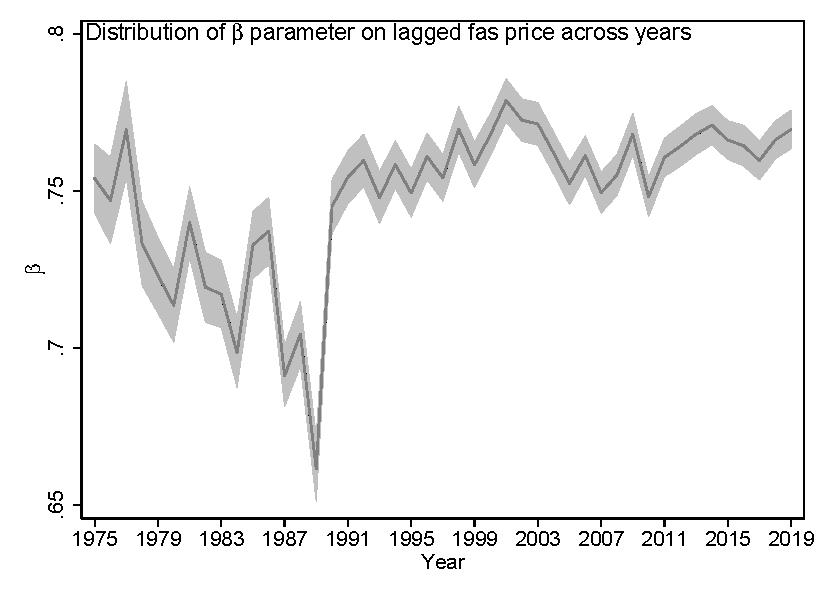
\includegraphics[width=3.2in, height=3.2in,keepaspectratio]{beta_lag_SITC5.pdf}
& 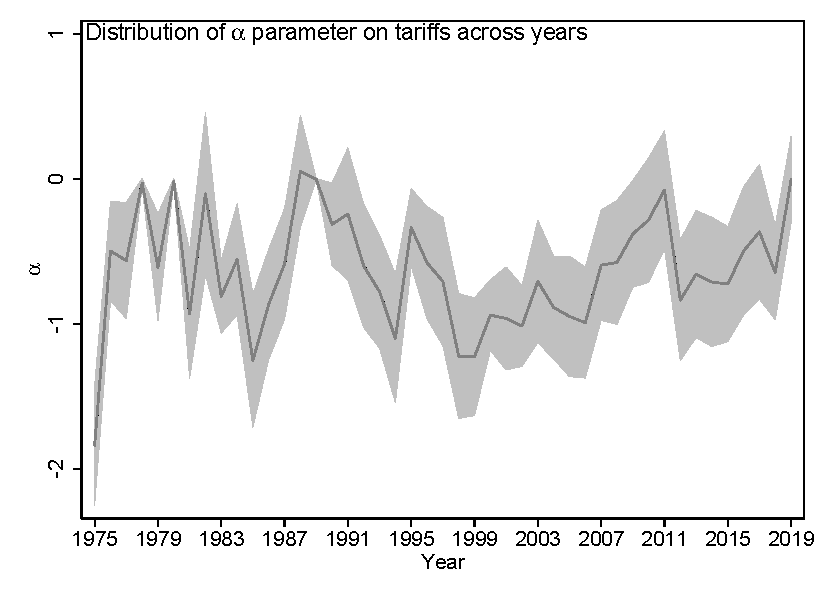
\includegraphics[width=3.2in,height=3.2in,keepaspectratio]{alpha_tariff_SITC5.pdf} \\
\end{tabular}
\end{center}
\end{figure}

%Staiger and Stock (1997) formalized the definition of “weak instruments” and most researchers seem to have concluded (incorrectly) from that work (orhearsay) that if the F-statistic on the excluded instruments in the first stage is greater than 10, one need worry no further about weak instruments.

%\newpage

Table \ref{tab: FS_sitc5} suggests that custom duties variations are a satisfactory predictor of fas prices $\widetilde{p}_{ik}$, with strong significance and the correct, negative sign. The lagged fas price $\log \widetilde{p}_{ikt-1}$ displays also the expected positive sign: with a $\beta$ parameter around 0.75 on average, fas prices exhibit substantial persistence. The F-statistic on the excluded instrument ($\frac{\Delta \tau^d_{is(k)t}}{1+\tau_{is(k)t-1}^d}$ ($\widehat{\alpha}$)) is on average above 10, the ``rule-of-thumb'' threshold value recommended by \cite{staiger_stock} as a test for weak instrumentation. In addition, Figure \ref{fig: FS_IV_SITC5} shows that most values of the $\alpha$ parameter stand between 0 and -1, as expected, except in a very small number of occasions, corresponding to abrupt fluctuations in oil prices. This is typically the case in 1975, with $\alpha$=-1.83. All in all, these estimates make us confident in the validity of our instrumentation strategy.



\paragraph{First-stage estimates based on HS10 data.}

Here we replicate our first-stage estimations using HS10 data, available between 2002 and 2019. In addition to one-year-lagged fas price, we use this time HS10-digit product-specific tariff duties. Table \ref{tab: FS_HS10} reports summary results of these first-stage regressions, while Figure \ref{fig: FS_IV_HS10} presents yearly estimates of $\beta$ and $\alpha$ parameters, together with 5\% confidence bands:


\begin{table}[htbp]\centering
\caption{Summary Results for First-Stage Regressions\label{tab: FS_HS10}}
\begin{tabular} {@{} l r r r r r r r @{}} \\ \hline
\textbf{variable } & \textbf{Mean} & \textbf{1\textsuperscript{st} Quart.} & \textbf{Median} & \textbf{3\textsuperscript{rd} Quart.} & \textbf{ S.D.} & \textbf{Min} & \textbf{Max} \\
\hline
$\log \widetilde{p}_{ikt-1}$ ($\widehat{\beta}$) &     0.7496 &     0.7453 &     0.7504 &     0.7539 &     0.0055 &     0.7385 &     0.7578 \\
 % sd_lag~t  &     0.0020 &     0.0020 &     0.0020 &     0.0021 &     0.0001 &     0.0019 &     0.0021 \\
Student t$_{\widehat{\beta}}$  &   369.81 &   361.19 &   366.34 &   376.77 &    12.91 &   352.61 &   395.33 \\
$\frac{\Delta \tau^d_{is(k)t}}{1+\tau_{is(k)t-1}^d}$ ($\widehat{\alpha}$)  &    -0.3612 &    -0.5636 &    -0.4175 &    -0.1918 &     0.3393 &    -0.9258 &     0.3448 \\
%  sd_tar~f  &     0.1511 &     0.1451 &     0.1618 &     0.1702 &     0.0325 &     0.0728 &     0.2011 \\
 Student t$_{\widehat{\alpha}}$   &    -2.2505 &    -3.3518 &    -2.5489 &    -1.3144 &     2.7027 &    -7.9494 &     4.7359 \\
  %  F_stat  &   6.85e+04 &   6.52e+04 &   6.71e+04 &   7.10e+04 &  4854.7592 &   6.22e+04 &   7.83e+04 \\
 F-statistic $\frac{\Delta \tau^d_{is(k)t}}{1+\tau_{is(k)t-1}^d}$ &    11.9399 &     1.7974 &     9.0342 &    14.8620 &    15.1916 &     0.8415 &    63.1932 \\
%  adj_r_~e  &     0.7697 &     0.7660 &     0.7691 &     0.7725 &     0.0068 &     0.7550 &     0.7826 \\
%  r_squa~n  &     0.5617 &     0.5591 &     0.5624 &     0.5661 &     0.0057 &     0.5505 &     0.5693 \\
\hline
%\multicolumn{8}{@{}l}{\footnotesize{\emph{Source:} C:\Users\coadministrateur\Dropbox\Papier_Lise_Guillaume\private\revision_JOEG\IV_rev/results/IV_referee1_yearly/FS_parameters_both_yearly_prod5_sect3.dta}}
\end{tabular}
\end{table}

\begin{figure}[htbp]
\caption{Yearly estimates of $\alpha$ and $\beta$ - HS10}\label{fig: FS_IV_HS10}
\begin{center}
\begin{tabular}{cc}
%{\small (A) $\beta$} & {\small (B) $\alpha$}\\
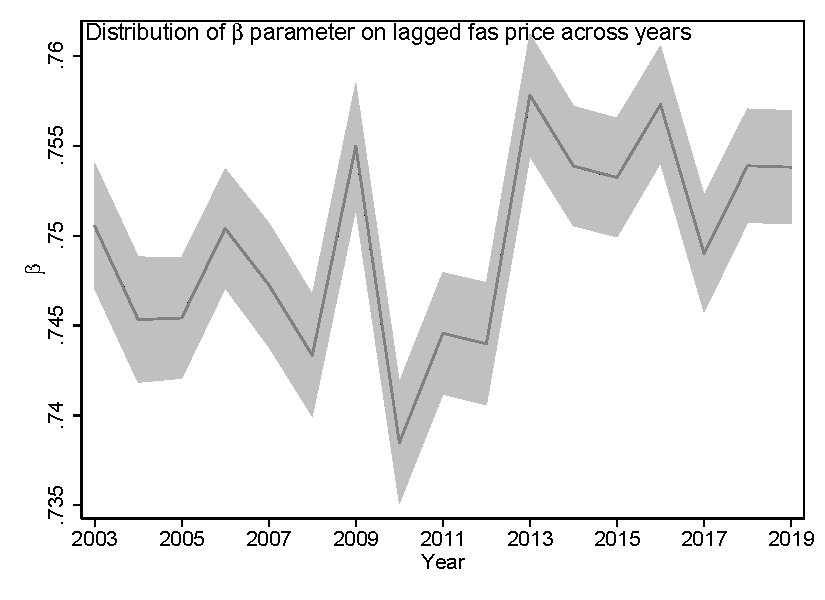
\includegraphics[width=3.2in, height=3.2in,keepaspectratio]{beta_lag_HS10.pdf}
& 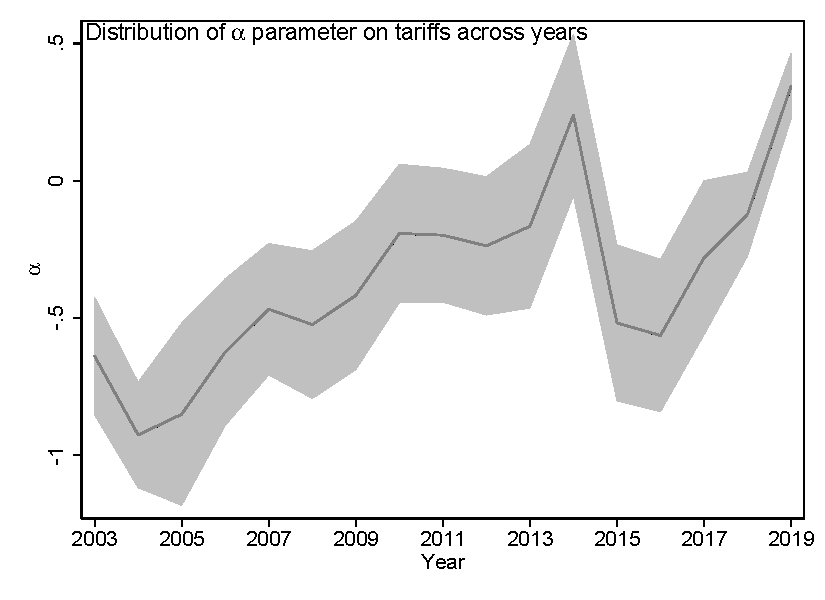
\includegraphics[width=3.2in,height=3.2in,keepaspectratio]{alpha_tariff_HS10.pdf} \\
\end{tabular}
\end{center}
\end{figure}

Results are qualitatively very similar to those reported on the longer-time-span, more-aggregated-SITC5 dataset previously reported. The F-statistic on the excluded instrument ($\frac{\Delta \tau^d_{is(k)t}}{1+\tau_{is(k)t-1}^d}$ ($\widehat{\alpha}$)) is on average close to 12, slightly higher than in our benchmark. As previously, Figure \ref{fig: FS_IV_HS10} shows that most values of the $\alpha$ parameter stand between 0 and -1, as expected, except in a few years which seem again to coincide with significant fluctuations in oil prices. Interestingly, the value of the $\alpha$ parameter is on average -0.36, lower than in our benchmark on SITC5 data. At this highly disaggregated level, pricing-to-market behavior seems less strong, indicating that the average firm is smaller than its average SITC5 counterpart. In addition, this average value is almost identical to the one found by \citet{Fontagne_Martin_Orefice2018} on French HS6 data between 1995 and 2010 (see the first-stage coefficients in their Table 6), or by \citet{Bussiere2013} on country-level data between 1980 and 2006. In any case, this strengthens our confidence in the validity of our estimation strategy.

\clearpage
\setcounter{table}{0}
\setcounter{figure}{0}
\renewcommand{\thefigure}{C.\arabic{figure}}
\renewcommand{\thetable}{C.\arabic{table}}




\section{Eliminating the composition effects: more details \label{app:comp-effects}}

In this section, we explain in more detail the method employed to eliminate the country and product dimensions of the estimated transport cost.

\subsection{More on our methodology}


\subsubsection{Estimation method for each additive and multiplicative component}

We begin by describing the estimation method to extract the fitted and unfitted series for both the additive and the multiplicative components, before turning to the `total costs'' series.
\smallskip

\paragraph{Obtaining the ``pure'' transport costs component series} - The empirical strategy to find the fitted transport cost measure (i.e. extracting from trade composition effect) can be described as a two-stage process.
First, we decompose the estimated measure in the three product/country/time dimensions, using fixed effects. In plain words, we measure how these costs have changed over time by blocking the composition of trade flows by product and country partners to the one observed in 1974 (the beginning of our sample).\smallskip

For the estimated ad-valorem component, we estimate the following equation:
\begin{eqnarray}
\ln(\widehat{\tau}_{ikt}-1)&=&\delta +\underbrace{\sum_{i \neq \text{ARG}}\alpha_i.\mathbbm{1}_i}_{(A)} + \underbrace{\sum_{s(k)\neq \text{011}}\beta_{s(k)}.\mathbbm{1}_{s(k)}}_{(B)} + \underbrace{\sum_{t \neq 1974}\gamma_t.\mathbbm{1}_t}_{(c)}+\epsilon_{ikt} \label{eq:compeffects_mult}
\end{eqnarray}

\noindent where $\mathbbm{1}_i$ and $\mathbbm{1}_{s(k)}$ represent country and sector fixed effects.\footnote{Throughout the exercise, we consider Argentina, the sector 011 and the first year of our dataset 1974, as references for the country, product and year dummies.}  Equation (\ref{eq:compeffects_mult}) is estimated using OLS, with a weighting scheme based on the value of each flow in the total value of flows for the relevant year.

In this exercise, we are interested in isolating the change in the time dimension of each transport cost component. This constitutes the second stage of our procedure. Based on Equation (\ref{eq:compeffects_mult}), we deduce after estimation that:

\[\left\{
  \begin{array}{lcl}
  \text{For the year 1974:} &&  \widehat{\tau}_{is74} -1 = \exp(\delta +\alpha_i+\beta_s), \\
  \text{For any year }t> 1974:&& \widehat{\tau}_{ist} -1 = \exp(\delta +\alpha_i+\beta_s)\times \exp(\gamma_t) \\
  \end{array}
\right.\]

From this, we obtain the following recursive link: $\widehat{\tau}_{ist} -1 = (\widehat{\tau}_{is74}-1)\exp(\gamma_t)$. Given the constraint $\tau>1$, we rewrite to get the percentage change between year 1974 and any year $t>1974$: $\Gamma_{ist} = 100.\frac{\widehat{\tau}_{ist}-1}{\widehat{\tau}_{is74}-1}  = 100\exp(\gamma_t)$. As such, the index of transport costs in year $t$ (relative to the reference year 1974) $\Gamma_{ist} $  only depends on the time trend, such that we can rewrite:
\begin{equation}
 \Gamma^{adv}_t= 100\exp(\gamma^{adv}_t)  \label{eq:tcadv_compoeffect}
\end{equation}

\noindent where the subscript $^{adv}$ clarifies that this time fixed effect is specific to the ad-valorem component. \medskip


As for the additive component, given that the sector fixed effect and the country fixed effect are additive rather than multiplicative by construction, we estimate the following equation using non-linear least squares:\footnote{For sake of notational simplicity, we do not distinguish the coefficients associated with the fixed effects between Equations (\ref{eq:compeffects_mult}) and (\ref{eq:compeffects_add}), even if they are specific to the type of transport costs considered (e.g. the series of $\gamma_t$ differs from one estimation to the other).
Note that we apply the same weighting scheme as for the OLS regression (based on the relative value of the flow).}

%, based on the additive cost series $\widehat{t}_{ikt}$ previously obtained:
\begin{eqnarray}
\ln(\widehat{t}_{ikt})&=&\ln\left( \delta + \underbrace{\sum_{i \neq \text{ARG}}  \alpha_i.\mathbbm{1}_i}_{(A)}+\underbrace{\sum_{s(k)}\beta_{s(k)}.\mathbbm{1}_{s(k)}}_{(B)}\right) + \underbrace{\sum_{t \neq 1974}\gamma_t.\mathbbm{1}_t}_{(c)}+\epsilon_{ikt} \label{eq:compeffects_add}
\end{eqnarray}



As displayed in Equations (\ref{eq:compeffects_mult}) and (\ref{eq:compeffects_add}), we decompose the estimated transport cost component in three elements: the country dimension (Term (A)), the product dimension (Term (B)) and the pure transport costs time trend (Term (c)).
Note that Equations (\ref{eq:compeffects_mult}) and (\ref{eq:compeffects_add}) preserve our specification of the ad-valorem and additive costs of Equations (\ref{eq:ad-valorem}) and (\ref{eq:add}), as we consider that the ad-valorem cost is the product of the country of origin and the goods dimension, while the additive cost is the sum of the two dimensions.
Both equations are estimated by transport mode.\smallskip

After estimating Equation (\ref{eq:compeffects_add}), we can rebuild the additive component according to:
\[\left\{
  \begin{array}{lcl}
\text{For the year 1974:}&&\widehat{t}_{is74}=  \delta + \alpha_i+ \beta_s, \\
\text{For any year}~t> 1974:&&\widehat{t}_{ist}=\left(\delta + \alpha_i+ \beta_s\right).\exp(\gamma_t)
\end{array}
\right.\]



From this, we deduce the recursive link: $\widehat{t}_{ist} = \widehat{t}_{is74} \times \exp(\gamma_t)$.

Given the constraint $t>0$, we then obtain the percentage change from 1974 from $\Gamma^{add}_{ist} = 100\frac{\widehat{t}_{ist}}{\widehat{t}_{ik74}} = 100\exp(\gamma_t)$. Again, it is independent of the product-origin country pair. We can thus rewrite the time-trend series for the additive transport cost component as:
\begin{equation}
\Gamma^{add}_t  = 100\exp(\gamma^{add}_t) \label{eq:tcadd_compoeffect}
\end{equation}




\noindent where the subscript $^{add}$ clarifies that this time fixed effect is specific to the additive component. However, one should notice that $\Gamma^{add}_t$ has been obtained considering the additive cost in USD, ie subject to the inflation trend. To eliminate the influence of inflation in the additive cost index, we extract the time trend (e.g, inflation) from the observed fas price series according to:
\begin{eqnarray}
\ln(\widehat{p}_{ikt})&=&\delta +\underbrace{\sum_{i \neq \text{ARG}}\alpha_i.\mathbbm{1}_i}_{(A)} + \underbrace{\sum_{s(k)\neq \text{011}}\beta_{s(k)}.\mathbbm{1}_{s(k)}}_{(B)} + \underbrace{\sum_{t \neq 1974}\gamma_t.\mathbbm{1}_t}_{(c)}+\epsilon_{ikt} \label{eq:compeffects_pfas}
\end{eqnarray}
Applying the same logic as above, we get $\Gamma^{\$}_t = 100\exp(\gamma^{\$}_t)$ where the subscript $^{\$}$ clarifies that this time fixed effect is specific to the inflation component of fas prices. We then eliminate the inflation trend in the additive cost index through:

\begin{equation}
\Gamma^{t/\widetilde{p}}_t  = 100 \frac{\Gamma^{add}_t}{\Gamma^{\$}_t} \label{eq:tsptilde_compoeffect}
\end{equation}

As a result, the two series $\Gamma^{adv}_t$ and $\Gamma^{t/\widetilde{p}}_t$ have a straightforward interpretation in percentage changes from the initial value of 100 for $t=1974$.



\paragraph{Obtaining the unfitted measures} The objective here is to express the unfitted transport cost component (additive and multiplicative) built as an index with reference value 100 in 1974, starting from the estimated values previously obtained ($\widehat{\tau}_t$, $\widehat{t}_t$, for each year $t$ from 1974 to 2019).
To do so, we apply the simple formula to get the following indices, for the ad-valorem and the additive cost components respectively:

$$\Gamma^{adv, raw}_t = 100\times\frac{\widehat{\tau}_t}{\widehat{\tau}_{1974}},\qquad \Gamma^{t/\widetilde{p}, raw}_t = 100\times\frac{\widehat{t}_t/\widetilde{p}_t}{\widehat{t}_{1974}/\widetilde{p}_{1974}}$$


\noindent recalling that the estimated series $\widehat{\tau}_t$, $\widehat{t}_t$ and the observed fas price series $\widetilde{p}_t$ are the weighted average series based on the value of each flow in the total value of flows for the relevant year (by transport mode).

\subsubsection{Estimation method for the total transport cost measures}

We also build two measures of the ``total'' transport costs for both the unfitted series and the pure transport cost series (i.e. composition effects excluded), with the objective to get a measure of total transport cost changes built as an index starting from the value 100 in 1974. Even if obeying the same logic, we proceed slightly differently for the unfitted and the fitted measures, as we now explain.
\smallskip

\paragraph{Obtaining the unfitted total transport cost index} For each transport mode, we build the total transport cost series based on Equation (\ref{eq:base_estimee}) according to:
$$\widehat{TC}^{raw}_t= \widehat{\tau}^{adv}_t -1 + \frac{\widehat{t}_t}{\widetilde{p}_t}$$
\noindent where $\widehat{\tau}^{adv}_t$ and $\widehat{t}_t$ are the weighted average values over the country/sector dimension estimated (conditional on a year and a transport mode), as explained in Section \ref{sec:data_method}, and $\widetilde{p}_t$ the corresponding weighted average observed fas price.
We then transform this value in an index with base year 1974, applying a similar formula as above (by transport mode):
%$$\Gamma^{tc, raw}_t = 100\frac{\widehat{tc}^{raw}_t -1 }{\widehat{tc}^{raw}_{1974}-1}$$

$$\Gamma^{tc, raw}_t = 100\frac{\widehat{TC}^{raw}_t  }{\widehat{TC}^{raw}_{1974}}$$



\paragraph{Obtaining the fitted total transport cost index} The same logic as above applies to constructing the fitted measure of total transport cost (i.e. composition effect excluded), with one notable exception: Fitted ad-valorem and additive components have not been estimated in value, but extracted and built as indices. In a first step then, starting from these indices, we rebuild the fitted measures of each transport cost component in value (expressed in percentage of the fas price in both cases):

\begin{eqnarray*}
\widehat{\tau}^{pure, adv}_t -1 &=&\Gamma^{adv}_t \frac{\bar{\tau}_{1974} }{100} \\
\widehat{t}^{pure}_t &=& \Gamma^{add}_t\frac{\bar{t}_{1974}}{100}
\end{eqnarray*}



\noindent with $\bar{\tau}_{1974} = \exp(\delta + \sum_i \alpha_i + \sum_s \beta_s)$ the (weighted) mean ad-valorem transport cost in 1974 (based on Equation (\ref{eq:compeffects_mult})) and $\bar{t}_{1974} = \delta + \sum_i \alpha_i + \sum_s \beta_s$ the (weighted) mean additive transport cost in 1974 (based on Equation (\ref{eq:compeffects_add})). We then deduce the fitted value of the overall cost according to:
$$\widehat{TC}^{pure}_t= \widehat{\tau}^{pure, adv}_t -1 + \frac{\widehat{t}^{pure}_t}{\widetilde{p}_t}$$

Last, we transform this (fitted) measure of total transport cost in an index with base year 1974, applying a similar formula as above (by transport mode):
$$\Gamma^{tc}_t = 100\frac{\widehat{TC}^{pure}_t}{\widehat{TC}^{pure}_{1974}}$$


\subsection{Comparing with \cite{hummels2007} \label{app:compare_Hummels}}

In this section, we investigate the difference of results with \cite{hummels2007} regarding the importance of the composition effects in characterizing the time trends of international transport costs.
In order to do so, we start from the empirical specification implemented by \cite{hummels2007} (also making use of Hummels' Stata codes provided on his webpage\footnote{\url{http://www.krannert.purdue.edu/faculty/hummelsd/research/jep-transport-cost-data.php}}), to better identify the precise points of difference between our estimation strategies.

Let us start from Hummels' (2007) quotation (p.
146) according to which (for air), the ``\textit{unadjusted measure of ad valorem air shipping costs [is] the aggregate expenditures on air shipping divided by the value of airborne imports}''.
From this, we get the ``raw'' ad-valorem measure of transport costs as the ratio between the imported total value and the exported total value ($(p_{ikt} - \widetilde{p}_{ikt})q_{ikt}/\widetilde{p}_{ikt}q_{ikt})$, the mean yearly value being obtained by weighting each flow by its value in total trade flows (ie, yielding the observed aggregate value of $\tau_t$ for air).

Consider now the ``fitted ad-valorem rate''.
\cite{hummels2007} uses ``\textit{a regression in which the dependent variable is the ad-valorem air freight cost in logs for commodity $k$ shipped from exporter} $i$\footnote{To be consistent with our notations, we change the country subscript from $j$ (Hummels, 2007 terminology) to $i$ (our terminology).} \textit{at time $t$.
The independent variables include a separate intercept for each exporter-commodity shipped, the weight/value ratio in logs for each shipment, and year dummy variables}''.
With the value of the shipment equal to $\widetilde{p}_{ikt}q_{ikt}$, and denoting the air freight cost as $TC_{ikt}$, we can formulate the above sentence according to the following equation (suppressing the transport mode index to alleviate notation):

\begin{eqnarray}
&&\ln TC_{ikt} = \delta+ \beta \ln \frac{q_{ikt}}{\widetilde{p}_{ikt}q_{ikt}} + \sum_{i,k}\alpha_{ik}.\mathbbm{1}_{ik}+ \sum_{t}\gamma_{t}.\mathbbm{1}_{t} + \epsilon_{ikt} \notag \\
\Leftrightarrow && \ln TC_{ikt} = \delta+ \beta \ln \frac{1}{\widetilde{p}_{ikt}} + \sum_{i,k}\alpha_{ik}.\mathbbm{1}_{ik}+ \sum_{t}\gamma_{t}.\mathbbm{1}_{t} + \epsilon_{ikt} \label{eq:Hummels1}
\end{eqnarray}

\noindent where $TC_{ikt}$ is measured by the ratio between freight charges, i.e.
$(p_{ikt} - \widetilde{p}_{ikt})q_{ikt}$ and the value of the shipment, i.e.
$\widetilde{p}_{ikt}q_{ikt}$, or equivalently : $TC_{ikt} = \frac{p_{ikt} - \widetilde{p}_{ikt}}{\widetilde{p}_{ikt}}$.\medskip

After estimating Equation (\ref{eq:Hummels1}), \cite{hummels2007} uses the predicted value of the regression, denoted $\widehat{TC}_{ikt}$, to obtain the unweighted average in the product/origin country dimension $i,k$, denoted $\widehat{TC}_{t}$, to be compared to the unfitted ad-valorem rate $TC_{t}$ (by transport mode).\medskip

What are the main differences with our estimation strategy? Five points may be underlined.
First, \cite{hummels2007} obtains the fitted ad-valorem rate in one step (considering the observed export-import price gap on the left-hand side of Equation (\ref{eq:Hummels1})), while we use our two-step approach to extract the fitted transport cost (ie, composition effect excluded) from the (already estimated) unfitted rate.
However, this is a slight difference, as in both cases it ultimately amounts to taking the predicted value of Equation (\ref{eq:Hummels1}) (which eliminates the changes specific to the origin country/product/year triplet).
Second, in contrast to us, \cite{hummels2007} does not purge his measure of the fitted ad-valorem rate by the country-sector fixed effects.
This is not likely to make a substantial difference, however, as these fixed effects are by nature constant over time. Accordingly, they only amount to a scale effect.
%Accordingly, \textbf{they only amount to a scale effect. - rather than \textit{they only play as a scale effect as the estimate is in log}. A-t-on besoin de dire que c'est en log?}.

A third difference is that we separate the country-product fixed effects ($\sum_{i,k}\alpha_{ik}.\mathbbm{1}_{ik}$ in Equation (\ref{eq:Hummels1})) into two separate components (origin country and product dimensions).
As discussed in Section \ref{sec:robustness}, this is constrained by the number of fixed effects to estimate.
However, we do not view this as the major cause of difference between our two methods, as can be inferred from the robustness analysis on this point in Section \ref{sec:robustness}.

Fourth, we differ in the weighting scheme retained to obtain the yearly value of the fitted transport cost (in the terms of \cite{hummels2007} method, the switch from $\widehat{TC}_{ikt}$ to $\widehat{TC}_{t}$). \cite{hummels2007} takes the unweighed average value over the $i,k$ dimension, which implicitly attributes a weight equal to 1 to each flow. We proceed differently, as we weight each flow by its relative value on total trade flows (on the relevant year of observation), based on the argument that this weighting scheme does not overweight the small flows in value. However, we ensure that our results are not sensitive to an alternative weighting scheme, by building the average fitted transport costs rate as in \cite{hummels2007}, as reported in the following Section \ref{app:compeffects_weights}.

One last difference remains to be commented, concerning the way the additive component of international transport costs is treated.
As we show below, it turns out to be key in accounting for the difference of results with \cite{hummels2007}.
Coming back to Equation (\ref{eq:Hummels1}), it can be shown that it encompasses the two extreme cases of only ad-valorem costs ($\beta = 0$) and only additive costs ($\beta=1$), as also pointed out in \cite{hummels_skiba}. Rewriting the predict of Equation (\ref{eq:Hummels1}) in a simpler form as:

$$\ln TC_{ikt} \equiv \ln \left(\frac{p_{ikt}- \widetilde{p}_{ikt}}{\widetilde{p}_{ikt}} \right) = \Delta_{ikt}- \beta \ln \widetilde{p}_{ikt} $$

\noindent where $\Delta_{ikt} \equiv \sum_{i,k}\alpha_{ik}.\mathbbm{1}_{ik}+ \sum_{t}\gamma_{t}.\mathbbm{1}_{t}$ agglomerates the various fixed effects for reading clarity.

Under the first polar case with $\beta = 1$, it becomes:
\begin{eqnarray*}
&&\ln \left(\frac{p_{ikt}- \widetilde{p}_{ikt}}{\widetilde{p}_{ikt}} \right) = \Delta_{ikt}- \ln \widetilde{p}_{ikt} \\
\Leftrightarrow && \ln (p_{ikt}- \widetilde{p}_{ikt}) = \Delta_{ikt}
\end{eqnarray*}
\noindent Taken the exponential, this becomes: $p_{ikt} = \widetilde{p}_{ikt} + \exp(\Delta_{ikt})$ or, equivalently: $p_{ikt} = \widetilde{p}_{ikt} + t_{ikt}$, with $t_{ikt}$ appropriately defined. This exactly corresponds to the case of additive costs only.

In the second polar case with $\beta = 0$, Equation (\ref{eq:Hummels1}) becomes:
$$\ln \left(\frac{p_{ikt}}{\widetilde{p}_{ikt}}-1\right) = \Delta_{ikt}$$

Taking the exponential, we get: $\frac{p_{ikt}}{\widetilde{p}_{ikt}}  = \exp (\Delta_{ikt})+1$, that is: $p_{ikt} = \tau_{ikt} \widetilde{p}_{ikt}$, with $\tau_{ikt}$ appropriately defined. This exactly corresponds to the case of ad-valorem transport costs only.


As noted by \cite{hummels_skiba}, $0<\beta<1$ represents the elasticity of freight costs to the export prices, increasing with the relative weight of the additive component in international transport costs.
By estimating Equation (\ref{eq:Hummels1}) with a constant $\beta$, \cite{hummels2007} assumes that the share of additive costs does not vary over time, country partner or product.
This is an important difference with our method, as we measure transport costs by explicitly allowing for an additive component that varies in the three dimensions (i.e. allowing for a varying $\beta$ across time, country partner and product). We suspect this to be the key driver between Hummels's results and ours regarding the time trend in the trade composition effects. To establish this point clearly, we replicate the method adopted by \cite{hummels2007}, outlined above, on our database (which is the same as his until 2004).
The results are reported in Figure \ref{fig:comp_effects_as_in_Hummels}.


\subsection{Robustness to the weighting scheme \label{app:compeffects_weights}}

When aggregating the trade cost measure over the product/country ($i,k$) dimension, \cite{hummels2007} takes the unweighted average value over the $i,k$ dimension, which implicitly attributes a weight equal to 1 to each flow.
Our benchmark specification  (at the root of Figure \ref{fig:totalTC_compeffects_excl}) proceeds differently, as each flow is weighted by its relative value in total trade flows. In this section, we check whether this difference of treatment is responsible or not for the difference in results relative to the role of the trade composition effects, which we rather attribute to the modeling of the additive component.

To this aim, we rebuild the fitted values for each of our transport cost measures (ad-valorem, additive and overall) applying the \cite{hummels2007} weighting scheme (i.e. taking the unweighed average value over the $i,k$ dimension), which we then express as indices, with the reference value 100 in 1974.
The results are reported in Figure \ref{fig:compeffects_robustness}.

\begin{figure}[htbp]
\caption{Transport cost time trends: robustness to the weighting scheme}
\label{fig:compeffects_robustness}
\begin{center}
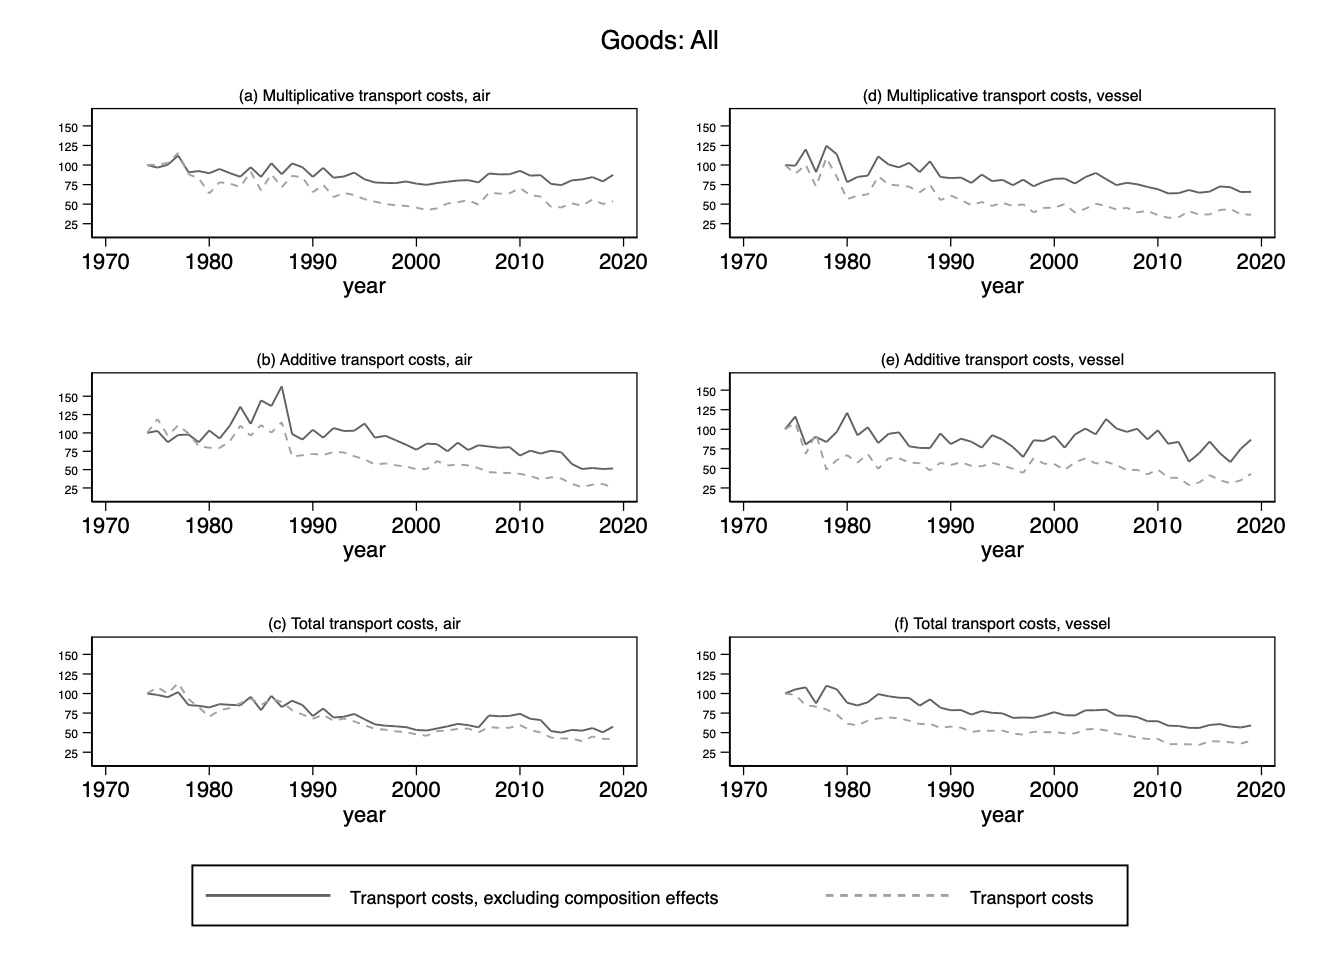
\includegraphics[height=8cm]
{graph_composition_all_np.jpg}
\end{center}
\end{figure}

The comparison of Figure \ref{fig:compeffects_robustness} (applying Hummels's weighting scheme) and Figure \ref{fig:totalTC_compeffects_excl} (applying our weighting scheme) prompts two comments.
First, differences do show up, in particular for the multiplicative component of air transport.
This suggests that the weighting scheme is not innocuous in the time trend decomposition exercise.
However, Figure \ref{fig:compeffects_robustness} also shows that the composition effects have contributed to strengthen the decrease in the ``ceteris paribus'' transport costs in air transport (in Figure \ref{fig:compeffects_robustness}, panel (A), overall transport costs have decreased more than the fitted component). This stands in accordance with the conclusions drawn from Figure \ref{fig:totalTC_compeffects_excl}, rather than partly offsetting this decline, as argued by \cite{hummels2007}. These results confirm that it is the functional form and precisely the modeling of the additive component, rather than the weighting scheme, that is key in understanding the underlying determinants of the overall transport costs time trends, as pointed out in Section \ref{sec:results_trends}.


\section{More on the model \label{app:theoretical_model}}

\subsection{The model in the general case}

In this section, we provide more details on the model's solving in the general case, i.e. without specifying any functional form for the distribution of firm productivity.

\subsubsection{Firms}

\paragraph{Profit-maximizing behavior}

On the domestic market, the objective is to maximize profit $\pi_d(\omega)= \left(p^d(\varphi) -\frac{1}{\varphi}  \right)c(\varphi)$, taking into account the consumer demand function $c(\varphi) = \left(\frac{p(\varphi)}{P}  \right)^{-\sigma} \frac{E}{P}$. In a monopolistic set-up, each firm (of productivity $\varphi$) is the sole producer of variety $\omega$, implying a one-to-one link between $\omega$ and $\varphi$, such that we could write $\omega(\varphi)$. For sake of notational simplicity, we omit this link and simply write the consumer demand function as a function of $\varphi$ directly.
The optimal pricing behavior yields:
$$p_d(\varphi) = \frac{\sigma}{\sigma-1}\frac{1}{\varphi}$$
With a CES specification on household's preferences, the firm sets its price as a constant mark-up on marginal cost, which is inversely related to its productivity as for the domestic market. \medskip

Conditional on exporting abroad, the profit-maximizing program on the export market requires the inclusion of variable international trade costs. The optimizing program accordingly rewrites as:
\begin{eqnarray*}
\max_{p_x(\varphi)} \pi_x(\varphi) &=& \left(p_x(\varphi) -\frac{\tau}{\varphi}  \right)c_x(\varphi) - tc_x(\varphi) \\
\text{s.t. }&&c_x(\varphi) = \left(\frac{p_x(\varphi)}{P^\ast}  \right)^{-\sigma} \frac{E^\ast}{P^\ast}
\end{eqnarray*}

\noindent where $E^\ast$ and $P^\ast$ refer to nominal expenditures and the price index in the foreign country, $c_x(\omega)$ to the demand for variety $\omega$ from the Foreign household and $p_x(\omega)$ to the price set by the firm producing the variety $\omega$ on the export market. Solving for this yields:
\begin{equation}
p_x(\varphi) = \frac{\sigma}{\sigma-1}\left[\frac{\tau}{\varphi} +t \right] \label{eq:px}
\end{equation}

Making use of the firm's first-order pricing conditions, revenues on each local and export market respectively read as:
\begin{eqnarray}
% \nonumber % Remove numbering (before each equation)
  r_d(\varphi) &=& \left[\frac{1}{\rho \varphi}  \right]^{1-\sigma} P^{\sigma-1} E \label{eq:rd}\\
  r_x(\varphi) &=& \left[\frac{1}{\rho}\left(\frac{\tau}{\varphi} +t\right)  \right]^{1-\sigma} P^{\sigma-1} E \label{eq:rx}
\end{eqnarray}
\noindent with $\rho =  \frac{\sigma-1}{\sigma}$ inversely related to the markup rate.

\paragraph{Zero-cutoff profit conditions} With $\frac{\pi_d(\varphi^\ast)}{\delta}$ and  $\frac{\pi_x(\varphi_x^\ast)}{\delta}$ the expected profit on the domestic and export market respectively, the zero cut-off (ZCP) productivity levels for successful entry on each market should verify:
\begin{eqnarray*}
\frac{\pi_d(\varphi^\ast)}{\delta} = 0 &\Leftrightarrow & \varphi^\ast = \frac{1}{f^{\frac{1}{1-\sigma}}B^{\frac{-1}{1-\sigma}}}\\
\frac{\pi_x(\varphi_x^\ast)}{\delta} = 0 &\Leftrightarrow & \varphi_x^\ast = \frac{\tau}{f_x^{\frac{1}{1-\sigma}}B^{\frac{-1}{1-\sigma}} -t}
\end{eqnarray*}

\subsubsection{Aggregation: Price indices}


Following \cite{melitz}, and decomposing the set of available varieties into $\Omega_d$, $\Omega_x$ the set of varieties respectively produced at Home and imported, one can rewrite the price index as:
\begin{eqnarray*}
P &=& \left[\int_{\omega \in \Omega_d} p_d^{1-\sigma}(\omega)d\omega + \int_{\omega \in \Omega_x} p_x^{1-\sigma}(\omega)d\omega  \right]^{\frac{1}{1-\sigma}} \\
&=& \left[\int_{0}^\infty p_d^{1-\sigma}(\varphi)M\mu(\varphi)d\varphi + \int_{0}^\infty p_x^{1-\sigma}(\varphi)M_x \mu_x(\varphi)d\varphi  \right]^{\frac{1}{1-\sigma}}
\end{eqnarray*}
Making use of Equation (\ref{eq:muofphi}), the price index reads as:
\begin{eqnarray*}
P &=& \left[\frac{M}{1-G(\varphi^\ast)}\int_{\varphi^\ast}^\infty p_d^{1-\sigma}(\varphi)g(\varphi)d\varphi + \frac{M_x}{1-G(\varphi_x^\ast)}\int_{\varphi^\ast_x}^\infty p_x^{1-\sigma}(\varphi)g(\varphi)d\varphi  \right]^{\frac{1}{1-\sigma}} \\
\text{with}&& \left\{
\begin{array}{lll}
p_d(\varphi)&=& \frac{\sigma}{\sigma-1} \frac{1}{\varphi}\\
p_x(\varphi)&=& \frac{\sigma}{\sigma-1} \left[\frac{\tau}{\varphi} +t\right]
\end{array}
\right.
\end{eqnarray*}
Accordingly, the price index can be rewritten as:
$$P = \left(\frac{\sigma}{\sigma-1}\right)\left[\frac{M}{1-G(\varphi^\ast)}\int_{\phi^\ast}^\infty \phi^{\sigma-1}g(\varphi)d\varphi + \frac{M_x}{1-G(\varphi_x^\ast)}\int_{\varphi^\ast_x}^\infty \left[\varphi \left(\frac{\tau}{\tau+t \varphi}  \right)  \right]^{\sigma-1}g(\varphi)d\varphi  \right]^{\frac{1}{1-\sigma}}$$


Similarly as in the closed-economy case (\cite{melitz}), let us define $\widetilde{\varphi}(\varphi^\ast)$ and $\widetilde{\varphi}_x(\varphi_x^\ast)$ as the weighted average of productivities of the domestic firms, on the domestic market and the export market respectively:\footnote{In the symmetric two-country model, $\widetilde{\varphi}_x(\varphi_x^\ast)$ also corresponds to the weighted average of productivities of foreign exporters at Home, e.g. associated with the imported varieties.}

\begin{eqnarray}
\widetilde{\varphi} &=& \left[\frac{1}{1-G(\varphi^\ast)}\int_{\varphi^\ast}^\infty \phi^{\sigma-1}g(\varphi)d\varphi   \right]^{\frac{1}{\sigma-1}} \label{eq:def_phitilde}\\
\widetilde{\varphi}_x &=& \left[\frac{1}{1-G(\varphi_x^\ast)}\int_{\varphi^\ast}^\infty \left[\varphi\left(\frac{\tau}{\tau+t \varphi}  \right) \right]^{\sigma-1}g(\varphi)d\varphi   \right]^{\frac{1}{\sigma-1}} \label{eq:def_phitildex}
\end{eqnarray}



Further defining $M_T = M+M_x$ as the total number of varieties accessible to the consumers, one can show that the consumer price index can be rewritten as: comes that:
$$P = \frac{\sigma}{\sigma-1}M_T^{\frac{1}{1-\sigma}}\left[\frac{1}{M_T}\left(M\widetilde{\varphi}^{\sigma-1} + M_x \left( \frac{\widetilde{\varphi}_x}{\tau} \right)^{\sigma-1} \right)  \right]^{\frac{1}{1-\sigma}}$$

\noindent with $\widetilde{\varphi}(\varphi^\ast)$ and $\widetilde{\varphi}_x(\varphi_x^\ast)$ the weighted average of productivities of domestic and imported varieties respectively defined in Equations (\ref{eq:def_phitilde}) and (\ref{eq:def_phitildex}). With $\widetilde{\varphi}_T \equiv \left[\frac{1}{M_T}\left(M\widetilde{\varphi}^{\sigma-1} + M_x \left( \frac{\widetilde{\varphi}_x}{\tau} \right)^{\sigma-1} \right)  \right]^{\frac{1}{1-\sigma}}$ the weighted average of firm productivities on the domestic market (including both local producers and foreign producers exporting at Home), the price index can be expressed as $P = M_T^{\frac{1}{1-\sigma}}\frac{1}{\rho \widetilde{\varphi}_T }$. As in \cite{melitz}, given our assumptions of wage normalization and a one-sector economy, welfare per worker is simply equal the inverse of the price level: $\mathcal{W} = \frac{w}{P}= P^{-1}$, leading to:

\begin{equation*}
\mathcal{W} = \rho \widetilde{\varphi}_T M_T^{\frac{1}{\sigma-1}}
\end{equation*}
\noindent that is, Equation (\ref{eq:Welfare}).

\paragraph{Free-entry condition} In the open-economy setting, the free-entry condition is given by:
\begin{equation*}
  \sum_{t=0}^{\infty}(1-\delta)^t \left(\int_{\varphi^\ast}^{\infty} \pi_d(\varphi )dG(\varphi) + \int_{\varphi_x^\ast}^{\infty} \pi_x(\varphi )dG(\varphi)  \right) = f_e
\end{equation*}
$\bar{\pi}$ can be expressed as $\bar{\pi} =\pi_d(\widetilde{\varphi}(\varphi^\ast)) + \rho_x \pi_x(\widetilde{\varphi}_x(\varphi_x^\ast))$, with $\pi_d(\widetilde{\varphi}(\varphi^\ast)) \equiv \bar{\pi}_d$ the average expected profit on the domestic market, $\pi_x(\widetilde{\varphi}_x(\varphi_x^\ast))\equiv \bar{\pi}_x$ the average expected export profit and $\rho_x$ the probability of exporting (conditional on entry on the domestic market), equal to $\rho_x = \frac{1-G(\varphi_x^\ast)}{1-G(\varphi^\ast)}$.

Noticing that, from Equation (\ref{eq:rd}), $\frac{r_d(\varphi)}{r_d(\varphi^\ast)} = \left( \frac{\varphi}{\varphi^\ast} \right)^{\sigma-1}$ and similarly on the export market, Equations (\ref{eq:pid_rd}) and (\ref{eq:pix_rx}) can be rewritten as:
\begin{eqnarray*}
\bar{\pi}_d &=& \left\{\left(\frac{\widetilde{\varphi}^\ast}{\varphi^\ast}\right)^{\sigma-1}-1 \right\}f \\
\bar{\pi}_x &=& \left\{\left[\left(\frac{\widetilde{\varphi}_x^\ast}{\varphi_x^\ast}\right)\left(\frac{\tau+ t \varphi^\ast_x}{\tau+ t \widetilde{\varphi}^\ast_x}\right)\right]^{\sigma-1}-1 \right\}f_x
\end{eqnarray*}

Making use of the above elements, we finally get the zero-cut off profit condition in the open economy with additive costs as:


\subsubsection{Solving the general equilibrium}

Following \cite{melitz} and the subsequent literature, denoting $M_e$ the mass of prospective entrants and $\rho_e$ the probability of successful entry (equal to $1-G(\varphi^\ast)$), considering only steady-state equilibrium needs to verify the entry-exit flow equilibrium condition:
$$\rho_e M_e = \delta M$$.

Given the wage normalization, total revenue in each country should be such that: $E = L_p+\Pi$, with $L_p$ the number of workers of the productive sector and $\Pi$ total profits. Labor market equilibrium further requires: $L = L_p+ L_e$ with $L_e = f_eM_e$ as sunk entry costs are paid in terms of labor. Combining this with the free-entry condition (\ref{eq:FEC}), we obtain that $\Pi = L_e$: Total profits in the productive sector are used to pay the entry sunk costs. Making use of this, we obtain that aggregate income in each country is equal to its labor endowment: $E =L$.

Further, total revenue can de expressed as the product of the average sales and the mass of active producers, according to: $E = M\bar{r}$, with $\bar{r}$ average sales. Similarly as for profits, it can be expressed as the sum of average sales on each local and foreign market:
$$\bar{r} = r_d(\widetilde{\varphi}(\varphi^\ast))+ \rho_x r_d(\widetilde{\varphi}_x(\varphi_x^\ast))$$
\noindent with the (conditional) probability of export $\rho_x = \frac{1-G(\varphi^\ast_x)}{1-G(\varphi^\ast)}$ and average sales on each market which can be shown to be:
\begin{eqnarray*}
\bar{r}_d &=& \left(\frac{\widetilde{\varphi}^\ast}{\varphi^\ast}\right)^{\sigma-1} \sigma f \\
\bar{r}_x &=& \left(\frac{\widetilde{\varphi}_x^\ast}{\varphi_x^\ast}\right)^{\sigma-1}\left(\frac{\tau+ t \varphi^\ast_x}{\tau+ t \widetilde{\varphi}^\ast_x}\right)^{\sigma-1} \sigma f_x
\end{eqnarray*}

Given selection on the export market, the mass of domestic exporters depends on that of domestic active firms according to: $M_x = \rho_x M$. In the symmetric equilibrium, the total mass of available varieties is then: $M_T= M+M_x = (1+\rho_x)M$.

\subsubsection{Summary}

Equations (\ref{eq:def_phitilde}), (\ref{eq:def_phitildex}), (\ref{eq:ZCP}), (\ref{eq:link_thresholds}) and (\ref{eq:FEC}) determine a system of interdependent equations in five endogenous variables $\left\{\bar{\pi}, \widetilde{\varphi}, \widetilde{\varphi}_x, \varphi^\ast, \varphi^\ast_x \right\}$. We can deduce the equilibrium values of the remaining set of variables $\left\{P, M_T, M, M_x, \widetilde{\varphi}_T, \bar{r} \right\}$ by recursively solving the following set of equations:

\begin{eqnarray*}
% \nonumber % Remove numbering (before each equation)
 \bar{r}&=& \left(\frac{\widetilde{\varphi}^\ast}{\varphi^\ast}\right)^{\sigma-1} \sigma f + \frac{1-G(\varphi^\ast_x)}{1-G(\varphi^\ast)}\left(\frac{\widetilde{\varphi}_x^\ast}{\varphi_x^\ast}\right)^{\sigma-1}\left(\frac{\tau+ t \varphi^\ast_x}{\tau+ t \widetilde{\varphi}^\ast_x}\right)^{\sigma-1} \sigma f_x \\
 M &=& \frac{L}{\bar{r}} \\
M_x &=& \frac{1-G(\varphi^\ast_x)}{1-G(\varphi^\ast)} M \\
M_T &=& \left(1+ \frac{1-G(\varphi^\ast_x)}{1-G(\varphi^\ast)} \right)M \\
\widetilde{\varphi}_T &=& \widetilde{\varphi}_T \equiv \left[\frac{1}{M_T}\left(M\widetilde{\varphi}^{\sigma-1} + M_x \left( \frac{\widetilde{\varphi}_x}{\tau} \right)^{\sigma-1} \right)  \right]^{\frac{1}{1-\sigma}} \\
P &=& M_T^{\frac{1}{1-\sigma}} \frac{\rho}{\widetilde{\varphi}_T}
\end{eqnarray*}


\subsection{With a Pareto distribution}


As in most of the related literature (\cite{Irrazabal_2015}, \cite{melitz-redding-Handbk-IT-2014}, \cite{ghironi}), we adopt a Pareto distribution for firm productivity heterogeneity, with the density and the cumulative functions respectively written as:
\begin{eqnarray*}
g(\varphi) &=& k\varphi_{\text{min}}^k \varphi^{-(k+1)}\\
G(\varphi) &=& 1 -\left( \frac{\varphi_{\text{min}}}{\varphi} \right)^k
\end{eqnarray*}

With the Pareto distribution, the system of Equations (\ref{eq:def_phitilde}), (\ref{eq:def_phitildex}), (\ref{eq:ZCP}), (\ref{eq:link_thresholds}) and (\ref{eq:FEC}) can be rewritten as a system of four equations in four endogenous variables: $\left\{\bar{\pi}, g(\varphi_x^\ast),\varphi_x^\ast, \varphi^\ast  \right\}$ as given by:

\begin{eqnarray}
\bar{\pi}&=& \kappa f + \left(\varphi^\ast \right)^k f_x\left[k\left(\frac{\tau}{\varphi_x^\ast}+t  \right)^{\sigma-1}\left[  1+(k(\varphi_x^\ast)^k g(\varphi_x^\ast))^{\frac{1}{\sigma-1}}\right]^{1-\sigma}  - \left( \varphi_x^\ast \right)^{-k} \right] \label{eq:systemPareto_1}\\
g(\varphi_x^\ast)&=&\int_{\varphi_x^\ast}^\infty \varphi^{\sigma-1-(k+1)}(\tau +t\varphi)^{1-\sigma}d\varphi \label{eq:systemPareto_2} \\
\frac{\varphi_x^\ast}{\tau+ t\varphi_x^\ast}&=&\varphi^\ast \left[ \frac{f}{f_x} \right]^{\frac{1}{1-\sigma}} \label{eq:systemPareto_3}\\
\bar{\pi}&=& \delta f_e \left( \frac{\varphi^\ast}{\varphi_{\text{min}}} \right)^k \label{eq:systemPareto_4}
\end{eqnarray}

\noindent with $\kappa \equiv \frac{\sigma-1}{k-(\sigma-1)}$. Notice that, in the absence of additive costs ($t=0$), Equation (\ref{eq:systemPareto_2}) rewrites as:
$$g(\varphi_x^\ast) = \tau^{1-\sigma}\left[ \frac{(\varphi_x^\ast)^{-(k-(\sigma-1))}}{k-(\sigma-1)}\right]$$
The system of Equations (\ref{eq:systemPareto_1})-((\ref{eq:systemPareto_4}) thus simplifies to be solved recursively with a full analytical solution. This is no longer the case in the presence of additive costs, and we have to rely on the model's simulations to obtain the general equilibrium of the model for a given calibration of the deep parameters.


\subsection{Some extra theoretical results}

In this section, we run an additional exercise to confirm the importance of the additive dimension in the welfare-detrimental effects of trade costs. Under a constant fixed export costs, we simulate the model under two alternative cases. Starting from the values observed in 1974, we simulate \textit{(i)} the observed reduction in the additive cost $t/\widetilde{p}^fas$, maintaining the ad-valorem component at its initial (1974) value (Scenario (A)), and  \textit{(ii)} the opposite case where $\tau$ takes its 2019 value with the same additive cost (in percentage of the fas price) as in 1974 (Scenario (B)). These two scenarios (as well as the initial one based on 1974 values) are reported in Table \ref{tab:calib_TC_appendix}.


\begin{table}[htb]
  \centering
  \caption{Exploring alternative scenarios: Calibration }\label{tab:calib_TC_appendix}
\begin{center}
	\begin{tabular}{l|c|cc||c|cc}
\hline \hline
& \multicolumn{3}{|c||}{Air transport} & \multicolumn{3}{|c}{Vessel transport} \\ \hline
& 1974 & \multicolumn{2}{|c||}{2019} & 1974 & \multicolumn{2}{|c}{2019}\\ \cline{2-7}
Scenario &  & (A) &  (B) &  & (A) & (B) \\ \hline
$\tau$ (in \% of fas price) & 3.87 & 3.87 & 1.92 & 5.58 & 5.58 & 2.05\\
$t/\widetilde{p}^{\text{fas}}_x$ (in \% of fas price) & 2.42 & 0.57 & 2.42 & 2.97 & 1.6 & 2.97 \\
TC (in \% of fas price) & 6.29 & 4.44 & 4.34 & 8.55 & 7.18 & 5.02 \\
$\beta$ (in \%) & 38.5 & 12.84 & 55.76 & 34.74 & 22.28 &59.16 \\
\hline \hline
\end{tabular} 
\end{center}
{\parbox[l]{13cm}{ \vspace{4pt}\footnotesize{Notes: $\beta$ is the share of additive in total transport costs. $t$ is calibrated so that the ratio $t/\widetilde{p}^{\text{fas}}_x$ from the model matches its empirical target, with $\widetilde{p}^{\text{fas}}_x$ the average fas price set in place by those domestic firms that export. We theoretically define the export fas price through: $p_x = \tau \widetilde{p}^{\text{fas}} +t$. TC = Transport Costs, expressed in percentage of the average fas export price. }}}
\end{table}


The quantitative results strongly confirm the welfare-detrimental effects of additive costs, and the larger welfare gains when this specific component of international trade costs reduces (Scenario (A)). In contrast, under Scenario (B), the reduction in total trade costs is still welfare-enhancing, but the magnitude of the welfare gains is much more modest, because of the larger distortion induced by additive costs - that now account for a larger share of total trade costs.

\begin{table}[htb]
  \centering
  \caption{Exploring alternative scenarios: Results }\label{tab:results_model_appendix}
\begin{center}
\begin{tabular}{l|cc|cc}
\hline \hline
& \multicolumn{2}{|c|}{Air transport} & \multicolumn{2}{|c}{Vessel transport} \\ \hline
Scenario & (A) & (B) & (A) & (B) \\ \hline
$\Delta TC$ (pp)&	-0.02	&-0.02	&-0.014&	-0.014 \\
$\Delta \tau$ (pp)&	0	&-0.02&	0&	-0.014 \\
$\Delta t/\widetilde{p}^{fas} $(pp)&	-0.02	&0	&-0.014&	0 \\
$\Delta \beta$ (in pp)	&-25.37&	17.45	&-12.45&	24.45 \\ \hline
%Delta Welfare (abs)&	0.042&	0.007	&0.060&	0.011 \\
Rel. Delta welf (in \%)&	2.72&	0.56	&2.68	&0.97 \\
\hspace{1em}Variety effect (in \%)	&-2.40&	-0.28&	-1.60	&-0.42 \\
\hspace{1em}Price effect (in \%)	&5.31 &0.84&	4.38	&1.393 \\
\hline \hline
\end{tabular}
\end{center}
{\parbox[l]{10cm}{ \vspace{4pt}\footnotesize{Notes: TC = Transport Costs, expressed in percentage of the average fas export price. $\beta$ is the share of additive in total transport costs.}}}
\end{table}

\end{document} 